\pdfoutput=1
\documentclass[12pt,a4paper]{report}
% Packages
\usepackage[utf8]{inputenc}
\usepackage[T1]{fontenc}
\usepackage{lmodern}
\usepackage[english]{babel}
\usepackage{csquotes}
\usepackage{amsmath,amssymb}
\usepackage{booktabs}
\usepackage{graphicx}
\graphicspath{{figures/}}
\usepackage{xcolor}
\usepackage[hypertexnames=false]{hyperref}
\usepackage{cleveref}
\usepackage{float}
\usepackage{tabularx}
\usepackage{multirow}
\usepackage{adjustbox}
\usepackage{algorithm}
\usepackage{algpseudocode}


% APA citations via biblatex
\usepackage[style=apa,backend=biber,natbib=true]{biblatex}
\addbibresource{references.bib}
\DeclareLanguageMapping{english}{english-apa}

% Allow line breaking in \texttt at underscores (only in text mode)
\let\oldtexttt\texttt
\renewcommand{\texttt}[1]{\ifmmode\mathtt{#1}\else{\ttfamily\hyphenchar\font=`\-\relax #1}\fi}
\emergencystretch=1.5em
\widowpenalty=10000
\clubpenalty=10000

% Custom commands
\newcommand{\xscore}{\textit{xScore}}
\newcommand{\xvoa}{\textit{xVOA}}
\newcommand{\gds}{\textit{GDS}}
\newcommand{\prtd}{P(\text{TD}|\text{state})}


\title{xScore: A Machine Learning Framework for Evaluating NFL Team Performance and Playoff Success}
\author{Lasse Mecha}
\date{2026}

\begin{document}

\maketitle

% ---- Front Matter ----
\chapter*{Abstract}
\addcontentsline{toc}{chapter}{Abstract}

This paper develops \textit{xScore}, a calibrated multinomial XGBoost model that predicts drive outcomes in the National Football League (NFL), and uses it to construct Game Deserved Score (GDS), a novel team evaluation framework that decomposes match results into offensive, defensive, and special-teams contributions. Applied to 224 team-seasons across the 2018--2024 period, the framework enables the first rigorous, play-level empirical test of the widely cited ``defense wins championships'' hypothesis.

The xScore model classifies each play's drive-level outcome into four categories (touchdown, field goal, turnover, punt/other) using situational game-state features, achieving a multiclass Brier score of 0.1562 with stable out-of-distribution generalization to pre-2018 seasons. Per-class isotonic calibration ensures that predicted probabilities correspond to observed frequencies across the full probability range.

GDS translates calibrated xScore probabilities into expected points above or below a league-average baseline, attributing each drive's value to the responsible unit. The resulting per-game offensive and defensive \textit{xVOA} (expected Value Over Average) metrics explain 46.4\% and 14.2\% of win-percentage variance respectively -- a $3.3 : 1$ ratio favoring offense.

Archetype analysis reveals that offense-dominant teams are systematically advantaged at every stage of the postseason hierarchy: all seven Super Bowl winners in the study window are offense-dominant, and no defense-dominant team won more than a single playoff game across seven seasons and 94 playoff appearances. Converging evidence from Spearman correlations, logistic regression, Cohen's $d$, era comparisons, and quadrant analysis consistently rejects all three formulations of the defensive championship hypothesis.

\vspace{1em}
\noindent\textbf{Keywords:} NFL analytics, expected points, gradient boosted trees, calibration, team evaluation, playoff prediction, sports analytics

\chapter*{List of Abbreviations}
\addcontentsline{toc}{chapter}{List of Abbreviations}

\begin{tabular}{@{}ll@{}}
  AFC     & American Football Conference \\
  AUC-ROC & Area Under the Receiver Operating Characteristic Curve \\
  CI      & Confidence Interval \\
  CV      & Cross-Validation \\
  DVOA    & Defense-adjusted Value Over Average \\
  EPA     & Expected Points Added \\
  EPV     & Events Per Variable \\
  EWMA    & Exponentially Weighted Moving Average \\
  FG      & Field Goal \\
  GDS     & Game Deserved Score \\
  LOS     & Line of Scrimmage \\
  NBA     & National Basketball Association \\
  NFC     & National Football Conference \\
  NFL     & National Football League \\
  OLS     & Ordinary Least Squares \\
  OOD     & Out-of-Distribution \\
  OOF     & Out-of-Fold \\
  OVR     & One-vs-Rest \\
  PAT     & Point After Touchdown \\
  PFF     & Pro Football Focus \\
  QB      & Quarterback \\
  QBR     & Quarterback Rating (ESPN) \\
  RPO     & Run-Pass Option \\
  SB      & Super Bowl \\
  SHAP    & SHapley Additive exPlanations \\
  TD      & Touchdown \\
  TO      & Turnover \\
  WAR     & Wins Above Replacement \\
  xEP     & Expected Points (xScore-derived) \\
  xVOA    & Expected Value Over Average \\
  xScore  & Expected Score (the predictive model) \\
  XGBoost & Extreme Gradient Boosting \\
\end{tabular}


\tableofcontents
\listoffigures
\listoftables
\newpage

% Chapter 1: Introduction
\chapter{Introduction}
\label{ch:introduction}

\section{Problem Statement}
\label{sec:problem-statement}

The National Football League is the most commercially valuable sports league in the world. Annual revenues exceeded \$22 billion by the 2024 season \parencite{nfl2025revenue}, driven by media rights deals, sponsorship, and a fanbase that makes the NFL's championship game  -- the Super Bowl  -- the most-watched annual television event in the United States \parencite{nielsen2024superbowl}. Each of the league's 32 franchises operates under a hard salary cap, set at \$301.2 million for the 2026 season \parencite{nfl2026cap}, that imposes a strict zero-sum constraint on roster construction. Unlike the soft-cap systems found in the NBA or the uncapped environments of European football, the NFL's hard cap is strictly enforced: teams that are not cap-compliant by the start of each league year are blocked from signing players, may have existing contracts voided, and face league-imposed fines \parencite{nflcba2020}. While teams can manipulate the \emph{timing} of cap charges through signing bonuses, restructures, and void years, these tools merely shift obligations into future seasons rather than eliminating them. The cap itself does not distinguish between offensive and defensive spending  -- it is a single ceiling on total player costs. But precisely because the total is fixed, every allocation decision is implicitly a trade-off: cap space committed to an elite pass-rusher is cap space unavailable for an elite wide receiver. How a franchise divides its finite budget between offense and defense is therefore one of the most consequential strategic choices it faces.

The significance of this constraint becomes apparent when one considers the competitive margins involved \parencite{lopez2018randomness}. In a 17-game regular season, the difference between making and missing the playoffs is frequently a single victory. A single additional win can be the difference between a first-round bye and a wild-card exit, between a franchise quarterback playing at home and traveling to a hostile environment in January. The marginal value of roster optimization is therefore enormous: a single win can determine whether a franchise enters the postseason  -- where championships are won  -- or watches from home.

This constraint elevates a deceptively simple question to the most consequential strategic problem facing NFL front offices: how should a team allocate its finite resources between offense and defense? The question admits no neutral answer. Every roster construction philosophy implicitly takes a position. Teams that invest premium draft capital and cap space in defensive players  -- elite cornerbacks, interior defensive linemen, edge rushers  -- are making a bet that defensive talent delivers a higher marginal return on investment in terms of wins and, critically, playoff advancement. Teams that prioritize offensive skill positions and blocking  -- running backs, pass-catchers, offensive linemen  -- are making the opposite bet. The quarterback position is excluded from this trade-off: it is by a wide margin the most valuable position in professional football regardless of roster philosophy, and every franchise treats it as the highest priority \parencite{yurko2019nflwar}. If one side of the ball genuinely delivers superior returns in the postseason, then teams misallocating in the other direction are systematically disadvantaged, year after year, compounding lost opportunities into lost decades.

For decades, the most pervasive belief surrounding this allocation decision has been captured in a single phrase: ``offense wins games, defense wins championships.'' The saying is widely attributed to Paul ``Bear'' Bryant, the legendary University of Alabama head coach who won six national championships between 1958 and 1982 \parencite{williams2010bearbryant}, though no reliable primary source confirms the attribution. It articulates a specific and testable empirical claim: that while offensive quality may drive regular-season success, defensive quality becomes the decisive factor in the postseason, where the stakes are highest and the margins thinnest. The implied mechanism is intuitive: in playoff games between evenly matched teams, the ability to suppress the opponent's scoring becomes more valuable than the ability to generate one's own, because high-pressure environments compress offensive efficiency while defensive intensity remains sustainable.

The heuristic is deeply embedded in NFL culture at every level \parencite{billick2001championship}. It pervades coaching philosophy: defensive-minded head coaches are routinely praised for building ``championship-caliber'' rosters, while offensive innovators are sometimes characterized as regular-season successes who cannot win ``when it matters.'' It shapes media narrative: every January, television analysts invoke the phrase to explain playoff outcomes \parencite{katz2016defense}, often selectively citing the defensive prowess of recent champions while ignoring their equally impressive offenses. Players themselves perpetuate it  -- after winning Super Bowl LIX in February 2025, Eagles quarterback Jalen Hurts credited his team's championship to the defense using the exact phrase \parencite{smith2025hurts}. The phrase has transcended the status of casual observation to become something closer to an article of faith  -- an axiom so widely accepted that questioning it marks the questioner as contrarian rather than rigorous.

Yet the empirical basis for this claim is remarkably thin. The NFL's competitive landscape has shifted dramatically in recent decades, raising fundamental questions about whether historical patterns  -- even if they once held  -- remain relevant. Beginning in 2004 with the ``Ty Law Rule'' restricting defensive contact beyond five yards \parencite{nflops2004rules}, and continuing through a series of player-safety initiatives protecting quarterbacks from hits \parencite{pereira2018roughing}, the league has systematically tilted the competitive environment toward passing offenses. Roughing-the-passer penalties have expanded in scope. Defensive holding is called more aggressively. Offensive formations have exploited these rule changes through the spread offense revolution, RPO concepts, and pre-snap motion that isolates defenders in space \parencite{barnwell2019passingrevolution}. The result has been a sustained increase in passing efficiency and overall scoring: the 2020s have produced the highest-scoring seasons in league history \parencite{nflscoring2023trends}, and the most efficient passing attacks of all time cluster overwhelmingly in the last decade. If the relationship between defensive quality and championship success ever held in a run-dominated, low-scoring era, there is strong reason to question whether it persists in the modern, offense-friendly environment.

The stakes of getting this wrong are considerable, not merely for individual franchises but for the league as a whole. If ``defense wins championships'' is incorrect  -- if offensive investment actually delivers superior playoff returns  -- then the NFL's 32 teams have collectively been subject to a systematic cognitive bias for decades. At a combined annual salary expenditure approaching \$10 billion across all clubs \parencite{spotrac2025nflcaps}, even a modest misallocation of, say, 5--10\% of total spending driven by this heuristic represents cumulative opportunity cost in the hundreds of millions per year, billions over a generation. Conversely, if the heuristic is correct, then teams that have recently pivoted toward offense-first philosophies  -- investing premium resources in pass-catchers, running backs, and offensive linemen at the expense of defensive investment  -- are making a costly strategic error that will manifest as playoff underperformance. Either way, the question demands rigorous empirical examination rather than appeal to tradition \parencite{borghesi2008allocation,mulholland2019optimizing}.

Existing metrics cannot answer this question. Expected Points Added (EPA), the most widely cited metric in modern NFL analytics \parencite{yurko2019nflwar}, operates at the play level and was not designed to decompose team quality into offensive and defensive components on a common, calibrated scale suitable for hypothesis testing. What is needed is a framework purpose-built for this decomposition; developing one is a central contribution of this paper.

Despite the claim's ubiquity and financial consequences, rigorous empirical testing has been remarkably scarce. The academic literature on NFL team quality metrics is thin compared to the rich analytical traditions in association football (where Expected Goals models are standard \parencite{rathke2017expectedgoals}) or baseball, where sabermetrics has transformed front-office practice since the early 2000s \parencite{lewis2003moneyball}. The most direct prior study \parencite{robst2011defense} relied on aggregate box-score statistics without modern play-by-play data or machine learning calibration; a small number of practitioner analyses \parencite{otten2018defense,mueller2022defense} provided directional evidence using similarly coarse methods. The question has been examined, but never subjected to the kind of systematic, multi-method investigation it warrants. A detailed critique of existing metrics and prior work follows in \Cref{sec:research-gap}.


\section{Research Gap}
\label{sec:research-gap}

The absence of a definitive answer to the championship hypothesis reflects a broader gap in NFL analytics: the lack of a team quality framework that simultaneously satisfies the requirements of academic rigor and practical relevance. The problem is not that no metrics exist  -- several do  -- but that none possesses the combination of properties required to rigorously test the specific claim that defensive quality predicts postseason success more strongly than offensive quality.

Several metrics have attempted to capture team quality in American football, but each falls short on at least one critical dimension. Expected Points Added (EPA), the most widely used modern metric in public analytics, operates at the play level and quantifies the value of each play as the change in expected points for the offense \parencite{yurko2019nflwar}. EPA has become the lingua franca of the NFL analytics community, underpinning most public analysis of team and player performance. However, it has significant limitations when applied to the question at hand. First, play-level EPA aggregates noisily to the team level: because football plays are highly variable (a single explosive run can dominate an entire game's EPA total), season-level EPA totals contain substantial noise that makes them unreliable for distinguishing team quality from luck. Second, EPA does not inherently decompose team performance into offensive, defensive, and special teams components in a manner suitable for comparative hypothesis testing. One can compute offensive EPA and defensive EPA separately, but the resulting figures are not calibrated against an expected-performance baseline and therefore conflate opportunity quality with execution quality. Third, EPA is sensitive to game context in ways that complicate interpretation: a team protecting a large lead will run the ball, accept short gains, and generate low EPA per play without being any less talented than a team trailing and taking aggressive shots downfield.

Defense-adjusted Value Over Average (DVOA), developed by Football Outsiders \parencite{schatz2005dvoa}, addresses some of these limitations by providing a three-component decomposition into offense, defense, and special teams. It adjusts for opponent strength and normalizes performance relative to league average, and it has become perhaps the most cited team quality metric in public NFL discourse. However, DVOA suffers from a fatal limitation for academic purposes: it is proprietary. Its complete methodology is only partially disclosed in public documentation, its underlying adjustment weights are unpublished, its opponent-adjustment algorithm is opaque, and its results cannot be independently replicated or audited \parencite{massey2013loserscurse}. For a question as consequential as multi-million-dollar resource allocation strategy, reliance on a metric that no external researcher can verify, critique, or extend is deeply unsatisfying from a scientific standpoint. The metric may well be excellent, but its claims rest on authority rather than transparency. Pro Football Focus (PFF) grades \parencite{pff2014grades} compound this reproducibility problem further by introducing subjective human grading into the evaluation pipeline: trained analysts watch every play and assign grades based on their professional judgment. While valuable as a complementary signal, subjective grading is inherently non-reproducible  -- two analysts may disagree, the same analyst may grade differently on different days, and the weighting scheme that converts play grades to player and team grades is proprietary.

No existing framework in the public domain simultaneously provides four properties necessary to rigorously test the championship hypothesis. First, a \emph{calibrated probability baseline}: a model that estimates expected scoring outcomes conditional on game state, providing a principled expectation against which actual performance can be measured as over- or under-performance relative to what a league-average team would achieve in the same situations. Without such a baseline, it is impossible to distinguish a team that performed well from a team that merely faced favorable situations. Second, an \emph{explicit component decomposition}: separate quantification of offensive, defensive, and special teams contributions to team quality within a unified framework, so that the relative importance of each component can be directly compared on a common scale. Third, \emph{full open-source reproducibility}: complete disclosure of data sources, feature engineering decisions, model specification, hyperparameter choices, and evaluation code, enabling any researcher to replicate, extend, or challenge the findings without requiring access to proprietary data or algorithms. Fourth, \emph{direct hypothesis tests}: a pre-specified statistical design that moves beyond correlational observation or anecdotal example to formally test whether defensive dominance predicts playoff success, with appropriate controls for multiple comparisons and clearly stated null and alternative hypotheses.

The one peer-reviewed study that directly addressed the hypothesis, \textcite{robst2011defense}, operated within severe methodological constraints by contemporary standards. Their analysis used aggregate season statistics  -- yards gained, yards allowed, points scored, turnover differential  -- as proxies for team quality. These metrics suffer from well-known limitations that the sports analytics community has documented extensively in the intervening years. Points scored conflates offensive execution with field-position advantages generated by the defense and special teams. Total yards gained ignores the enormous difference in value between a rushing yard on first-and-ten and a passing yard on third-and-long. Yards allowed conflates defensive quality with opponent quality and game-script effects (teams trailing throw more, accumulating passing yards against prevent defenses in garbage time). No machine learning was employed, no expected-performance baseline was constructed, no game-state conditioning was applied, and no drive-level or play-level granularity was available. Their finding that defensive metrics did not predict Super Bowl success more strongly than offensive metrics was suggestive but hardly definitive given the crude instrumentation. Moreover, their sample predated the modern passing revolution, limiting its applicability to the contemporary NFL.

What has been missing is a modern, reproducible, calibrated framework that decomposes team quality into its constituent components and uses that decomposition to formally test whether defensive dominance is associated with championship success in the contemporary NFL. I develop such a framework in this paper.


\section{Research Questions and Contribution}
\label{sec:research-questions}

This paper addresses three research questions, each building upon the last in a logical chain from model construction through validation to hypothesis testing. The questions are designed so that each subsequent answer depends on the preceding one: the hypothesis test (RQ3) requires a validated decomposition framework (RQ2), which in turn requires a well-calibrated probability model (RQ1).

\textbf{RQ1: Can a gradient-boosted model accurately estimate drive-level expected points from situational features alone?}

The foundation of the analytical framework is \xscore{}: an XGBoost model \parencite{chen2016xgboost} trained to predict the probability of each possible drive outcome  -- touchdown, field goal, turnover, or punt  -- conditional on seven situational features describing the game state at the drive's start. These seven features are: down, yards to go, field position, score differential, time remaining in the half, and two binary indicators for goal-to-go and red zone situations. The four-class probability vector is then converted into a single expected-points figure via a scoring formula that weights each outcome by its point value. Crucially, the features are purely situational  -- they describe the state of the game, not the identity or quality of the teams involved. This design choice is deliberate: by excluding team-identifying information, the model estimates what a league-average team would be expected to score in a given situation, providing a neutral baseline against which actual team performance can be measured.

This question asks whether such a model can achieve sufficient predictive accuracy and calibration to serve as a reliable baseline for measuring team performance. Accuracy is necessary but not sufficient; calibration  -- the property that predicted probabilities match observed frequencies  -- is essential, because the downstream \gds{} framework treats predicted probabilities as expected values from which deviations are computed. An uncalibrated model would introduce systematic bias into every subsequent analysis. The drive level is chosen as the unit of analysis because it represents a natural offensive possession unit  -- more stable than individual plays (which exhibit high variance due to the discrete, high-impact nature of football), yet granular enough to preserve meaningful game-state variation that would be lost in quarter-level or game-level aggregation. The model draws conceptual inspiration from Expected Goals (xG) in association football \parencite{rathke2017expectedgoals} and random-forest-based outcome models in the NFL literature \parencite{lock2014randomforests}, while extending these approaches through the use of gradient boosting and a novel feature set specifically designed for drive-level prediction.

\textbf{RQ2: Does the resulting Game Deserved Score framework validly capture which team ``deserved'' to win?}

The second question evaluates whether the \xscore{} model can be aggregated into a coherent game-level metric  -- the Game Deserved Score (\gds{})  -- that meaningfully captures team quality. The \gds{} framework decomposes each team's game performance into three additive components: offensive expected value over average (Off\_\xvoa{}), defensive expected value over average (Def\_\xvoa{}), and special teams value (ST\_Value). Each component measures how many points a given unit contributed above or below what would be expected from a league-average unit facing the same situations. The sum of these components yields a single game-level score representing overall team quality in that contest.

If this decomposition is valid, it should satisfy several empirical criteria. First, \gds{} should correlate with actual game outcomes: teams with higher \gds{} should win more often. Second, the framework should predict game winners at a rate exceeding na\"{i}ve baselines (such as home-team-always-wins or coin-flip models). Third, the component scores should exhibit season-level stability consistent with capturing genuine team quality rather than mere random noise  -- good teams should consistently score above average, and the metrics should be temporally autocorrelated within seasons. Fourth, the decomposition should pass face-validity checks: teams known to have elite offenses should show high Off\_\xvoa{}, and teams known to have elite defenses should show high Def\_\xvoa{}.

\textbf{RQ3: Is defensive dominance associated with greater playoff success than offensive dominance in the modern NFL?}

The culminating question directly addresses the ``defense wins championships'' hypothesis. Using the validated \gds{} components, teams are classified into archetypes based on whether their quality is driven primarily by offense or by defense. A team whose seasonal Off\_\xvoa{} exceeds its Def\_\xvoa{} by a meaningful threshold is classified as offense-dominant; the reverse yields a defense-dominant classification. Teams without a clear lean in either direction are classified as balanced. The hypothesis is then tested through multiple statistical procedures across 224 team-seasons spanning the 2018--2024 NFL seasons: if the adage is correct, defense-dominant teams should exhibit higher playoff entry rates, deeper playoff advancement, and greater championship probability than offense-dominant teams. Five distinct analytical methods are employed  -- Spearman rank correlation, Pearson correlation with $r^2$ decomposition, binary logistic regression, OLS regression, and effect-size estimation via Cohen's \emph{d}  -- to ensure that any conclusion is robust to methodological choice rather than an artifact of a single test's assumptions.

The multi-method approach is essential because the hypothesis could be true in various ways and at various strengths. Defense might matter more for merely reaching the playoffs, or specifically for advancing beyond the divisional round, or only for winning the Super Bowl itself. By testing at multiple levels of playoff advancement and with multiple statistical frameworks, the analysis can detect nuanced patterns that a single test might miss.

Together, these three questions constitute a progression from tool-building (RQ1) through validation (RQ2) to substantive application (RQ3). The paper makes three corresponding contributions to the sports analytics literature.

First, it introduces \xscore{}, a novel drive-level expected-points model trained on 41{,}117 drives from seven NFL seasons (2018--2024). The multinomial model predicts four possible drive outcomes (touchdown, field goal, turnover, punt) and converts these probabilities into a single expected-points figure via a weighted scoring formula. The model achieves strong per-class discrimination and calibration, providing a reliable expected-performance baseline that did not previously exist in the public domain at the drive level. While play-level models (EPA) and game-level models \parencite[Elo ratings;][]{silver2014nflelo} are well-established, the drive level has been comparatively neglected despite its natural alignment with offensive possession structure.

Second, it constructs the Game Deserved Score framework, which translates \xscore{} predictions into a three-component team quality metric with an intuitive interpretation: how many points did each unit (offense, defense, special teams) contribute above or below expectation? This fills the gap left by EPA's lack of structured decomposition, DVOA's lack of reproducibility, and PFF's lack of objectivity. The \gds{} framework is fully transparent, fully reproducible, and built entirely on publicly available data.

Third, it provides the first systematic, multi-method, machine-learning-based test of the ``defense wins championships'' hypothesis across multiple seasons. The analysis employs five statistical procedures to examine the claim from multiple angles, using a sample of 224 team-seasons that spans the modern NFL era. The finding, reported in \Cref{ch:results} and interpreted in \Cref{ch:discussion}, is that offensive dominance is a considerably stronger predictor of playoff success than defensive dominance in the modern NFL, directly contradicting the conventional wisdom that has pervaded coaching culture and media discourse for decades.

Beyond its academic contribution, the paper carries practical relevance for NFL decision-makers. If the dominant heuristic guiding resource allocation is empirically unsupported, then front offices operating under salary-cap constraints have actionable evidence to inform draft strategy, free-agency spending, and coaching-staff investment. A general manager considering whether to spend a first-round pick on a cornerback or a wide receiver, or whether to allocate \$30 million in cap space to a pass-rusher or an offensive tackle, faces a decision shaped by many factors  -- draft value relative to board position, combine and interview performance, scheme fit, team needs, and contract structure. This analysis does not reduce that complexity to a single variable, but it provides one additional evidence-based input to a decision traditionally guided by intuition and conventional wisdom. The framework itself  -- fully open-source and built on publicly available data \parencite{carl2021nflfastr}  -- provides an analytical system that teams, analysts, and researchers can adopt, adapt, and extend without requiring proprietary access or licensing fees.


\section{Paper Structure}
\label{sec:paper-structure}

The remainder of this paper is organized into five chapters that follow a conventional empirical-research structure, progressing from theoretical grounding through method and evidence to interpretation and conclusion.

\Cref{ch:literature} reviews the relevant literature across four domains. The first stream covers machine learning applications in sports analytics, tracing the development from early regression-based models through ensemble methods to modern gradient-boosted frameworks, with particular attention to Expected Goals models in association football that provide the closest methodological analog to the present work. The second stream surveys NFL-specific performance metrics, including EPA, DVOA, PFF grades, and win-probability models, evaluating their strengths and limitations for the decomposition task at hand. The third stream examines empirical research on playoff success factors in professional sports, encompassing work on home-field advantage, roster composition, and the specific ``defense wins championships'' literature. The fourth stream addresses resource allocation theory under constraints, drawing on operations research and sports economics to frame the salary-cap optimization problem. Together, these streams establish the theoretical and methodological foundations upon which the present work builds and identify the specific gaps that motivate the research questions.

\Cref{ch:methodology} presents the complete methodological framework in four sections corresponding to the analytical pipeline. The data section describes the source  -- the nflfastR open-source package providing play-by-play data for all NFL games since 1999  -- along with the sample construction (2018--2024 regular-season and playoff games), variable definitions, and preprocessing decisions. The \xscore{} section specifies the model in full detail: the XGBoost architecture, the seven input features and their engineering rationale, the temporal train--test split strategy, the hyperparameter tuning procedure, and the evaluation metrics used to assess discrimination and calibration. The \gds{} section defines the three-component decomposition mathematically, explains how drive-level \xscore{} predictions are aggregated to the game level, and formalizes the Off\_\xvoa{}, Def\_\xvoa{}, and ST\_Value calculations. The archetype analysis section details the statistical design for testing the championship hypothesis: the archetype classification rules, the five test specifications with their null and alternative hypotheses, the playoff advancement coding scheme, and power analysis characterizing the statistical power available from the 224-team-season sample.

\Cref{ch:results} reports the empirical findings across the three analytical layers. Model performance metrics demonstrate that \xscore{} achieves strong per-class discrimination, with calibration curves confirming that predicted probabilities closely match observed outcome frequencies across the full probability range for all four drive-outcome classes. The \gds{} validation section confirms that the framework meaningfully captures team quality: \gds{} winners match actual winners at a rate well above chance, seasonal \gds{} rankings correlate with final standings, and the component decomposition passes face-validity checks against known team profiles. The archetype analysis section presents the results of all five statistical tests, revealing a consistent and statistically significant pattern: offense-dominant teams reach the playoffs at higher rates, advance further in the bracket, and win championships more frequently than defense-dominant teams.

\Cref{ch:discussion} interprets these findings in context. The evidence from five independent statistical procedures is synthesized into a unified verdict on the ``defense wins championships'' hypothesis  -- a verdict that contradicts the conventional wisdom. Strategic implications for team-building under the salary cap are drawn, including specific guidance on the marginal value of offensive versus defensive investment. Methodological limitations are candidly acknowledged, including sample-size constraints, the observational, non-experimental nature of the evidence, and the inability to fully control for quarterback quality as a confound. The findings are positioned relative to existing work in the field, including \textcite{robst2011defense} and the broader NFL analytics literature.

\Cref{ch:conclusion} summarizes the paper, distills the three key contributions (the \xscore{} model, the \gds{} framework, and the archetype-based hypothesis test), and outlines directions for future research. Promising extensions include positional value modeling (decomposing offensive value into passing versus rushing components), player-level \xvoa{} attribution (assigning team-level credit to individual players), and salary-cap efficiency analysis (relating \gds{} component values to cap expenditure to identify market inefficiencies).

A note on data and reproducibility is warranted, as it constitutes a deliberate design principle of this work rather than an afterthought. All analyses in this paper use publicly available play-by-play data provided by the nflfastR package \parencite{carl2021nflfastr}, an open-source R library that scrapes, cleans, and structures official NFL data into a researcher-friendly format. No proprietary data sources, paid subscriptions, or special access agreements are required. The complete analytical codebase  -- including data processing scripts, model training pipelines, evaluation notebooks, and visualization code  -- accompanies this paper as a supplementary repository. Any researcher with access to R and Python can replicate every result reported herein, extend the analysis to additional seasons as they become available, modify the model specification to test alternative hypotheses, or critique the methodology with full transparency into every analytical decision. This commitment to reproducibility stands in deliberate contrast to the proprietary approaches that currently dominate NFL analytics discourse, and reflects the conviction that claims about billion-dollar resource allocation decisions should rest on evidence that anyone can verify.


% Chapter 2: Literature Review
\chapter{Literature Review}
\label{ch:literature}

I organize the relevant prior work into four streams that collectively situate the present paper within the broader landscape of sports analytics, NFL performance measurement, and resource allocation theory. \Cref{sec:ml-sports} traces the development of machine learning models for outcome prediction in professional sports, with particular attention to Expected Goals frameworks in association football that provide the closest methodological analog to the \xscore{} model. \Cref{sec:nfl-metrics} critically evaluates the existing ecosystem of NFL team quality metrics, including Expected Points Added, DVOA, and PFF grades, identifying the specific limitations that motivate the drive-level approach developed herein. \Cref{sec:playoff-factors} reviews the empirical literature on factors predicting playoff success, encompassing the ``defense wins championships'' debate and quantitative studies of postseason determinants. \Cref{sec:lit-resource-allocation} examines research on strategic resource allocation under binding constraints, drawing on salary cap economics and sports labor market theory to frame the practical implications of the analytical findings.

\section{Machine Learning in Sports Analytics}
\label{sec:ml-sports}

\subsection{From Regression to Ensemble Methods}

The application of statistical modeling to sports outcomes has a history spanning several decades, but the modern era of machine-learning-driven sports analytics is considerably more recent. Early work in sports prediction relied on traditional regression techniques: logistic regression for binary outcomes (win/loss), linear regression for continuous metrics (points, yards), and occasionally Poisson regression for count data (goals scored) \parencite{boulier2003predicting}. These parametric approaches offered interpretability and statistical inference but imposed strong functional-form assumptions that limited their ability to capture the complex, non-linear relationships inherent in athletic competition.

The transition from parametric regression to machine learning in sports analytics accelerated in the 2010s as three developments converged. Granular play-by-play data  -- previously locked behind proprietary vendor agreements or manual charting  -- became widely available as leagues invested in tracking infrastructure and open-source data pipelines emerged \parencite{carl2021nflfastr}. Simultaneously, the computational cost of training ensemble models dropped by orders of magnitude, making random forests and gradient boosting accessible to individual researchers without institutional computing clusters. And the success of ensemble methods in structured prediction competitions (notably Kaggle) demonstrated their superiority over parametric alternatives for tabular prediction tasks with heterogeneous features and non-linear relationships \parencite{chen2016xgboost}.

\textcite{friedman2001gradientboosting} introduced the gradient boosting framework that would become foundational to modern sports analytics. By framing ensemble construction as iterative gradient descent in function space, Friedman unified previously disparate boosting approaches under a single theoretical umbrella and demonstrated that the resulting models could achieve state-of-the-art performance on a wide variety of supervised learning tasks. The framework's key insight  -- that weak learners (shallow trees) can be combined additively to approximate arbitrarily complex target functions  -- proved particularly well-suited to sports data, where outcome probabilities depend on high-order interactions between situational variables that cannot be specified a priori.

\textcite{chen2016xgboost} extended Friedman's framework with computational optimizations (column subsampling, cache-aware parallel tree construction) and regularization innovations (L1 and L2 penalties on leaf weights, maximum depth constraints) that made gradient boosting practical for large-scale applications while reducing overfitting. XGBoost became the dominant algorithm for tabular prediction tasks and was rapidly adopted by the sports analytics community for problems ranging from player valuation to game outcome prediction. Its combination of predictive power, native handling of heterogeneous features, and built-in regularization made it particularly attractive for sports applications where sample sizes are modest by machine learning standards (an NFL season produces only ${\sim}270$ games) and overfitting is a constant concern.

\subsection{Expected Goals in Association Football}
\label{sec:xg-literature}

The most direct methodological antecedent to the \xscore{} model is the Expected Goals (xG) framework in association football, which emerged as a practitioner tool in the early 2010s  -- circulating on analytics blogs and within club data departments from approximately 2012 onward  -- and has since become the standard metric for evaluating team and player performance in European football leagues \parencite{eggels2016expected}. The xG approach assigns to each shot a probability of resulting in a goal, conditional on situational features describing the shot's location, angle, body part used, preceding play pattern, and defensive pressure. By summing these probabilities across all shots in a match, analysts obtain an expected goal total for each team that represents what a league-average finishing team would have scored given the same sequence of chances. The difference between actual goals and expected goals then isolates finishing quality from chance creation, providing a decomposition of offensive output into its constituent parts.

\textcite{rathke2017expectedgoals} provided one of the early peer-reviewed \emph{academic} examinations of xG methodology, analyzing shot efficiency in professional football using logistic regression to estimate goal probability from shot location and type. While Rathke's model was methodologically simple by contemporary standards  -- using only distance from goal, shot angle, and a header indicator as features  -- it established the conceptual framework that would be refined by subsequent work: a calibrated probability baseline enables meaningful performance measurement by separating what happened from what was expected to happen given the situation. This ``actual minus expected'' logic is precisely the architecture underlying the Game Deserved Score framework developed in this paper, transposed from the shot level in football to the drive level in American football.

Subsequent developments in xG modeling moved beyond logistic regression to ensemble methods. Industry models developed by analytics companies such as StatsBomb \parencite{statsbomb2019opendata}, Opta, and Understat employ gradient boosted trees or neural networks trained on datasets comprising millions of shots, incorporating features for defensive positioning, game state, shot sequence patterns, and player-specific finishing ability. The academic literature has largely validated these approaches: studies consistently find that xG-based metrics outperform raw goal counts for predicting future team performance \parencite{rathke2017expectedgoals,anzer2021goal}, that the expected-actual gap captures meaningful team quality differences \parencite{eggels2016expected}, and that calibration quality directly affects the utility of the resulting performance metrics.

The xG framework illustrates several design principles that I adopt in the present work. The probability baseline must exclude team identity from its features  -- an xG model that knows which player is shooting will produce higher expected goals for elite finishers, compressing the actual-minus-expected gap toward zero and obscuring the quality signal. The unit of analysis must balance signal stability against contextual granularity: shots are the natural unit for association football because each shot is an independent scoring opportunity with well-defined situational features, just as drives serve this role in American football. And calibration is not merely desirable but essential, because the downstream metric treats predicted probabilities as genuine expectations from which deviations carry quantitative meaning.

\subsection{Machine Learning in American Football}
\label{sec:ml-nfl}

The application of machine learning to NFL outcome prediction has followed a distinct trajectory from the xG revolution in European football, characterized by later adoption, greater methodological fragmentation, and a sharper divide between public and proprietary analytics. While Major League Baseball experienced its sabermetric revolution in the early 2000s \parencite{lewis2003moneyball} and association football's xG framework matured by 2015, the NFL analytics community did not coalesce around machine-learning-based frameworks until the late 2010s. Earlier statistical approaches to NFL prediction relied on linear models and Bayesian methods \parencite{harville1980predictions,glickman1998statespacenfl}, which captured opponent quality and temporal dynamics but lacked the flexibility to model the high-dimensional interaction structures inherent in play-by-play data.

\textcite{lock2014randomforests} represents one of the earliest peer-reviewed applications of ensemble machine learning to NFL game-level prediction. Their work employed random forests \parencite{breiman2001randomforests} to estimate win probability before each play, demonstrating that tree-based methods could capture non-linear interactions between game-state variables (score differential, time remaining, field position, possession) that eluded parametric win-probability models \parencite{stern1991probability,glickman1998statespacenfl}. Critically, Lock and Nettleton found that offensive variables  -- particularly passing efficiency metrics  -- contributed more to win-probability predictions than defensive variables, an observation consistent with the offensive primacy finding of this paper, though they did not frame their results as a test of the ``defense wins championships'' hypothesis.

\textcite{yurko2019nflwar} developed the nflWAR framework, which adapted the Wins Above Replacement (WAR) concept from baseball to American football using a multi-level model built on play-by-play EPA data. Their contribution was methodological rather than substantive: they demonstrated that individual player contributions could be isolated from team effects using hierarchical Bayesian modeling applied to NFL play-by-play data. The nflWAR framework established the precedent  -- followed by this paper  -- that open-source, reproducible analytical tools built on publicly available data can produce insights competitive with proprietary systems. However, nflWAR operated at the player level rather than the team level, and its use of EPA as the underlying currency inherits the play-level noise and context-sensitivity issues discussed in \Cref{sec:epa-framework}.

The \texttt{nflfastR} package \parencite{carl2021nflfastr} transformed the landscape of public NFL analytics by providing a clean, well-documented, and continuously maintained R interface to official NFL play-by-play data. By democratizing access to the raw data underlying EPA calculations, \texttt{nflfastR} enabled a proliferation of independent analyses that had previously been impossible without proprietary data access. The present paper builds directly on this foundation: all 46{,}920 drives in the analytical sample (training and test combined) are constructed from \texttt{nflfastR} play-by-play records, and the model's reproducibility guarantee rests on the public availability of this data source.

\subsection{Probability Calibration in Predictive Sports Models}
\label{sec:calibration-literature}

A recurring theme across the machine learning sports analytics literature is the distinction between discrimination (ranking observations correctly) and calibration (producing accurate probability estimates). \textcite{niculescumizil2005probabilities} demonstrated that many supervised learning algorithms  -- including support vector machines, random forests, and boosted decision trees  -- achieve strong discrimination while producing poorly calibrated probability outputs. Their finding that boosted tree models tend to push predictions toward 0 and 1 (over-confidence near probability boundaries) motivated the development of post-hoc calibration techniques, including Platt scaling and isotonic regression.

This finding has particular relevance for sports analytics applications where the predicted probability is not merely used for ranking but serves as a quantitative baseline against which performance is measured. In an xG model, a miscalibrated probability of 0.40 assigned to a shot that should receive 0.25 will systematically undercount the finishing quality of teams that score on such chances and overcredit teams that miss them. The distortion propagates through every downstream calculation that treats the prediction as an expectation. The same logic applies with even greater force to the \xscore{} model, where calibrated drive-level probabilities serve as the denominator in the \gds{} framework's expected-value calculations. \textcite{niculescumizil2005probabilities} found that isotonic regression  -- a non-parametric calibration method that fits a monotone step function from raw scores to calibrated probabilities  -- consistently outperformed Platt scaling for tree-based models, a finding that directly motivates the calibration approach adopted in \Cref{sec:calibration}.

\textcite{cervone2016multiresolution} demonstrated the value of calibrated probability models in basketball analytics, developing a multiresolution stochastic process model for predicting possession outcomes in the NBA. Their approach decomposed each possession into a sequence of decision points, assigning transition probabilities at each stage, and aggregated these into a possession-level expected value. While operating in a different sport and at a different temporal resolution, their work shares a core methodological commitment with the present paper: that calibrated probability estimates at a natural unit of play (possessions in basketball, drives in football) provide a more stable and interpretable basis for performance measurement than play-by-play aggregation. The success of their approach in capturing genuine team quality differences reinforced the viability of possession-level (or drive-level) expected-value frameworks.

\section{NFL Performance Metrics}
\label{sec:nfl-metrics}

\subsection{Expected Points Added}
\label{sec:epa-framework}

Expected Points Added (EPA) is the most widely used analytical metric in contemporary NFL discourse. The framework assigns a point value to every game state  -- defined by down, distance, yard line, and time remaining  -- representing the expected number of points the offense will score on the current drive from that state. EPA for a given play is then the difference between the expected points after the play and the expected points before the play: a play that moves the team from a state worth 1.5 expected points to a state worth 3.0 expected points generates +1.5 EPA. Conversely, a turnover that transfers possession generates strongly negative EPA for the offense because the post-play state shifts from the offense's expected scoring opportunity to the opponent's.

The conceptual framework traces to the work of \textcite{carter1971operations}, who published one of the first expected point models based on field position and down. The modern implementation, operationalized through the \texttt{nflfastR} package \parencite{carl2021nflfastr} and building on Brian Burke's public work in the late 2000s, employs a multinomial outcome model trained on historical play-by-play data to estimate expected points for every possible game state. \textcite{yurko2019nflwar} provided the most rigorous peer-reviewed description of the EPA framework's application to player evaluation, demonstrating its utility for decomposing team wins into individual player contributions.

EPA's dominance in public NFL analytics reflects genuine strengths. It provides a common currency  -- points  -- for comparing plays of different types (runs versus passes, first downs versus turnovers), enabling apples-to-apples evaluation across the full spectrum of football actions. It is contextual: a 5-yard gain on 3rd-and-4 is correctly valued as substantially more beneficial than the same 5-yard gain on 3rd-and-15, because the former results in a first down (a large positive state transition) while the latter leaves the team in a punting situation. And it is publicly available through \texttt{nflfastR}, enabling independent analysis without proprietary barriers.

However, EPA has several limitations that become acute when it is used to evaluate team quality rather than individual plays. These limitations motivate the drive-level approach adopted in this paper.

\subsubsection{Play-Level Noise and Single-Play Dominance}

American football plays exhibit enormous variance in outcome. A single 80-yard touchdown pass generates EPA equivalent to perhaps 20 short completions combined. When EPA is aggregated to the game or season level to measure team quality, these high-variance events can dominate the resulting totals. A team's season EPA can be disproportionately influenced by a handful of explosive plays that may reflect scheme, talent, or random fortune in roughly equal measure. This noise-to-signal ratio is particularly problematic for cross-team comparison: distinguishing the 5th-best offense from the 15th-best offense on the basis of season EPA totals requires separating a modest quality difference from the cumulative variance of approximately 1,100 individual plays per team per season.

Drive-level aggregation  -- as employed by the \xscore{} model  -- largely mitigates this problem. Rather than summing the point values of individual plays, the drive-level approach classifies each drive into one of four outcome categories (touchdown, field goal, turnover, or punt/other) and estimates the probability of each outcome given the situational state at drive start. The categorical outcome at the drive level is inherently less noisy than the continuous EPA sum, because a single explosive play within a drive contributes only one outcome observation rather than an outsized continuous value to a summation.

\subsubsection{Arbitrary Value Allocation Between Plays}

A fundamental conceptual issue with play-level EPA is the attribution of value to individual plays within a sequence. Consider a drive that begins at the offense's own 25-yard line and scores a touchdown through ten consecutive plays. Each play receives EPA equal to the state-value difference it created. But the ``true'' value of, say, the seventh play in the sequence depends entirely on what came before (the first six plays created the opportunity) and what comes after (the final three plays complete the scoring drive). EPA treats each play as an independent value-creating event, when in reality football drives are cooperative sequences where the marginal contribution of each play depends on the full trajectory.

This attribution problem is analogous to the Shapley value allocation problem in cooperative game theory \parencite{lundberg2017shap}: assigning individual contributions to members of a team whose output is jointly determined. At the drive level, this problem disappears, because the unit of analysis encompasses the full cooperative sequence. The \gds{} framework does not ask which play within a drive created value; it asks whether the entire drive produced a better or worse outcome than expected given its starting conditions.

\subsubsection{Context Sensitivity and Game Script Effects}

EPA does not explicitly model the effect of game script on play-calling and therefore on statistical accumulation. Teams protecting a large lead adopt conservative play-calling: running the ball to consume clock, avoiding deep passes that risk interceptions, and accepting short gains that maintain possession. This game-script effect systematically suppresses EPA per play for teams that frequently hold large leads  -- precisely the best teams in the league. Conversely, teams trailing late must throw aggressively, generating both high-EPA completions and high-negative-EPA turnovers. Season-level EPA totals therefore conflate team quality with game-script exposure, creating a compression effect where the best teams' offensive EPA is artificially suppressed by their tendency to protect leads, and the worst teams' offensive EPA is artificially inflated by their tendency to throw frequently in desperate situations.

The \xscore{} model addresses this directly through its inclusion of score differential as an input feature (\Cref{sec:xscore}). By conditioning expected drive-outcome probabilities on the current scoring margin, the model's baseline already accounts for the reduced scoring expectations when a team is protecting a large lead. A conservative drive that fails to score when the team leads by 28 points generates minimal negative \xvoa{} because the baseline expectation was already low. This game-state conditioning represents a fundamental advantage of the \gds{} approach over raw EPA aggregation for team quality measurement.

\subsection{Defense-Adjusted Value Over Average}
\label{sec:dvoa}

Football Outsiders' Defense-adjusted Value Over Average (DVOA) has been the most widely cited team quality metric in serious NFL analysis for nearly two decades \parencite{schatz2005dvoa}. Like the \gds{} framework, DVOA decomposes team performance into offensive, defensive, and special teams components expressed as percentages relative to league average, enabling analysts to identify not merely that a team is good or bad, but specifically why. A team with +20\% offensive DVOA and $-5$\% defensive DVOA (where negative is better for defense) is identified as an offensive powerhouse with a below-average defense, a characterization that informs strategic analysis in ways that a single composite rating cannot.

DVOA operates at the play level, applying an EPA-like value framework to each down, and then adjusts for two factors that raw EPA ignores: opponent quality and game situation. The opponent adjustment iteratively recalibrates each play's value based on the quality of the opposing unit, so that a play achieving +0.3 EPA against the league's best defense is valued more highly than the same +0.3 EPA against the worst defense. The situational adjustment accounts for second-half performance when teams are trailing or leading by large margins, attempting to down-weight garbage-time performance that does not reflect competitive quality.

\subsubsection{The Reproducibility Problem}

Despite its analytical sophistication, DVOA suffers from a fatal limitation for academic use: it is proprietary and non-reproducible. The complete methodology has never been published in sufficient detail for independent replication. Key aspects remain undisclosed: the precise opponent-adjustment algorithm and its convergence properties, the weighting function applied to garbage-time plays, the normalization procedure that converts raw play values to the DVOA percentage scale, and the handling of special situations such as kneel-downs, spikes, and penalties. No external researcher has ever independently replicated DVOA's published figures, because the information required to do so has never been made available.

This opacity creates a fundamental epistemological problem. When DVOA identifies a team as the league's best defense, the claim rests entirely on the authority of Football Outsiders rather than on verifiable methodology. Researchers citing DVOA must treat it as a black box: they can report its outputs but cannot assess whether those outputs would survive alternative methodological choices. For a question as consequential as ``should an NFL franchise invest \$100 million in defensive talent?''  -- a decision that the ``defense wins championships'' hypothesis directly informs  -- relying on an unverifiable metric is scientifically unsatisfying. This absence of reproducible team quality metrics hampers rigorous evaluation of roster-construction strategies: researchers studying questions such as draft value \parencite{massey2013loserscurse} or salary cap allocation \parencite{mulholland2019optimizing} must either rely on opaque proprietary outputs or construct their own measures from scratch.

The \gds{} framework developed in this paper addresses this gap directly. Every component of the analytical pipeline  -- from feature engineering through model training, calibration, decomposition, and hypothesis testing  -- is fully specified in \Cref{ch:methodology} and implemented in publicly available code. The commitment to transparency is not merely an academic virtue but a practical necessity when the downstream decisions involve hundreds of millions in annual cap spending.

\subsection{Pro Football Focus Grades}
\label{sec:pff}

Pro Football Focus (PFF) employs trained analysts to grade every player on every play of every NFL game, producing player-level grades on a $0$--$100$ scale that can be aggregated to position groups and teams. PFF grades have become deeply embedded in NFL discourse \parencite{pff2014grades}: media coverage routinely cites them, front offices reportedly subscribe to PFF's analytical services, and fan communities treat PFF grades as authoritative assessments of player quality.

PFF's approach represents a fundamentally different epistemological tradition from the model-based metrics discussed above. Where EPA and DVOA derive value from statistical models applied to observable outcomes (yards gained, first downs converted, touchdowns scored), PFF grades derive from human expert judgment applied to process rather than outcome. An analyst watching film grades a quarterback not on whether the pass was completed, but on whether the read was correct, the mechanics were sound, and the ball placement was optimal given the coverage. This process-over-outcome philosophy has genuine merit: it can capture quality that outcome-based metrics miss (a perfectly thrown ball that a receiver drops, or a well-disguised coverage that the quarterback correctly identifies and avoids).

However, PFF grades compound the reproducibility problem identified with DVOA. Not only is the weighting scheme that converts play-level grades to season-level player ratings proprietary, but the underlying data itself  -- the play-by-play grades  -- is generated through a process that is inherently non-reproducible. Two trained analysts watching the same play may assign different grades based on differing interpretations of assignment, effort, and technique. The same analyst may grade differently on different days depending on fatigue, context, and anchoring effects. There is no way for an external researcher to verify that a given player grade is ``correct'' because there is no objective ground truth against which subjective assessments can be validated.

For the purposes of this paper, PFF grades are methodologically unsuitable as a basis for hypothesis testing. The ``defense wins championships'' question requires team quality decomposition into offensive and defensive components, measured on a common scale that permits direct comparison. PFF's subjective, proprietary, and non-reproducible approach fails all three requirements: the scale is anchored to analyst judgment rather than observed outcomes, the methodology cannot be replicated, and the grading process introduces unquantifiable measurement error that cannot be modeled or controlled for.

\subsection{Win Probability Models}
\label{sec:win-probability}

Win probability models estimate the likelihood that a given team will win the game conditional on the current game state, updating after every play to reflect the evolving competitive situation \parencite{stern1991probability}. These models have become ubiquitous in NFL broadcasting (the familiar ``Win Probability'' graphic displayed during telecasts) and in analytical applications such as fourth-down decision-making and late-game strategy evaluation.

\textcite{lock2014randomforests} developed one of the most rigorous academic treatments of NFL win probability, employing random forests to predict game outcomes from pre-play game states. Their model demonstrated that tree-based ensemble methods could capture the complex non-linear relationships between game-state variables (score, time, possession, field position) and win probability more accurately than parametric logit models previously used for this purpose. Win probability models share the \xscore{} model's commitment to situational conditioning  -- both ask ``what would we expect to happen given the current state?''  -- but differ in their target variable. Win probability predicts the binary game outcome (win/loss); \xscore{} predicts the multinomial drive outcome distribution (touchdown, field goal, turnover, or punt). The drive-level target is chosen specifically to enable the three-component decomposition that win probability models cannot provide: a win probability model attributes value to the team as a whole, without distinguishing whether the offense, defense, or special teams is responsible for a favorable game state.

Win probability models are therefore complementary to rather than competitive with the \gds{} framework. They answer the question ``how likely is this team to win from here?'' while \gds{} answers ``how much better than average is this team's offense (or defense) performing?'' The first question is useful for in-game decision-making; the second is necessary for the strategic resource allocation analysis that motivates this paper.

\section{Playoff Success Factors}
\label{sec:playoff-factors}

\subsection{The ``Defense Wins Championships'' Literature}
\label{sec:dwc-literature}

The phrase ``defense wins championships'' occupies a peculiar position in sports discourse: it is perhaps the most widely cited empirical claim in professional football, yet it has been subjected to remarkably little rigorous academic scrutiny. The saying functions simultaneously as folk wisdom (invoked by commentators and coaches without citation), as strategic prescription (informing roster construction and draft philosophy), and as empirical hypothesis (making a testable claim about the relationship between defensive quality and postseason success). Its persuasive power derives partly from this ambiguity: by remaining vague about the precise mechanism, magnitude, and conditions under which defense ``wins'' championships, the claim resists straightforward falsification while maintaining rhetorical force.

\textcite{robst2011defense} published what remains the most direct peer-reviewed examination of the hypothesis in American football. Using data from 1981 through 2009, they employed logistic regression to predict Super Bowl participation and victory from a battery of traditional performance metrics: total offensive yards, total defensive yards allowed, points scored, points allowed, turnover differential, and strength of schedule. Their central finding was that offensive metrics  -- particularly points scored and offensive yards  -- were substantially stronger predictors of Super Bowl appearance and victory than defensive metrics. They concluded that the ``defense wins championships'' maxim lacks empirical support in the modern NFL, at least when evaluated using traditional box-score statistics.

The limitations of their approach, however, constrain the inferential weight that can be placed on this conclusion. Their independent variables  -- total yards and total points  -- are aggregate measures that conflate quality with opportunity and context. A team that plays with a lead for much of every game will allow additional yards and points in garbage time that inflate its defensive statistics without reflecting genuine defensive weakness. Conversely, an excellent defense on a bad team may face additional possessions because its own offense goes three-and-out frequently, accumulating opportunities for the opponent to gain yards regardless of per-drive defensive quality. These confounds are well understood in the modern analytics community but were not addressed in Robst et al.'s methodology. Furthermore, their sample ended in 2009  -- before the full impact of the NFL's rule changes favoring passing offenses, and before the data infrastructure existed to support play-level or drive-level analysis.

No subsequent peer-reviewed study has directly revisited the hypothesis with modern analytical tools. The claim has been debated extensively in the grey literature  -- sports analytics blogs, podcasts, and social media  -- but these discussions typically rely on selective examples (citing recent champions with elite defenses while ignoring those with elite offenses), small-sample anecdotes (a single Super Bowl matchup treated as evidence for a general rule), or metrics with the reproducibility problems documented in \Cref{sec:dvoa,sec:pff}. The present thesis fills this gap by bringing calibrated machine learning, explicit decomposition, and multi-method hypothesis testing to a question that has been debated through anecdote for decades.

\subsection{Quantitative Studies of Postseason Determinants}
\label{sec:postseason-determinants}

Beyond the specific ``defense wins championships'' debate, a broader literature has examined what factors predict playoff success in professional sports \parencite{baker2013assessing}. This research spans multiple leagues and methodological traditions, providing context for the present investigation.

In baseball, the sabermetric revolution demonstrated convincingly that run prevention (pitching and defense) and run production (hitting) contribute approximately equally to regular-season winning, a finding formalized in the Pythagorean winning percentage formula \parencite{miller2007pythagorean}. However, the playoff prediction literature in baseball reveals that regular-season quality only weakly predicts postseason success due to the high variance inherent in short playoff series \parencite{lopez2018randomness}. This ``crapshoot'' characterization of baseball playoffs has been documented extensively and suggests caution in any sport when attributing postseason outcomes to specific quality dimensions: when sample sizes are small (a single-elimination game or a best-of-three series), randomness dominates systematic quality differences \parencite{boulier2003predicting}.

The NFL postseason amplifies this concern because every playoff game is single-elimination. A team plays at most four postseason games en route to a Super Bowl victory, meaning that a single turnover, injury, or officiating decision can end a season regardless of the team's overall quality \parencite{lopez2018randomness}. This high variance creates a fundamental tension for any analysis of ``what wins championships'': if randomness is a dominant factor in single-game outcomes, then the relationship between any quality dimension and championship success will necessarily be weak, and large samples are required to detect genuine effects. The present paper addresses this through multi-season aggregation (224 team-seasons across 2018--2024) and multiple statistical methods that can detect effects of varying magnitudes.

\textcite{massey2013loserscurse} approached the question from a labor market perspective, examining whether NFL teams make rational decisions about talent acquisition. Their finding that teams systematically overvalue early draft picks  -- paying a premium for high-round selections that does not correspond to proportionally higher player production  -- implies a market-level inefficiency in talent evaluation. While their study focused on individual player value rather than team-level offense-defense allocation, their methodology and findings are relevant to the present investigation in two ways. First, they demonstrated that NFL decision-making is subject to systematic cognitive biases rather than being perfectly rational, which is consistent with the hypothesis that the ``defense wins championships'' heuristic persists not because it is empirically correct but because it is culturally entrenched. Second, their use of surplus value analysis  -- comparing player production to draft-pick cost  -- provides a conceptual template for the resource allocation analysis discussed in \Cref{sec:resource-allocation}.

\subsection{Home-Field Advantage and Contextual Factors}
\label{sec:home-field}

The playoff success literature has consistently identified home-field advantage as a significant predictor of postseason outcomes \parencite{courneya1992home}. Teams playing at home win at elevated rates in the NFL playoffs, with estimated effects ranging from 55--60\% historical win rates for home teams compared to the 50\% null expectation \parencite{boulier2003predicting}. This advantage arises from a combination of factors: crowd noise disrupting opposing offensive communication, elimination of travel fatigue, familiarity with playing surface and weather conditions, and potential officiating bias \parencite{courneya1992home}.

Home-field advantage interacts with the offense-defense question in a subtle way. Higher-seeded teams earn home-field advantage by performing well in the regular season, and the quality dimension that drives regular-season success therefore determines which teams enjoy the postseason home-field benefit. If offensive quality is a stronger determinant of regular-season wins (a finding consistently supported by the EPA literature and by the results of this paper), then offensively dominant teams disproportionately earn home-field advantage, which compounds their playoff success probability. The observed association between offensive dominance and playoff advancement may therefore reflect both a direct effect (better offenses win more games) and an indirect effect mediated through seeding (better offenses earn home-field advantage, which provides an additional win-probability boost). The present analysis does not attempt to decompose these direct and indirect effects, which would require a structural equation modeling approach beyond the scope of this paper, but acknowledges their theoretical relevance.

\subsection{Era Effects and Rule Changes}
\label{sec:era-effects}

Any investigation of championship predictors in the NFL must contend with the reality that the competitive environment has shifted considerably over time. The league has implemented numerous rule changes since 2004 that have collectively shifted the balance of the game toward passing offenses and away from physical, coverage-based defensive play. The most consequential include:

\begin{itemize}
  \item The 2004 ``Ty Law Rule'' (officially: illegal contact enforcement), which restricted defensive backs from initiating contact with receivers beyond five yards from the line of scrimmage, opening downfield passing lanes that defenses had previously closed through physicality \parencite{nflops2004rules}.

  \item Expanded roughing-the-passer protections (implemented iteratively from 2006 through 2018), which penalized defenders for hits to the quarterback's head and neck area, landing on the quarterback with body weight, and hitting below the knee \parencite{pereira2018roughing}. These protections extended the effective time quarterbacks have to throw and reduced the physical deterrent that pass rushes previously imposed.

  \item The 2010 emphasis on helmet-to-helmet hit enforcement, which penalized defenders for targeting receivers in vulnerable positions, reducing the physical cost of catching passes over the middle of the field.

  \item The 2019 expansion of pass interference reviewability (adopted following a controversial non-call in the 2018 NFC Championship Game) and its non-renewal for 2020, which generated league-wide awareness of defensive contact and may have influenced defensive coaching toward less aggressive coverage techniques.
\end{itemize}

The cumulative effect of these changes is visible in league-wide passing efficiency trends. Passer ratings, completion percentages, yards per attempt, and passing touchdowns have all risen markedly since 2004, while defensive metrics such as interception rates and sack rates have declined \parencite{barnwell2019passingrevolution}. The 2020s represent the most offense-friendly era in NFL history by virtually every statistical measure \parencite{nflscoring2023trends}.

These era effects have two implications for the present investigation. First, they create a temporal confound: the ``defense wins championships'' maxim may have been correct in the run-heavy, low-scoring NFL of the 1970s and 1980s but incorrect in the modern passing-dominated game. The present paper deliberately restricts its sample to 2018--2024, a period within the modern passing era, so that its findings reflect contemporary rather than historical competitive dynamics. This choice sacrifices sample size for temporal relevance: the results speak specifically to whether defensive dominance predicts championship success in the current NFL, not whether it ever did so in the past.

Second, the rule changes suggest a mechanistic explanation for why offensive quality might dominate in the modern game. If the rules systematically constrain defensive tactics (limiting contact, protecting quarterbacks, penalizing aggressive coverage) while leaving offensive innovation unrestricted (spread formations, RPO concepts, pre-snap motion), then the ceiling on defensive impact is artificially lowered while the ceiling on offensive impact remains high. A team can build a historically great offense through scheme innovation and talent acquisition; the same investment in defense faces diminishing returns because the rules prevent the defense from fully executing the tactics that elite defensive talent enables. This mechanism would explain not only why offensive quality predicts championships in the modern era, but why the relationship may have been weaker or reversed in earlier periods when defensive physicality was less constrained.

\section{Strategic Resource Allocation in Sports}
\label{sec:lit-resource-allocation}

\subsection{The Salary Cap as a Binding Constraint}
\label{sec:salary-cap}

The NFL's hard salary cap imposes a strict budget constraint that transforms team-building from an unconstrained optimization problem (sign the best players available) into a constrained one (sign the combination of players that maximizes win production subject to a fixed total expenditure). This constraint is binding for all competitive teams: franchises routinely restructure contracts, release productive veterans, and decline to retain their own free agents because the cap forces trade-offs that an unlimited budget would render unnecessary. The 2026 cap of \$301.2 million per team \parencite{nfl2026cap}, while large in absolute terms, must fund a 53-man active roster plus practice squad and injured reserve players, leaving per-position allocation as the fundamental strategic variable \parencite{borghesi2008allocation}.

The hard-cap structure creates a zero-sum dynamic that distinguishes the NFL from most other professional sports leagues. In Major League Baseball, teams with larger revenues can simply spend more, outbidding smaller-market competitors for elite talent \parencite{lewis2003moneyball}. In the NBA, the soft cap with luxury tax provisions allows wealthy teams to exceed the nominal cap at a financial penalty, creating a de facto two-tier system \parencite{berri2006wages}. The NFL's hard cap eliminates this avenue: every team has precisely the same budget, and the only variable is how that budget is allocated. A dollar spent on a defensive end is literally unavailable for an offensive tackle. This zero-sum property is what makes the offense-defense allocation question consequential: if one allocation strategy is superior, teams pursuing the inferior strategy face a systematic competitive disadvantage that cannot be compensated through increased spending.

The operations research literature on constrained optimization under uncertainty provides the theoretical framework for understanding this problem. In the canonical portfolio allocation analogy, an investor allocates a fixed budget across asset classes with uncertain returns, seeking to maximize expected utility subject to risk constraints. The salary cap problem is structurally identical: a general manager allocates a fixed budget across positional asset classes (quarterback, offensive line, edge rusher, cornerback) with uncertain production returns, seeking to maximize expected wins subject to roster-size and cap constraints. The key insight from portfolio theory is that optimal allocation depends on the marginal return per unit of investment in each asset class, not on the absolute quality of any individual asset. If the marginal return on offensive investment exceeds the marginal return on defensive investment  -- as the empirical findings of this paper suggest  -- then a rational allocator should shift resources toward offense until the marginal returns equalize.

\subsection{Empirical Studies of Positional Spending}
\label{sec:positional-spending}

A small but growing empirical literature has directly examined the relationship between salary cap allocation across position groups and team success. \textcite{borghesi2008allocation} analyzed NFL salary distributions from 1994 through 2004, finding that the perceived and actual fairness of compensation within a roster  -- rather than mere concentration of spending at premium positions  -- predicted franchise performance. His findings implied that allocation strategy involves not only choosing which positions to invest in, but managing the internal equity effects of large salary disparities within a locker room. While Borghesi did not directly test offense-versus-defense allocation, his framework established that positional spending decisions have measurable competitive consequences beyond the talent they purchase.

\textcite{mulholland2019optimizing} provided the most direct treatment of the allocation optimization problem, developing a model for how NFL teams should distribute salary cap funds across positions to maximize performance. Their analysis quantified the marginal win-value of spending at each position group, finding substantial heterogeneity in returns across positions. Quarterback spending emerged as the single most efficient allocation, consistent with the broader finding of this paper that offensive quality drives winning. Their optimization framework demonstrated that the gap between current league-average allocation patterns and the theoretically optimal allocation is substantial  -- teams collectively leave wins on the table through suboptimal positional spending, a finding that provides economic grounding for the strategic implications drawn in \Cref{ch:discussion}.

Together, these studies confirm that the offense-defense allocation question is not merely theoretical: empirical evidence from salary cap data demonstrates that positional spending patterns have measurable effects on team success, and that the market's current allocation equilibrium departs from optimality in ways consistent with the ``defense wins championships'' heuristic distorting investment decisions.

\subsection{Draft Capital and Positional Value}
\label{sec:draft-capital}

The NFL draft represents the most concentrated talent-acquisition event in professional sports. Each team's draft selections constitute a form of capital  -- the right to sign a player at a below-market rookie salary for four to five years  -- whose value depends entirely on which position and which player is selected. The choice of where to deploy draft capital (the earliest and most valuable picks) is perhaps the single most consequential manifestation of a team's offense-defense allocation philosophy.

\textcite{massey2013loserscurse} demonstrated that NFL teams systematically overvalue early draft picks relative to the surplus production those picks generate. Their analysis compared the market price of draft picks (as revealed by historical pick-for-pick trades) to the on-field production of players selected at each draft position, finding that later-round selections provide better value per unit of cost than first-round selections. This ``loser's curse'' implies that the perceived certainty of early picks  -- the belief that high draft position eliminates talent-evaluation risk  -- is illusory, and that teams would be better served trading down for multiple later selections that offer higher aggregate surplus value.

While Massey and Thaler's analysis did not explicitly decompose value by side of the ball, their findings interact with the offense-defense allocation question in an important way. If the ``defense wins championships'' heuristic drives teams to use premium draft capital on defensive players (edge rushers, cornerbacks, defensive tackles), and if the marginal return on offensive investment actually exceeds that of defensive investment, then the resulting misallocation is compounded by the loser's curse: teams are not only investing in the wrong side of the ball, but doing so using the most inefficiently priced acquisition mechanism available. The rational strategy would be to acquire offensive talent through the draft (where rookie contracts provide below-market cost) and fill defensive needs through free agency (where the market's overvaluation of defense, driven by the ``defense wins championships'' heuristic, may actually depress defensive player prices relative to a correct valuation).

This interaction between positional allocation strategy and acquisition mechanism creates a potential market inefficiency that the empirically informed team could exploit. If most teams over-invest in defensive draft capital because they believe defense wins championships, then defensive players are systematically over-drafted (selected earlier than their production warrants) while offensive players  -- particularly those at positions other than quarterback  -- may be available later than their production would justify. The team that correctly identifies offensive quality as the stronger championship predictor can exploit this systematic mispricing by acquiring offensive talent at below-market cost relative to its true win-production value.

\subsection{Competitive Strategy and Sustainable Advantage}
\label{sec:competitive-strategy}

The salary cap creates an environment where sustainable competitive advantage cannot arise from resource superiority (since all teams have equal resources) but only from resource allocation efficiency  -- the ability to extract more wins per cap dollar than competitors. This insight connects the ``defense wins championships'' question directly to competitive strategy theory: if the conventional wisdom about defensive investment is incorrect, then teams that follow the conventional wisdom are systematically allocating their resources suboptimally, creating an exploitable inefficiency for teams with more accurate beliefs about the production function.

The sustainability of this advantage depends on the speed at which the market corrects. In financial markets, exploitable inefficiencies are typically arbitraged away rapidly as informed participants trade against the mispricing. In the NFL, correction is much slower for several reasons. First, the feedback loop between allocation strategy and outcomes is noisy: a team that invests heavily in offense may still miss the playoffs due to injuries, scheduling, or random game-to-game variance, obscuring the superiority of its strategy. Second, organizational inertia within NFL franchises  -- where coaching staffs, scouting departments, and front offices often share a philosophical alignment toward one side of the ball  -- slows the adoption of new strategic paradigms. Third, the ``defense wins championships'' narrative is reinforced by media, fans, and league culture in ways that create social costs for deviation: a general manager who explicitly announces an offense-first philosophy faces criticism every time the defense allows a big play, regardless of whether the overall strategy is working. These frictions suggest that even a well-established empirical finding about offensive primacy would take years or decades to fully penetrate NFL decision-making, maintaining the strategic advantage for early adopters.

The present paper cannot directly observe cap allocation decisions or their production consequences  -- that analysis would require matching cap expenditure data to on-field performance at the positional level, which is beyond the scope of the current investigation. However, by establishing that offensive quality is a substantially stronger predictor of playoff success than defensive quality (\Cref{ch:results}), the paper provides the empirical foundation upon which such resource allocation analysis could be built. If a team's offensive \xvoa{} explains nearly three times the variance in winning that defensive \xvoa{} does  -- a finding reported in the results  -- then the marginal win-value of a cap dollar spent on offense exceeds that of a cap dollar spent on defense, holding all else equal. The precise magnitude of optimal reallocation requires additional modeling that is identified as a direction for future research (\Cref{ch:conclusion}).

\subsection{Lessons from Other Sports}
\label{sec:other-sports-allocation}

The resource allocation question is not unique to American football. Every professional sport with a salary constraint (hard or soft) faces a version of the same problem: which dimensions of team quality offer the highest marginal return on investment? The answers have varied across sports and eras, providing useful analogs for the NFL context.

In baseball, the ``Moneyball'' revolution demonstrated that the market systematically undervalued on-base percentage relative to batting average and stolen-base ability, creating an exploitable inefficiency that the Oakland Athletics leveraged to compete with much wealthier franchises \parencite{lewis2003moneyball}. The analogy to the present paper is structural rather than substantive: in both cases, a widely held belief about what matters (defense in football, ``traditional'' tools in baseball) is contradicted by empirical analysis, and the contradiction implies a market inefficiency that analytically sophisticated organizations can exploit. The difference is that baseball's inefficiency was identified and corrected relatively quickly once Moneyball was published, while the NFL's ``defense wins championships'' belief persists despite mounting contradictory evidence  -- perhaps because the football question involves team-level allocation (harder to observe and measure) rather than individual-player evaluation (directly observable in statistics).

In basketball, the NBA's ``three-point revolution'' represents another case where conventional wisdom about optimal strategy was overturned by analytical evidence \parencite{goldsberry2019sprawlball}. For decades, the mid-range two-point jump shot was the dominant offensive strategy; analytics demonstrated that three-point attempts and shots at the rim dominate mid-range shots in expected points per attempt, leading to a dramatic league-wide shift in shot selection. The revolution succeeded because the evidence was unambiguous, the feedback loop was rapid (teams that adopted three-point shooting won immediately), and the cost of adoption was low (scheme change, not personnel overhaul). The NFL's offense-defense allocation question may prove harder to shift because the feedback loop is noisier (single-elimination playoffs obscure systematic advantages) and the cost of adoption is higher (reallocating a roster requires years of draft and free-agency decisions, not merely a coaching adjustment).

These cross-sport comparisons suggest that empirical evidence alone does not guarantee strategic correction; the evidence must be paired with a mechanism for adoption and a feedback environment that rewards correct beliefs on a timescale that organizations can detect. The contribution of this paper is to establish the empirical evidence clearly and with methodological rigor. Whether NFL decision-makers act on this evidence  -- and how quickly the market corrects if they do  -- remains an open question that will be resolved by competitive dynamics over the coming seasons.



% Chapter 3: Methodology
\chapter{Methodology}
\label{ch:methodology}

This chapter presents the methodological framework underlying the analysis. \Cref{sec:data} describes the data source and preprocessing pipeline. \Cref{sec:xscore} details the \xscore{} probability model. \Cref{sec:gds} introduces the Game Deserved Score decomposition framework. \Cref{sec:archetype-analysis} specifies the statistical design for the archetype analysis.

\section{Data}
\label{sec:data}

\subsection{Data Source}

The empirical foundation of this study is the National Football League
play-by-play dataset compiled and distributed via the \texttt{nflfastR} R
package \parencite{carl2021nflfastr}. \texttt{nflfastR} parses the official
NFL Game Center JSON feeds and augments each play record with a rich set of
derived analytics, most notably Expected Points Added (EPA) and win
probability estimates \parencite{yurko2019nflwar}. The package has become the
de facto standard for reproducible NFL research: it covers every regular-season
and postseason game back to 1999, releases updated data within hours of game
completion, and its EPA model has been peer-reviewed and independently
replicated \parencite{yurko2019nflwar}.

Each row in the raw dataset represents a single play and contains, among
other fields, the game identifier, week, season, possession team, defensive
team, play type, down, distance to first down, yard line, pre-snap score
differential, time remaining, and a binary flag indicating whether a
touchdown was scored on that play. For the purposes of this study, data were
accessed programmatically via the Python \texttt{nfl\_data\_py} wrapper \parencite{cooper2023nfldatapy}, which
exposes the same underlying \texttt{nflfastR} parquet files.

\subsection{Scope and Sample}

The primary modeling dataset spans the seven NFL regular seasons from 2018
through 2024, yielding 224 team-seasons (32 teams $\times$ 7 seasons). After
play filtering (described in \Cref{sec:play-filtering}), the corpus contains
241,195 offensive snaps across 41,117 drives.

The lower bound of 2018 was chosen for three reasons. First, the 2018 season
introduced significant rule changes -- most notably the expansion of the
roughing-the-passer and defensive holding enforcement standards -- that
materially altered the play-calling and scoring environment, creating a
structural break in historical EPA distributions
\parencite{yurko2019nflwar}. Including pre-2018 seasons
without accounting for this break would conflate distinct offensive regimes.
Second, the expanded playoff format adopted from the 2020 season \parencite{nfl2020playoffexpansion} (14 teams
rather than 12) is fully contained within the training window, ensuring that
the \xscore{} model is calibrated to the post-expansion competitive
landscape. Third, \texttt{nflfastR} tracking-quality metadata and charting
consistency are substantially more reliable from 2018 onward.

Two auxiliary datasets bracket the primary window. The
out-of-distribution (OOD) validation set covers seasons 2014--2017
(four seasons, 134,274 filtered plays across 23,802 drives), providing a
temporal stress test that evaluates model generalization to a pre-rule-change
era with systematically different scoring rates. The held-out test set
consists of the 2025 season (34,415 plays across 5,803 drives), which was
withheld entirely from all modeling and hyperparameter decisions; it is used
exclusively for final performance reporting. The rationale for a strict temporal test set is elaborated in
\Cref{sec:split}.

\subsection{Play Filtering}
\label{sec:play-filtering}

Play-by-play records were subject to a multi-step filtering procedure to
retain only observations that represent genuine offensive possession attempts.
\Cref{tab:play-filtering} summarizes the inclusion and exclusion criteria.

\begin{table}[htbp]
  \centering
  \caption{Play filtering criteria applied to the raw \texttt{nflfastR}
           play-by-play data. Approximately 241,000 offensive snaps remain
           after all exclusions are applied to the 2018--2024 training window.}
  \label{tab:play-filtering}
  \begin{tabularx}{\textwidth}{lXl}
    \toprule
    \textbf{Category} & \textbf{Description} & \textbf{Action} \\
    \midrule
    Pass play          & Forward pass attempt, including incomplete passes
                         and plays drawn as pass interference
                       & \textbf{Include} \\
    Rush play          & Designed run and scramble by quarterback
                       & \textbf{Include} \\
    Sack               & Quarterback sacked behind the line of scrimmage;
                         recorded as a pass attempt in \texttt{nflfastR}
                       & \textbf{Include} \\
    \midrule
    Kickoff            & Kickoff and onside kick plays
                       & Exclude \\
    Punt               & Punt and fake-punt coded as punt
                       & Exclude \\
    Extra point        & One-point PAT kick after touchdown
                       & Exclude \\
    Two-point conversion & Post-touchdown scrimmage play; not a drive snap
                       & Exclude \\
    QB kneel           & End-of-game clock management; zero offensive intent
                       & Exclude \\
    QB spike           & Clock-stopping spike; no yardage or EPA signal
                       & Exclude \\
    Aborted snap       & Fumbled or muffed snap resulting in no play
                       & Exclude \\
    Missing down       & Records where \texttt{down} is \texttt{NA}
                       & Exclude \\
    \bottomrule
  \end{tabularx}
\end{table}

The decision to retain sacks alongside pass and run plays reflects
standard practice in EPA-based NFL research \parencite{yurko2019nflwar}:
a sack is a negative-outcome pass play and its EPA penalty is an essential
signal for modeling offensive efficiency. Quarterback kneels and spikes are
excluded because they carry no strategic information about touchdown
probability; including them would introduce systematic downward bias in the
feature distributions associated with end-of-half and end-of-game
situations. Two-point conversions are excluded because they originate at the
two-yard line, making their field-position feature values incommensurable
with normal drive plays.

\subsection{Target Variable}

The target variable $y \in \{0, 1, 2, 3\}$ is a categorical label defined at
the \emph{drive} level and broadcast back to each constituent play within that
drive. Each drive terminates in exactly one of four mutually exclusive outcome
classes:

\begin{equation}
  y =
  \begin{cases}
    \text{TD}         & \text{if the drive ends in an offensive touchdown}, \\
    \text{FG}         & \text{if the drive ends in a made field goal}, \\
    \text{Turnover}   & \text{if the drive ends in an interception or fumble}, \\
    \text{Punt/Other} & \text{otherwise (punt, failed 4th down, end of half, safety).}
  \end{cases}
\end{equation}

Defensive touchdowns (e.g., pick-sixes) and special-teams touchdowns are not
credited to the possession team's drive outcome; such drives are classified as
turnovers (if the score resulted from a turnover return) or Punt/Other.

A drive-level target was preferred over a play-level EPA target for three
substantive reasons. First, drive-level outcomes capture the \emph{sustained
execution} of an offensive possession rather than the marginal value of a
single play. A series of modest positive-EPA plays that culminates in a
field goal is qualitatively different from a series that culminates in a
touchdown, and it is these distinctions that the multinomial \xscore{} model
is designed to quantify. Second, EPA is susceptible to garbage-time inflation:
late in games with large score differentials, EPA weights shift dramatically
due to reduced win-probability leverage, and play-level EPA targets in such
situations would conflate strategy with arithmetic artifact. Third, the
resulting probability vector $\xscore(\text{state})$ is directly
interpretable as the expected distribution of drive outcomes for drives
initiated from an equivalent situational state, which aligns naturally with
the expected-goals framing prominent in related sports analytics literature.

Although the outcome is defined at the drive level, the model is trained on
play-level observations -- each play inherits the outcome label of the drive
it belongs to, ensuring that every situational state within a drive is
associated with the eventual outcome. Because touchdown-scoring drives contain
more plays on average than failed drives, the play-level class distribution
(TD 30.4\%, FG 20.8\%, Turnover 16.0\%, Punt/Other 32.8\%) overrepresents
TDs relative to the drive-level rate of approximately 20\%. This imbalance is
addressed through the multiclass log-loss objective during training, and
stratified sampling during cross-validation ensures each fold preserves the
class distribution. Gradient boosted tree methods are robust to such ratios
\parencite{chen2016xgboost}.

\subsection{Feature Engineering}

Eleven features are constructed for each play observation, organized into two
phases of development. Phase~1 features encode the \emph{situational state}
of the play as observable from public box-score data; Phase~2 features
incorporate team-level offensive and defensive quality signals derived from
rolling EPA histories. \Cref{tab:features} provides a complete specification.

\begin{table}[htbp]
  \centering
  \caption{Feature set for the \xscore{} model. Phase~1 features describe
           in-game situational state; Phase~2 features encode opponent-adjusted
           team quality. EPA: Expected Points Added
           \parencite{yurko2019nflwar}.}
  \label{tab:features}
  \small
  \begin{tabularx}{\textwidth}{l l X c}
    \toprule
    \textbf{Feature} & \textbf{Type} & \textbf{Description} & \textbf{Phase} \\
    \midrule
    \texttt{down}                     & Ordinal (1--4) & Current down & 1 \\
    \texttt{ydstogo}                  & Continuous     & Yards required for first down or TD & 1 \\
    \texttt{yardline\_100}            & Continuous     & Yards from opponent's end zone (0--100) & 1 \\
    \texttt{score\_diff}              & Continuous     & Possession team minus defensive team score & 1 \\
    \texttt{half\_seconds\_remaining} & Continuous     & Seconds remaining in current half & 1 \\
    \texttt{goal\_to\_go}             & Binary (0/1)   & First-down marker is the goal line & 1 \\
    \texttt{red\_zone}                & Binary (0/1)   & LOS within opponent's 20-yard line & 1 \\
    \midrule
    \texttt{rolling\_offense\_epa}    & Continuous     & EWMA offensive EPA/play, shrunk to league mean & 2 \\
    \texttt{rolling\_defense\_epa}    & Continuous     & EWMA defensive EPA/play allowed & 2 \\
    \texttt{momentum\_epa}            & Continuous     & EWMA EPA of possession team's plays this game & 2 \\
    \texttt{is\_home}                 & Binary (0/1)   & Possession team is designated home team & 2 \\
    \bottomrule
  \end{tabularx}
\end{table}

The EPA values underlying all Phase~2 features are computed using the
\texttt{nflfastR} implementation of the Expected Points framework, which
models pre-snap expected point value as a function of down, distance, and
field position estimated over the full play-by-play history of the NFL
\parencite{yurko2019nflwar}. EPA for a given play is thus the change in
expected point value from before the snap to after the play resolves.

The two rolling team-quality features (the offensive and defensive EPA
rolling averages listed in \Cref{tab:features}) are computed using
exponential decay with a per-game decay factor $\lambda = 0.5$, meaning
that each prior game
receives weight $\lambda^{i}$ where $i$ is the number of games ago,
so that more distant games contribute exponentially less to the estimate. To guard
against extreme estimates early in a season -- when only a small number of
game observations are available -- both rolling features are regularized via
Bayesian shrinkage toward the league-mean EPA rate, with a prior weight
equivalent to $k = 4$ prior games. Formally, if a team has played $n$ games
with exponentially weighted mean EPA $\bar{\mu}_n$, and the league-mean EPA
is $\mu_0$, the shrunk estimate is

\begin{equation}
  \hat{\mu} = \frac{k\,\mu_0 + n\,\bar{\mu}_n}{k + n}.
\end{equation}

This formulation ensures that teams are not erroneously labeled as elite or
poor on the basis of one or two games at the start of a season -- a known
deficiency in na\"{i}ve rolling-average approaches
\parencite{lock2014randomforests}.

\subsection{Train, Validation, and Test Splits}
\label{sec:split}

A strict temporal split strategy is employed throughout this study. The
training set comprises all filtered plays from the 2018--2024 seasons (seven
seasons), the held-out test set is the 2025 season, and the OOD evaluation
set is the 2014--2017 seasons (four seasons prior to the rule-change
boundary).

Random cross-sectional splitting was explicitly rejected for two reasons.
First, the Phase~2 features (\texttt{rolling\_offense\_epa},
\texttt{rolling\_defense\_epa}, \texttt{momentum\_epa}) encode season- and
week-specific team quality estimates that are computed using earlier plays
within the same season. A random train-test split would place some plays
from week~12 in the training set and plays from week~6 of the same season
in the test set; because the week-12 rolling estimate incorporates the
week-6 games, this constitutes a direct form of data leakage. Temporal
splitting eliminates this leakage by ensuring that all test-set observations
are strictly posterior to all training-set observations.

Second, the NFL scheduling structure introduces systematic autocorrelation:
teams play the same opponents in the same stadium multiple times within a
season, and roster composition evolves through trades, injuries, and
practice-squad promotions on a weekly basis. A model evaluated on a randomly
drawn $20\%$ hold-out would be tested on games from the same weeks as its
training data, artificially inflating apparent performance relative to a
genuine prospective deployment scenario.

Hyperparameter selection was performed via five-fold cross-validation
conducted within the training window using temporally ordered folds (i.e.,
fold $k+1$ is always drawn from seasons later than fold $k$), preserving
the no-leakage guarantee during model selection. All reported evaluation
metrics in \Cref{ch:results} are computed exclusively on the 2025 test set,
which was not examined at any stage of model development.

\section{The \xscore{} Model}
\label{sec:xscore}

\subsection{Model Objective}

The \xscore{} model is a calibrated multinomial probability estimator, not a
classifier. Given the situational state $s$ of an offensive play, it produces
a four-class probability vector over mutually exclusive drive outcomes:

\begin{equation}
  \xscore(s) = \Bigl[\hat{P}(\text{TD} \mid s),\;
                      \hat{P}(\text{FG} \mid s),\;
                      \hat{P}(\text{TO} \mid s),\;
                      \hat{P}(\text{Punt} \mid s)\Bigr],
\end{equation}

where TD denotes an offensive touchdown by the possession team, FG denotes a
made field goal, TO denotes a turnover (interception or fumble), and Punt
denotes all remaining terminal outcomes (punts, failed fourth-down conversions,
end-of-half expirations, and safeties). These four classes are exhaustive and
mutually exclusive: every drive terminates in exactly one of these outcome
categories, and the four probabilities sum to unity for every input state.

The multinomial formulation represents a substantive improvement over a binary
(TD vs.\ no-TD) approach. A binary model conflates field goals, turnovers, and
punts into a single ``failure'' category despite these outcomes carrying
fundamentally different point values and strategic implications. A drive that
ends in a field goal contributes three points to the team; a drive that ends in
a turnover contributes zero points and yields field position to the opponent.
Treating both as $y = 0$ discards information that is essential for computing
expected points accurately. The multinomial model preserves this information by
estimating the full outcome distribution, enabling a principled expected-points
calculation that weights each outcome by its point value.

The expected points for a given state are derived from the probability vector as:

\begin{equation}
  \label{eq:xep}
  \mathrm{xEP}(s) = 7 \cdot \hat{P}(\text{TD} \mid s)
                   + 3 \cdot \hat{P}(\text{FG} \mid s)
                   + 0 \cdot \hat{P}(\text{Punt} \mid s)
                   - \mathrm{xEP}_{\mathrm{opp}} \cdot \hat{P}(\text{TO} \mid s),
\end{equation}

where the turnover term reflects that a turnover transfers possession to the
opponent at a field position whose expected value depends on context. The
turnover penalty $\mathrm{EP}_{\mathrm{opp}}(yl)$ is field-position-dependent:
for each starting yardline, we compute the mean \emph{observed actual points
scored} across all training-window drives that began at that position from the
opponent's perspective (flipping the yardline: $yl_{\mathrm{opp}} = 100 -
yl_{\mathrm{current}}$). This produces a lookup table mapping each yardline to
the average points the opponent would score if given possession there, where
actual points are defined as 7 for touchdown drives, 3 for field goal drives,
and 0 otherwise. The approach avoids circularity by using observed outcomes
rather than model-predicted xEP -- the lookup table is constructed entirely from
empirical data, requiring no recursive call to the model itself. A turnover at
the opponent's 20-yard line penalizes more heavily (${\sim}4.5$ EP) than one at
the opponent's 1-yard line (${\sim}0.5$ EP), reflecting field-position reality.
The unconditional mean across all turnover positions is approximately $2.0$
expected points. The punt outcome carries zero points for the possession team
because the drive produced no score.

The distinction between probability estimation and classification is
substantive. A classifier optimizes a decision boundary and may achieve high
accuracy while producing systematically distorted probability outputs -- for
example, assigning 0.45 or 0.55 to events that historically occur with
frequency 0.30 or 0.70. In the present application, the output probabilities
are not merely rank-ordering devices: they serve as the denominators in the
Game Deserved Score (GDS) framework introduced in \Cref{sec:gds}, where they
represent the expected baseline for a given situational context. Distorted
baselines would propagate directly into biased GDS estimates for every team in
the sample.

Calibration is therefore the primary modeling objective, and it is evaluated
as a first-class metric alongside discrimination measures
\parencite{niculescumizil2005probabilities}. For each class $c \in
\{\text{TD}, \text{FG}, \text{TO}, \text{Punt}\}$, a well-calibrated model
satisfies

\begin{equation}
  \hat{P}\!\bigl(\text{outcome} = c \mid \hat{p}_c = p\bigr) \approx p
  \quad \forall\, p \in [0,1],
\end{equation}

meaning that drives assigned probability $p$ for class $c$ should, in
aggregate, terminate in outcome $c$ approximately $100p$\,\% of the time. The
per-class isotonic calibration procedure described in \Cref{sec:calibration}
is the primary mechanism for enforcing this property post hoc.

\subsection{Gradient Boosted Trees}

\subsubsection{Architecture}

The \xscore{} model is implemented as a gradient boosted tree ensemble using
the XGBoost library \parencite{chen2016xgboost}, which operationalizes the
gradient boosting framework of \textcite{friedman2001gradientboosting}. In
gradient boosting, an ensemble of weak learners -- here, shallow decision
trees -- is constructed sequentially, with each subsequent tree fitted to the
negative gradient of the loss function with respect to the current ensemble
prediction. Formally, let $F_m(s)$ denote the ensemble prediction after $m$
trees. The $(m+1)$-th tree $h_{m+1}$ is chosen to minimize

\begin{equation}
  \sum_{i=1}^{N} \mathcal{L}\!\bigl(y_i,\, F_m(s_i) + \eta\, h_{m+1}(s_i)\bigr)
    + \Omega(h_{m+1}),
\end{equation}

where $\mathcal{L}$ is the multiclass log-loss (categorical cross-entropy),
$\eta \in (0,1]$ is the learning rate (shrinkage), and $\Omega(h)$ is a
regularization penalty on tree complexity \parencite{chen2016xgboost}. XGBoost extends the standard
gradient boosting formulation with second-order Taylor approximation of the
loss, column subsampling, and cache-aware block-based tree construction, all
of which reduce overfitting and accelerate training on tabular data
\parencite{chen2016xgboost}.

\subsubsection{Why Tree-Based Methods for NFL State Estimation}

Four properties of the NFL situational-state prediction problem motivate the
choice of gradient boosted trees over parametric alternatives such as logistic
regression or multilayer perceptrons.

\paragraph{Non-linear field position effects.}
The relationship between \texttt{yardline\_100} and touchdown probability is
strongly non-linear: the probability function is relatively flat across the
midfield and own-territory range ($50$--$100$ yards from end zone), rises
gradually through the opponent's half, and inflects sharply inside the
red zone ($20$ yards). Linear models require explicit polynomial or spline
terms to capture this shape; decision trees partition the feature space
natively without any functional-form assumption.

\paragraph{Feature heterogeneity.}
The input feature set (\Cref{tab:features}) mixes continuous variables
(\texttt{yardline\_100}, \texttt{half\_seconds\_remaining}), ordinal variables
(\texttt{down}), and binary indicators (\texttt{goal\_to\_go},
\texttt{red\_zone}, \texttt{is\_home}). Tree-based methods handle heterogeneous
feature types without requiring standardization or dummy encoding,
since split thresholds are determined by rank order rather than Euclidean
distance.

\paragraph{Automatic interaction capture.}
Down-and-distance interactions are fundamental to NFL play-calling: a 3rd-and-1
situation from the opponent's 5-yard line is qualitatively different from a
3rd-and-1 at midfield, and neither is well-described by additive main effects.
Decision tree splits automatically capture such interactions at each node
without the analyst specifying interaction terms; gradient boosting compounds
this by allowing different trees to specialize in different regions of the
feature space \parencite{friedman2001gradientboosting}.

\paragraph{Regularization via subsampling.}
XGBoost incorporates row subsampling (stochastic gradient boosting) and
column subsampling per tree and per split, which act as ensemble-level
regularizers that reduce variance and improve generalization, particularly
relevant given the moderate sample size of the annual NFL calendar
\parencite{chen2016xgboost}.

\subsection{Hyperparameter Specification}
\label{sec:hyperparams}

The hyperparameters of the \xscore{} model were selected via a grid search over
the training window (seasons 2018--2024), using five-fold temporally ordered
cross-validation and the Brier score (\Cref{sec:eval-metrics}) as the selection
criterion. The Brier score was chosen as the grid-search objective rather than
log-loss or AUC because it jointly rewards both calibration accuracy and
discrimination, which aligns directly with the model's dual objective.

\Cref{tab:hyperparams} reports the final hyperparameter configuration with
rationale for each value.

\begin{table}[htbp]
  \centering
  \caption{Final hyperparameter configuration for the \xscore{} model,
           selected via grid search on temporally ordered five-fold CV.}
  \label{tab:hyperparams}
  \small
  \begin{tabularx}{\textwidth}{llX}
    \toprule
    \textbf{Parameter} & \textbf{Value} & \textbf{Rationale} \\
    \midrule
    \texttt{objective}           & \texttt{multi:softprob}
                                         & Multinomial classification producing
                                           per-class probability vectors; required
                                           for the four-class drive outcome. \\[4pt]
    \texttt{num\_class}          & 4     & Punt/Other, TD, FG, Turnover. \\[4pt]
    \texttt{n\_estimators}       & 500   & Sufficient rounds to drive loss close to
                                           plateau on the training window; early
                                           stopping with a 50-round patience window
                                           prevents over-fitting at this budget. \\[4pt]
    \texttt{max\_depth}          & 6     & Allows the model to capture up to
                                           six-way feature interactions (e.g.\
                                           down $\times$ distance $\times$ field
                                           position $\times$ score differential)
                                           while keeping individual trees shallow
                                           enough to prevent high-variance
                                           interpolation. \\[4pt]
    \texttt{learning\_rate}      & 0.05  & Conservative shrinkage value; combined
                                           with 500 estimators this yields
                                           effective capacity while leaving the
                                           model responsive to subsampling
                                           regularization. \\[4pt]
    \texttt{subsample}           & 0.8   & Row subsampling at each boosting round
                                           reduces variance by injecting
                                           stochasticity analogous to bagging;
                                           $0.8$ retains sufficient data per round
                                           to avoid high-bias underfitting. \\[4pt]
    \texttt{colsample\_bytree}   & 0.8   & Column subsampling per tree prevents any
                                           single dominant feature (e.g.\
                                           \texttt{yardline\_100}) from monopolizing
                                           every tree, encouraging all features to
                                           contribute across the ensemble. \\[4pt]
    \texttt{eval\_metric}        & \texttt{mlogloss}
                                         & Multiclass log-loss; natively supported,
                                           numerically stable, smooth gradient across
                                           all four classes. Brier score used for
                                           external model selection. \\
    \bottomrule
  \end{tabularx}
\end{table}

The grid search explored \texttt{max\_depth} $\in \{4, 6, 8\}$, \texttt{learning\_rate} $\in \{0.01, 0.05, 0.1\}$, \texttt{subsample} $\in \{0.7, 0.8, 0.9\}$, and \texttt{colsample\_bytree} $\in \{0.7, 0.8, 0.9\}$, evaluated on temporally ordered five-fold cross-validation with multiclass Brier score as the selection criterion. The configuration in \Cref{tab:hyperparams} produced the lowest mean Brier score across folds.

\subsection{Isotonic Calibration}
\label{sec:calibration}

Despite the use of probabilistic objectives, gradient boosted tree models
are susceptible to systematic miscalibration: they tend to produce
over-confident predictions near the boundaries of the probability space
(pushing outputs toward 0 and 1) and under-confident predictions near the
center \parencite{niculescumizil2005probabilities}. In a multinomial setting,
this miscalibration can manifest independently in each output class, as the
softmax transformation does not guarantee that the resulting probabilities
match empirical class frequencies across all regions of the input space.
A post-hoc calibration step is therefore applied after the base model is
trained, independently for each of the four output classes.

Isotonic regression was selected over Platt scaling as the calibration
method for two reasons. First, isotonic regression is non-parametric: it
fits a monotone step function to map raw model scores to calibrated
probabilities without assuming the sigmoid functional form that Platt
scaling imposes. This is important because the miscalibration of tree
ensembles is itself non-monotonic and cannot in general be corrected by a
logistic transformation \parencite{niculescumizil2005probabilities}. Second,
isotonic regression is guaranteed to preserve rank ordering -- a necessary
property because GDS depends on the relative ordering of situational
probabilities -- while simultaneously improving absolute probability
accuracy.

Four independent isotonic calibrators are fitted, one per class $c \in
\{\text{TD}, \text{FG}, \text{TO}, \text{Punt}\}$. Each calibrator operates
on the marginal predicted probability for its class, treating the problem
as a one-vs-rest calibration task. After calibration, the four adjusted
probabilities are renormalized to sum to unity, preserving the multinomial
constraint. This per-class approach allows the calibration surface to
correct class-specific miscalibration patterns -- for example, the touchdown
class may exhibit different over-confidence characteristics than the field
goal class due to differences in base rates and feature-space structure.

The calibration procedure follows a three-step out-of-fold protocol to
prevent optimistic bias:

\begin{enumerate}
  \item \textbf{Out-of-fold prediction.} The training window (2018--2024) is
        partitioned into five temporally ordered folds. For each fold $k$,
        the base XGBoost model is trained on folds $1, \ldots, k-1$ and used
        to predict the raw probability vector $\hat{\mathbf{q}}_i$ for each
        observation $i$ in fold $k$. This produces out-of-fold (OOF)
        predictions for every observation in the training set that were
        generated by a model that had not seen those observations during
        training.

  \item \textbf{Per-class isotonic regression fitting.} For each class $c$,
        an isotonic regression function $g_c : [0,1] \to [0,1]$ is fitted by
        minimizing the squared error between the OOF scores $\hat{q}_{i,c}$
        and the binary indicator $y_{i,c} = \mathbf{1}[\text{outcome}_i = c]$
        subject to the monotonicity constraint $g_c(\hat{q}) \geq g_c(\hat{q}')$
        whenever $\hat{q} \geq \hat{q}'$:
        \begin{equation}
          \hat{g}_c = \arg\min_{g \in \mathcal{G}} \sum_{i=1}^{N}
                    \bigl(g(\hat{q}_{i,c}) - y_{i,c}\bigr)^2,
        \end{equation}
        where $\mathcal{G}$ denotes the class of non-decreasing step functions.

  \item \textbf{Application to future predictions.} For all subsequent
        predictions -- on the 2025 test set, the OOD set, and any play-level
        scoring during GDS computation -- the calibrated probability for class
        $c$ is obtained as $\hat{p}_{i,c} = \hat{g}_c(\hat{q}_{i,c})$, where
        $\hat{q}_{i,c}$ is the raw XGBoost softmax probability for class $c$
        and $\hat{g}_c$ is the fitted isotonic function for that class. The
        four calibrated values are then renormalized:
        $\hat{p}_{i,c}^{*} = \hat{p}_{i,c} / \sum_{c'} \hat{p}_{i,c'}$.
\end{enumerate}

The four calibration functions $\{\hat{g}_c\}$ are fitted once on the full
training window's OOF predictions and fixed for all downstream use. Because
they are derived from OOF predictions that are themselves generated under
no-leakage conditions, the calibration step does not introduce data leakage
\parencite{niculescumizil2005probabilities}. A theoretical limitation of the
per-class approach is that renormalization can partially undo the calibration
guarantee: if $\hat{g}_c$ delivers well-calibrated marginal probabilities but
the sum $\sum_{c'} \hat{p}_{i,c'}$ deviates substantially from unity, the
rescaling shifts each class probability away from its calibrated value. In
practice, the total probability mass before renormalization deviates from 1.0
by less than 0.02 across 99\% of observations, limiting the magnitude of any
post-renormalization distortion.

\subsection{Phase 1 and Phase 2 Model Variants}
\label{sec:phase-comparison}

As detailed in \Cref{tab:features}, the \xscore{} feature set is organized
into two development phases. Phase~1 employs seven situational features that
encode only the in-game state observable from a public box score: down,
yards to go, field position, score differential, time remaining, goal-to-go
indicator, and red zone indicator. Phase~2 adds four context-aware features
that encode team-level offensive quality, defensive quality, within-game
momentum, and home-field status.

The distinction between the two variants is conceptually important for
the GDS framework (\Cref{sec:gds}). GDS measures how much better or worse
an offense performs relative to the situational expectation -- that is, whether
a team generates more points than a league-average team would produce given the
same sequence of situational states. If the expectation baseline already encodes
team quality (as it does in Phase~2, where \texttt{rolling\_offense\_epa} and
\texttt{rolling\_defense\_epa} are inputs), then a strong team will receive a
higher baseline precisely because it is strong, and the GDS numerator -- actual
points minus expected -- will be compressed toward zero. The metric would
then measure only the residual execution beyond what team quality predicts,
rather than the full execution quality relative to a neutral baseline.

Phase~1 is therefore the primary model for GDS computation: the baseline
$\xscore(s)$ reflects what a league-average team would be expected to achieve
from state $s$, and any systematic deviation observed at the team level is
captured by GDS. Phase~2 serves as a comparison model: if it substantially outperformed
Phase~1 on prediction accuracy, the omission of team-quality features might
bias the GDS baseline. In practice, the two variants produce correlated
probability estimates with Phase~2 exhibiting marginally worse calibration
on the held-out test set, confirming that team-quality features add noise
rather than signal to drive-level prediction. Phase~1 remains preferred for
its conceptual clarity within the GDS accounting framework.

\subsection{Evaluation Metrics}
\label{sec:eval-metrics}

Model performance is assessed on three complementary metrics, each measuring
a distinct property of the probability estimator.

\subsubsection{Brier Score}

The multiclass Brier score \parencite{brier1950verification} is the primary
evaluation criterion. For a $C$-class problem, the multiclass extension
computes the mean of the per-class Brier scores:

\begin{equation}
  \mathrm{BS}_{\mathrm{multi}} = \frac{1}{C} \sum_{c=1}^{C}
    \frac{1}{N} \sum_{i=1}^{N}
    \bigl(\hat{p}_{i,c} - y_{i,c}\bigr)^2,
\end{equation}

where $\hat{p}_{i,c} \in [0,1]$ is the calibrated probability estimate for
observation $i$ belonging to class $c$, and $y_{i,c} \in \{0,1\}$ is the
binary indicator for whether observation $i$ actually belongs to class $c$.
The multiclass Brier score remains a strictly proper scoring rule: it is
minimized in expectation if and only if the predicted probabilities match the
true conditional class probabilities for every observation, and it rewards
both calibration and discrimination simultaneously across all classes. Lower
values indicate better performance, with a perfect forecaster achieving
$\mathrm{BS}_{\mathrm{multi}} = 0$. A na\"{i}ve forecaster predicting the
unconditional class frequencies for all observations provides the reference
baseline against which skill is assessed.

\subsubsection{Area Under the ROC Curve}

For a multinomial model, discrimination is assessed via per-class AUC-ROC
computed in a one-vs-rest (OVR) framework. For each class $c$, the predicted
probability $\hat{p}_{i,c}$ is treated as the score for a binary classification
problem in which class $c$ is the positive label and all other classes are
negative. The AUC-ROC for class $c$ then equals the probability that the model
assigns a higher score to a randomly chosen observation truly belonging to class
$c$ than to a randomly chosen observation belonging to any other class.
Per-class AUC-ROC values are reported individually to reveal heterogeneity in
discrimination quality across the four outcome classes, which is expected given
the substantial differences in class base rates (TD: 30.4\%, FG: 20.8\%,
Turnover: 16.0\%, Punt/Other: 32.8\% in the training set). AUC-ROC is
informative precisely because it is calibration-agnostic; a model with good AUC
but poor Brier score has a well-ordered ranking but miscalibrated absolute
probabilities, and the per-class isotonic calibration step is expected to
improve Brier score while leaving AUC largely unchanged.

\subsubsection{Calibration Curves}

Calibration curves (reliability diagrams) are constructed by partitioning the
predicted probability range into ten equal-width decile bins and plotting the
mean predicted probability against the observed fraction of positives in each
bin. A perfectly calibrated model lies on the 45-degree diagonal. Systematic
deviations indicate the nature of miscalibration: an S-shaped curve indicates
over-confidence (a common signature of uncalibrated gradient boosted trees),
while a flattened curve indicates under-confidence. Calibration curves are
generated for both the pre-calibration and post-calibration models on the 2025
test set to document the effect of the isotonic regression step.

\subsection{Intuition Validation}
\label{sec:intuition-validation}

Quantitative evaluation metrics provide necessary but not sufficient evidence
that a probability model is behaving appropriately. A model can achieve a
low Brier score on average while producing implausible probability estimates
in specific high-leverage situations that are underrepresented in the test
data. Domain validation against football intuition is therefore a required
complement to numerical evaluation.

\Cref{tab:intuition} reports four canonical NFL scenarios alongside the
probability ranges that the \xscore{} model is expected to produce, based on
both domain knowledge and historical play-by-play frequencies. These scenarios
were specified \emph{before} examining model outputs and serve as a structured
sanity check: any substantial violation warrants re-examination of the feature
engineering or calibration pipeline.

\begin{table}[htbp]
  \centering
  \caption{Intuition validation scenarios for \xscore{}. Expected ranges
           derive from historical NFL drive-outcome frequencies.}
  \label{tab:intuition}
  \small
  \begin{adjustbox}{max width=\textwidth}
  \begin{tabular}{l l c l}
    \toprule
    \textbf{Scenario} & \textbf{Description} & \textbf{Expected P(TD)}
      & \textbf{Interpretation} \\
    \midrule
    1st \& Goal, 1-yd
      & Opp.\ 1-yd line, goal to go
      & $0.80$--$0.90$
      & Near-certain TD \\[4pt]
    1st \& Goal, 5-yd
      & Opp.\ 5-yd line, goal to go
      & $0.55$--$0.70$
      & High probability \\[4pt]
    1st \& 10, own 30
      & Own 30-yd line, 1st down
      & $0.15$--$0.25$
      & ${\sim}21\%$ historical TD rate \\[4pt]
    4th \& 22, midfield
      & 50-yd line, 4th \& 22
      & $0.01$--$0.05$
      & Near-impossible \\
    \bottomrule
  \end{tabular}
  \end{adjustbox}
\end{table}

The rationale for each expected range is as follows. The 1st-and-Goal from
the 1-yard line represents one of the highest-probability scoring situations
in football; NFL historical data consistently show touchdown rates above 80\%
in this configuration. The 5-yard version requires four plays to cover a short
but non-trivial distance and must navigate red-zone defensive alignments
specifically designed to prevent scoring, yielding a markedly lower rate.
The own-30 first-and-ten scenario represents a typical drive start: reaching
the end zone requires sustained execution across approximately 70 yards, yet
historical NFL data show that roughly 21\% of drives initiated from this
region ultimately end in a touchdown (2018--2024), reflecting the cumulative
probability of sustained offensive success across a full possession.
The fourth-and-22 scenario at midfield is a catastrophic offensive situation
with no realistic path to a first down except through an unlikely pass
completion well beyond any plausible check-down option; the probability of
such a drive converting and ultimately scoring a touchdown is negligible.

Substantial violations of the expected ranges -- for example, assigning
probability above 0.20 to the 4th-and-22 midfield scenario, or below 0.50
to the 1st-and-Goal from the 1-yard line -- would constitute evidence that
the model has failed to learn the fundamental structure of NFL scoring
distributions and would invalidate the GDS framework that depends on it.

\Cref{fig:field-heatmap} provides a visual summary of the learned probability
surface, showing how touchdown probability varies with field position and down
across the full range of game states.

\begin{figure}[htbp]
  \centering
  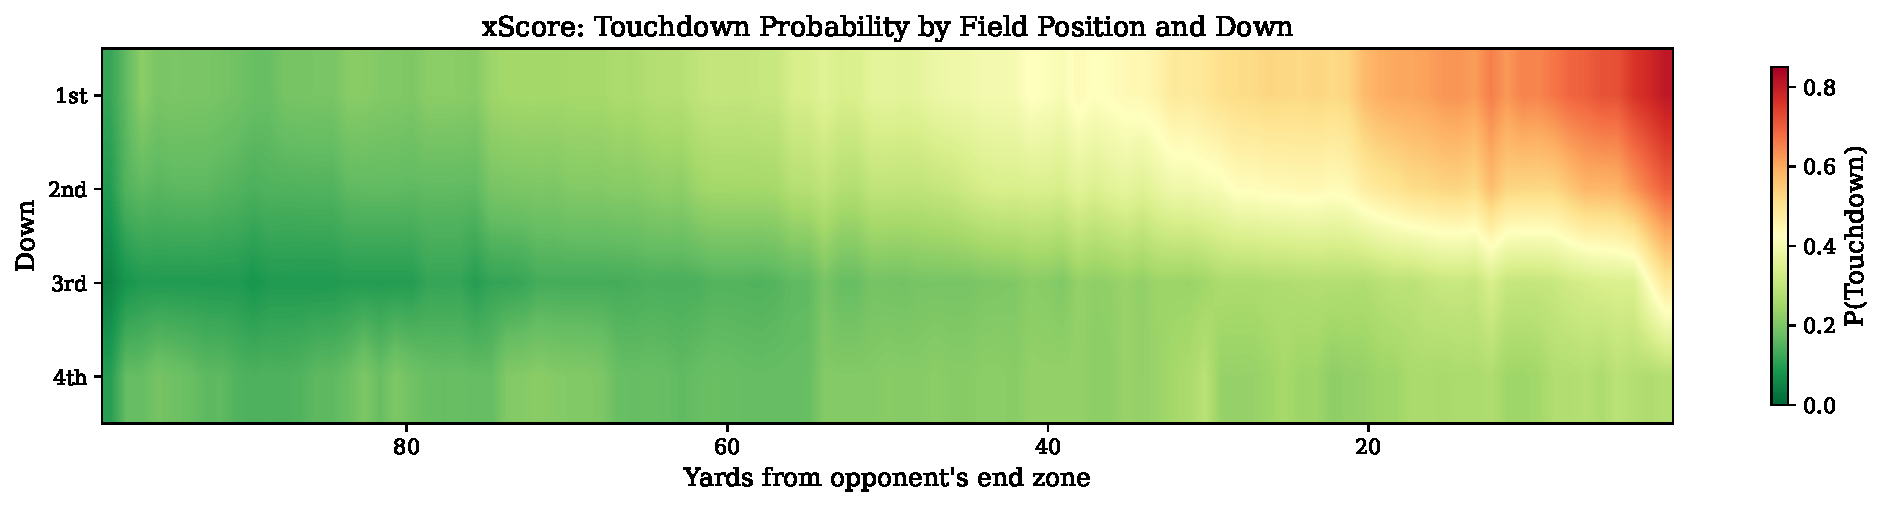
\includegraphics[width=\textwidth]{figures/fig2_field_heatmap.pdf}
  \caption{\xscore{} touchdown probability surface by field position and down
           (10 yards to go, neutral game state). The gradient reflects the
           model's learned relationship between proximity to the end zone and
           scoring probability, with diminishing returns as distance increases.}
  \label{fig:field-heatmap}
\end{figure}

\subsection{Interpretability via SHAP Values}
\label{sec:interpretability}

In addition to aggregate performance metrics and intuition validation,
the \xscore{} model is subjected to a SHAP (SHapley Additive exPlanations)
analysis \parencite{lundberg2017shap}. SHAP values decompose the prediction
for each individual observation into additive contributions from each feature,
grounded in cooperative game theory. Formally, for a prediction $\hat{p}_i$,
the SHAP value $\phi_j(i)$ for feature $j$ satisfies

\begin{equation}
  \hat{p}_i = \mathbb{E}[\hat{p}] + \sum_{j=1}^{K} \phi_j(i),
\end{equation}

where $\mathbb{E}[\hat{p}]$ is the unconditional mean prediction and $K$ is
the number of features \parencite{lundberg2017shap}. SHAP values for tree
ensembles are computed exactly in polynomial time via the TreeSHAP algorithm
\parencite{lundberg2017shap}, making them tractable for the full training
dataset.

Four interpretability checks are performed using SHAP analysis:

\begin{enumerate}
  \item \textbf{Field position dominance.} \texttt{yardline\_100} should rank
        as the single most important feature by mean absolute SHAP value,
        reflecting the well-established primacy of field position in
        touchdown probability. This is a necessary condition for the model to
        be considered domain-valid.

  \item \textbf{Down importance.} \texttt{down} should rank as the second
        most important feature, since later downs are associated with lower
        probability of drive continuation and eventual scoring.

  \item \textbf{Time effects.} \texttt{half\_seconds\_remaining} should
        contribute minimally for most game states -- time pressure only
        materially affects scoring probability in the final two minutes of
        each half -- and any systematic interaction with score differential
        should be consistent with known two-minute drill dynamics.

  \item \textbf{Red-zone indicator localization.} The \texttt{goal\_to\_go}
        and \texttt{red\_zone} binary features should exhibit localized SHAP
        effects concentrated inside the opponent's 20-yard line rather than
        diffuse contributions across all field positions, confirming that they
        capture the expected nonlinearity at the boundary between
        \texttt{yardline\_100} and the end zone.
\end{enumerate}

SHAP summary plots and feature importance rankings are reported in the
results chapter alongside the quantitative performance metrics, providing
a transparent audit trail of the model's learned decision structure.

\section{The Game Deserved Score Framework}
\label{sec:gds}

\subsection{Motivation: The Noisiness of Point Differential}

The most common summary statistic of NFL game performance is point differential:
the margin of victory or defeat at the final whistle. Point differential is
intuitively appealing and correlates with season outcomes at the aggregate
level \parencite{stern1991probability}, but it is a poor measure of within-game
performance quality. Scoring
events in American football are discrete and lumpy \parencite{lopez2018randomness}; a single play can produce
seven points while an extended drive producing sustained field position may
produce none. As a result, the final score frequently fails to reflect which
team controlled the game's probabilistic narrative.

Analysis of the 2018--2024 NFL seasons in the present study confirms this
systematically: approximately 25\% of regular-season games are won by the team
that gained fewer yards and converted fewer first downs than its opponent. Teams can -- and
frequently do -- lose the statistical battle while winning the scoreboard battle
through turnover returns, short fields, special teams scores, or simply higher
variance in the timing of their offensive execution. A team that accumulates
eight field-goal opportunities and converts three is not straightforwardly
inferior to a team that accumulates two touchdown opportunities and converts
both; yet point differential records only the nine-point and fourteen-point
outcomes and treats them identically regardless of the underlying process.

This motivates a framework that decomposes game-level performance into the
contributions of the underlying offensive, defensive, and special teams
processes, evaluated in a common unit that is directly comparable across games
and teams. The Game Deserved Score (\gds{}) framework serves this purpose.
\Cref{fig:pipeline} provides a schematic overview of the end-to-end
computation pipeline.

\begin{figure}[htbp]
  \centering
  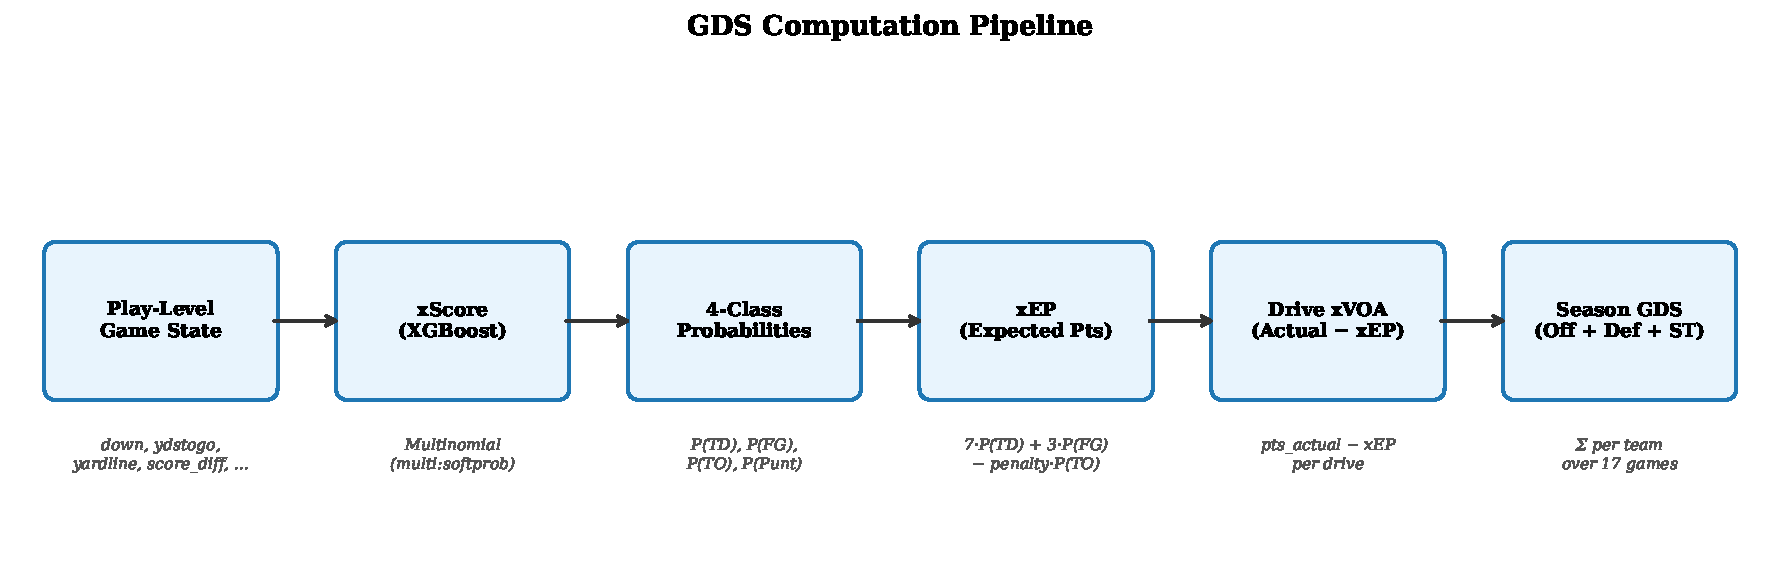
\includegraphics[width=\textwidth]{figures/fig9_pipeline_flowchart.pdf}
  \caption{End-to-end GDS computation pipeline. Situational game-state features
           feed into the multinomial \xscore{} model, producing four-class drive
           outcome probabilities that are converted to expected points (xEP).
           Drive-level value over average (xVOA) is aggregated to season-level
           GDS decomposed into offensive, defensive, and special-teams
           contributions.}
  \label{fig:pipeline}
\end{figure} The
central idea is analogous to the Expected Possession Value decomposition in
basketball analytics: rather than asking ``which team scored more?'', the
framework asks ``which team generated and suppressed scoring-probability at a
rate inconsistent with league expectations, and by how much?''
\parencite{cervone2016multiresolution}. The currency of this accounting is
the expected points value derived from the multinomial \xscore{} probability
vector introduced in \Cref{sec:xscore}: for each drive, the model's four-class
output is converted into a single expected-point figure representing what a
league-average team would score from the given situational state.

\subsection{Three-Component Decomposition}
\label{sec:gds-decomposition}

\gds{} decomposes game-level deserved performance into three additive channels:
offensive expected value over average (Off\_\xvoa{}), defensive expected value over average (Def\_\xvoa{}), and special teams value (ST\_Value).
The decomposition is exhaustive in the following sense: every drive in a game
is routed through exactly one of the three channels based on its scoring
outcome relative to the expected points at drive start.

\begin{itemize}
  \item \textbf{Offensive \xvoa{}} captures the degree to which the possession
        team's offensive execution generated points above or below the
        situational baseline. A team that consistently scored more points than
        expected from its drive-opening states accumulates positive offensive
        \xvoa{}.

  \item \textbf{Defensive \xvoa{}} captures the degree to which the defensive
        team suppressed the opponent's ability to generate points above
        expectation. It is derived directly from the opponent's offensive
        \xvoa{}, ensuring consistency of scale and eliminating the need for a
        separate defensive model.

  \item \textbf{Special Teams Value} (\textit{ST~Value}) captures the advantage
        or disadvantage conferred by the field position inherited at the start
        of each drive, relative to what that drive-start type typically yields
        across the league. It accounts for the value of returns, punting
        quality, kickoff coverage, and turnover field position in a unified
        framework.
\end{itemize}

The three channels partition every scoring-relevant action in the game. A
turnover that ends an offensive drive is penalized in offensive \xvoa{} (the
drive scores zero points against a positive expected-point baseline) and
rewarded in special teams value for the opponent (whose subsequent drive begins
at a superior starting position). A defensive stop that forces a three-and-out does not generate a
separate accounting entry; instead, it is reflected in the negative offensive
\xvoa{} of the opponent, which by the mirror formula (\Cref{sec:def-xvoa})
becomes a positive defensive \xvoa{} for the defending team. This structure
guarantees that no event is double-counted.

Formally, for a team $A$ in a game against opponent $B$, the Game Deserved
Score is defined as:

\begin{equation}
  \label{eq:gds}
  \gds(A) = \xvoa{}_{\mathrm{Off}}(A) + \xvoa{}_{\mathrm{Def}}(A)
             + \mathrm{ST}(A),
\end{equation}

where the three terms are defined and formalized in the subsections that
follow. All three terms are expressed in expected-point units: a
\gds{} of $+7.0$ means that the team generated the equivalent of one full
touchdown of net positive performance beyond what a league-average team
would have been expected to produce in identical circumstances.

\subsection{Offensive Value Added}
\label{sec:xvoa}

Offensive \xvoa{} measures the net difference between the points actually
scored on a drive and the expected points assigned to that drive's opening
state by the multinomial \xscore{} model (\Cref{sec:xscore}). The intuition
is straightforward: a drive that begins from a state where the model predicts
$\mathrm{xEP} = 2.1$ and ends in a touchdown (7 points) has generated $7 - 2.1
= 4.9$ points of value above expectation. A drive that begins from the same
state and ends in a punt (0 points) has generated $0 - 2.1 = -2.1$ points of
value relative to the baseline. The accumulated sum of these drive-level
differences across all of a team's possessions reflects the offensive
contribution that cannot be explained by the situational context alone.

This framing is analogous to the expected-goals framework in association
football analytics, where the accumulated difference between actual goals and
expected goals over a match captures shooting quality and finishing efficiency
beyond what shot location and context predict
\parencite{rathke2017expectedgoals}. In the present application, the outcome
space is expected points derived from the multinomial probability vector rather
than a single goal probability, and the accumulation occurs at the drive level
using actual points scored versus expected points at drive start.

\subsubsection{Drive-Level xVOA}

Under the multinomial model, offensive \xvoa{} is computed directly at the
drive level rather than through play-to-play deltas. Let $s_1^{(d)}$ denote
the situational state of the first play of drive $d$, and let
$\mathrm{xEP}(s_1^{(d)})$ be the expected points at that state as defined
in \Cref{eq:xep}. Let $\mathrm{pts}(d)$ denote the actual points scored on
drive $d$:

\begin{equation}
  \label{eq:pts-drive}
  \mathrm{pts}(d) =
    \begin{cases}
      7 & \text{if drive } d \text{ ends in an offensive touchdown}, \\
      3 & \text{if drive } d \text{ ends in a made field goal}, \\
      0 & \text{otherwise (punt, turnover, end of half, safety).}
    \end{cases}
\end{equation}

Safeties are classified under the zero-point category. Although a safety
yields two points for the \emph{defensive} team, the possession team's drive
scores zero; the opponent's two-point gain is captured through the subsequent
kickoff drive's starting field position, which enters the special teams
channel. Safeties occur on fewer than 0.5\% of drives, making their treatment
inconsequential to aggregate results.

The per-drive offensive value added is then the difference between actual
points and expected points:

\begin{equation}
  \label{eq:xvoa-drive}
  \xvoa{}^{(d)} = \mathrm{pts}(d) - \mathrm{xEP}\!\bigl(s_1^{(d)}\bigr).
\end{equation}

This formulation captures the full information content of the multinomial
model. A drive that begins in a state with $\mathrm{xEP} = 2.8$ (reflecting,
say, a 30\% TD probability, a 25\% FG probability, and moderate turnover risk)
and ends in a touchdown generates $\xvoa{}^{(d)} = 7 - 2.8 = +4.2$. The same
drive ending in a field goal generates $\xvoa{}^{(d)} = 3 - 2.8 = +0.2$ -- still
positive, reflecting that the team exceeded expectation, but capturing the
fact that a field goal from a favorable state represents only modest
overperformance. A drive ending in a punt generates $\xvoa{}^{(d)} = 0 - 2.8
= -2.8$, penalizing the failure to convert a state with substantial scoring
expectation. This graduated accounting -- distinguishing between a 7-point
outcome, a 3-point outcome, and a 0-point outcome -- is the primary advantage
of the multinomial approach over the binary model, which could only distinguish
between touchdown and not-touchdown.

\subsubsection{Game-Level Aggregation}

Offensive \xvoa{} for team $A$ in a game is the sum of per-drive values
across all of that team's drives in the game:

\begin{equation}
  \label{eq:xvoa-off}
  \xvoa{}_{\mathrm{Off}}(A) = \sum_{d \in \mathcal{D}(A)} \xvoa{}^{(d)}
    = \sum_{d \in \mathcal{D}(A)}
      \Bigl[\mathrm{pts}(d) - \mathrm{xEP}\!\bigl(s_{1}^{(d)}\bigr)\Bigr],
\end{equation}

where $\mathcal{D}(A)$ is the set of drives run by team $A$ in the game.
The interpretation is direct: offensive \xvoa{} is the aggregate difference
between actual points scored and the expected points that league-average
execution would have been expected to produce from the same sequence of
drive-opening states. A team that converts consistently above its situational
baseline accumulates positive offensive \xvoa{}; a team that fails to convert
from high-expected-point positions accumulates negative offensive \xvoa{}.

\subsection{Defensive Value Added}
\label{sec:def-xvoa}

A separate defensive probability model is not required in the \gds{} framework.
The defensive contribution of team $A$ in a game against team $B$ is defined
as the negative of the offensive \xvoa{} that team $B$ produced:

\begin{equation}
  \label{eq:xvoa-def}
  \xvoa{}_{\mathrm{Def}}(A) = -\,\xvoa{}_{\mathrm{Off}}(B).
\end{equation}

The logic is as follows. The offensive \xvoa{} of team $B$ measures the
aggregate points that team $B$'s offense generated beyond situational
expectation. Those points must have been generated against some defensive
unit -- and in a two-team game, that unit is team $A$'s defense. A high
offensive \xvoa{} for team $B$ therefore indicates that team $A$'s defense
was suppressed or beaten relative to what a league-average defense would have
allowed in the same situational sequence. Negating team $B$'s offensive \xvoa{}
converts this into a defensive penalty for team $A$. Symmetrically, if team $B$
generated negative offensive \xvoa{} (underperformed the situational baseline),
team $A$'s defense receives positive credit.

This mirror construction has two practical advantages. First, it guarantees
that the sum of offensive and defensive \xvoa{} contributions across both teams
in any single game is exactly zero: $\xvoa{}_{\mathrm{Off}}(A) +
\xvoa{}_{\mathrm{Def}}(B) + \xvoa{}_{\mathrm{Off}}(B) +
\xvoa{}_{\mathrm{Def}}(A) = 0$. The game-level \gds{} values for both teams
therefore differ only by the net effect of special teams play, which is not
in general zero-sum (both teams' special teams can add or subtract from
expected value independently). Second, the mirror construction avoids the
attribution ambiguity that would arise if defensive \xvoa{} were computed
directly from defensive plays (sacks, tackles for loss, pass deflections),
which overlap with the offensive drive sequence and would risk double-counting
plays that are already accounted for in the opponent's offensive \xvoa{}.

Positive defensive \xvoa{} means the defense held the opponent below its
expected offensive output. Negative defensive \xvoa{} means the defense
allowed the opponent to generate more points above expectation than the
league-average defense would have allowed against the same sequence of
situational states.

\subsection{Special Teams Value}
\label{sec:st-value}

Special teams play affects \gds{} through the starting field position it
confers at the beginning of each offensive drive. A kick returner who advances
a kickoff to the 35-yard line instead of the 25-yard line has, in effect,
transferred ten yards of field position to the subsequent possession -- which
the \xscore{} model will translate into higher starting expected points.
The Special Teams Value component quantifies this transfer.

\subsubsection{Drive Transition Types}
\label{sec:drive-transitions}

Each drive in the dataset is associated with a transition type that records
the event that initiated the possession. The raw \texttt{nflfastR} dataset
contains a richer set of transition labels, including rare variants such as
muffed punts, blocked kicks, and onside recoveries. These rare types are
consolidated into six canonical categories to ensure stable baseline
estimation:

\begin{table}[htbp]
  \centering
  \caption{Drive transition type taxonomy. Rare raw labels are consolidated
           into six canonical categories for stable baseline computation.}
  \label{tab:transitions}
  \small
  \begin{tabularx}{\textwidth}{l l X}
    \toprule
    \textbf{Canonical} & \textbf{Raw Subtypes} & \textbf{Description} \\
    \midrule
    \texttt{KICKOFF}
      & Kickoff, onside kick, muffed kickoff
      & Possession via any kickoff variant \\[3pt]
    \texttt{PUNT}
      & Punt, blocked punt, muffed punt
      & Possession via punt or blocked/muffed punt \\[3pt]
    \texttt{MISSED\_FG}
      & Missed FG, blocked FG, muffed FG
      & Possession via missed or blocked FG attempt \\[3pt]
    \texttt{INTERCEPTION}
      & Interception
      & Possession via forward pass interception \\[3pt]
    \texttt{FUMBLE}
      & Fumble
      & Possession via defensive fumble recovery \\[3pt]
    \texttt{DOWNS}
      & Downs
      & Possession via failed 4th-down conversion \\
    \bottomrule
  \end{tabularx}
\end{table}

The motivation for this consolidation is statistical stability. Rare events
such as blocked field goals occur fewer than thirty times per season across
the entire league; computing a reliable mean starting $\mathrm{xEP}$ from such
sparse samples requires either pooling with a parent category or accepting
high-variance estimates. The consolidation in \Cref{tab:transitions} groups
each rare type into the parent category that best matches its typical
starting field position, and the resulting canonical categories each contain
hundreds of drives in the training window.

\subsubsection{Baseline Computation}

The expected starting $\mathrm{xEP}$ for each canonical transition type is
estimated empirically from the training data (seasons 2018--2024) as the
arithmetic mean of the $\mathrm{xEP}$ value at the first play of all drives of
that type:

\begin{equation}
  \label{eq:st-baseline}
  \mu_{\tau} = \frac{1}{|\mathcal{D}_{\tau}|}
    \sum_{d \in \mathcal{D}_{\tau}} \mathrm{xEP}\!\bigl(s_1^{(d)}\bigr),
\end{equation}

where $\mathcal{D}_{\tau}$ is the set of all training-window drives that begin
with transition type $\tau$ drawn from the six canonical categories defined in
\Cref{tab:transitions}, and $s_1^{(d)}$ is the first play of drive $d$.

Several design choices in this formula warrant comment. First, the baseline
uses \emph{actual} $\mathrm{xEP}$ values at the observed first play rather than
a synthetic neutral state (e.g., a fixed yardline and down). This means that
the baseline implicitly captures the real game context in which each
transition type tends to occur: kickoffs, for instance, often occur
early in drives following scoring plays, when the clock situation and score
differential create a particular probabilistic context. The baseline is
therefore an empirical distribution over real game states, not a
stylized average.

Second, the baseline is computed once on the training window and held fixed
for all subsequent applications -- including the 2025 test set and any
out-of-distribution evaluation. This prevents leakage: the expected value
for a transition type on a given test play is derived only from training-window
data.

Third, individual drive first-play $\mathrm{xEP}$ values reflect the full
situational state (field position, down, distance, score differential, time),
so the baseline $\mu_\tau$ implicitly integrates over the typical game states
that accompany each transition type. A team that consistently receives good
kickoff returns will systematically start kickoff drives at a higher
$\mathrm{xEP}$ than $\mu_{\texttt{KICKOFF}}$, and this difference is credited
to special teams value.

\subsubsection{Per-Drive Special Teams Value}

For each drive $d$ with transition type $\tau(d)$, the per-drive special
teams value is the deviation of the actual starting $\mathrm{xEP}$ from the
type-specific baseline:

\begin{equation}
  \label{eq:st-drive}
  \mathrm{ST}^{(d)} = \mathrm{xEP}\!\bigl(s_1^{(d)}\bigr) - \mu_{\tau(d)}.
\end{equation}

A positive per-drive ST~value means the drive began from a more favorable
field position than the league average for that transition type. A negative
value means the drive began from a less favorable position.

\subsubsection{Game-Level Aggregation}

The game-level special teams value for team $A$ is the sum of per-drive
ST values across all drives in the game:

\begin{equation}
  \label{eq:st-game}
  \mathrm{ST}(A) = \sum_{d \in \mathcal{D}(A)} \mathrm{ST}^{(d)}.
\end{equation}

This formulation rewards teams that consistently secure superior starting
positions across all their drives -- regardless of whether those superior
positions were obtained via kick returns, punt coverage, or the opponent's
failed fourth-down attempts.

\subsection{Attribution Rules and Turnover Handling}
\label{sec:attribution}

A potential concern with any decomposition framework is double-counting:
could the same underlying play contribute to multiple components? The
structure of the \gds{} framework is designed to prevent this, and the
treatment of turnovers provides the clearest illustration.

When the offense commits a turnover -- an interception or fumble recovery by
the defense -- the following accounting occurs:

\begin{enumerate}
  \item \textbf{Offensive \xvoa{} of the turning team.} The drive containing
        the turnover terminates at $\mathrm{pts}(d) = 0$. The drive-level
        \xvoa{} is $0 - \mathrm{xEP}(s_1^{(d)})$, which is negative whenever
        the drive began from a state with positive expected points (as
        virtually all drives do). The full cost of the failed drive is
        absorbed by the turning team's offensive \xvoa{}.

  \item \textbf{Special teams value of the receiving team.} The opponent's
        subsequent drive begins with a transition type of
        \texttt{INTERCEPTION} or \texttt{FUMBLE}, and its starting
        $\mathrm{xEP}$ is compared to the $\mu_{\texttt{INTERCEPTION}}$ or
        $\mu_{\texttt{FUMBLE}}$ baseline. Turnovers often occur near midfield
        or in opposition territory, so the receiving team frequently begins
        from a higher-than-average starting position for that transition type,
        generating positive special teams value. However, this credit goes only
        to the starting field position advantage -- not to the act of forcing
        the turnover itself.

  \item \textbf{Defensive \xvoa{} of the receiving team.} The receiving team's
        defensive \xvoa{} is the negative of the turning team's offensive
        \xvoa{} -- which, as established in point~1, already accounts for the
        failed drive including the turnover. No additional defensive entry is
        created for the turnover play.
\end{enumerate}

The result is a clean partition: the cost of the turnover is borne entirely
by the turning team's offensive channel; the positional benefit of the
resulting field position is credited to the receiving team's special teams
channel; and the defensive channel receives credit for the overall
suppression of the opponent's offensive \xvoa{} without any separate
entry for the turnover event. No play is counted in more than one channel.

\subsection{Formal Properties of \gds{}}
\label{sec:gds-properties}

The \gds{} framework satisfies several formal properties that support its
use as an analytical tool.

\paragraph{Zero-sum decomposition.}
For any single game between teams $A$ and $B$:
\begin{equation}
  \label{eq:zero-sum}
  \bigl[\xvoa{}_{\mathrm{Off}}(A) + \xvoa{}_{\mathrm{Def}}(A)\bigr]
  +
  \bigl[\xvoa{}_{\mathrm{Off}}(B) + \xvoa{}_{\mathrm{Def}}(B)\bigr]
  = 0.
\end{equation}
This follows directly from the mirror definition in \Cref{eq:xvoa-def}:
\begin{align*}
  \xvoa{}_{\mathrm{Def}}(A) &= -\xvoa{}_{\mathrm{Off}}(B), \\
  \xvoa{}_{\mathrm{Def}}(B) &= -\xvoa{}_{\mathrm{Off}}(A),
\end{align*}
so the four terms cancel pairwise. Special teams values are \emph{not} constrained to sum to
zero across the two teams, because the baselines $\mu_\tau$ are estimated
from the full league distribution rather than from within-game comparisons.
Both teams can receive positive special teams value in the same game if both
enjoyed above-average starting positions for their respective transition types.
The total \gds{} across both teams in a game is therefore equal to the sum of
their special teams values:

\begin{equation}
  \gds(A) + \gds(B) = \mathrm{ST}(A) + \mathrm{ST}(B).
\end{equation}

\paragraph{Unified scale.}
All three components of \gds{} and \gds{} itself are expressed in
expected-point units. This means that contributions from different phases of
the game -- a dominant passing performance, a turnover-inducing defensive
scheme, and a 60-yard kickoff return -- are directly comparable on the same
numerical scale. A special teams value of $+1.0$ represents the same
point-value advantage as an offensive \xvoa{} of $+1.0$: one additional
expected point of net positive performance relative to a league-average
baseline.

\paragraph{Additivity across games.}
Because each game's \gds{} is computed in the same units on the same
underlying \xscore{} model, game-level \gds{} values are additive across
multiple games. Season-level \gds{} totals are simply the sum of weekly
values, and the season decomposition into offensive, defensive, and special
teams channels is preserved. This permits season-long comparisons of component
contributions and enables the archetype analyses presented in
\Cref{sec:archetype-analysis}.

\paragraph{Decomposability.}
The additive structure \gds{} = offensive + defensive + special teams is
preserved at every aggregation level: per game, per week, per season, or
across selected subsets of games (e.g., playoff games only). This
decomposability allows analysts to isolate the contribution of any single
channel to a team's overall \gds{} trajectory, which is the analytical
foundation of the archetype classification in \Cref{sec:archetype-analysis}.

\section{Archetype Analysis: Statistical Design}
\label{sec:archetype-analysis}

The preceding sections establish the \xscore{} model (\Cref{sec:xscore}) and
the \gds{} framework (\Cref{sec:gds}) as tools for measuring team performance
in expected-point units, decomposed into offensive, defensive, and
special teams channels. This section describes how those measurements are used
to test a canonical claim in American football discourse: that defensive
strength is a more reliable pathway to postseason success than offensive
strength. The section proceeds from the operationalization of the research
question through to the sample size and power considerations that govern the
interpretation of results.

% ============================================================
\subsection{Research Question and Hypotheses}
\label{sec:hypotheses}
% ============================================================

The popular aphorism ``defense wins championships'' -- sometimes rendered in
its fuller form as ``offense wins games, defense wins championships'' -- is
an empirical claim about the relative importance of defensive performance
in determining postseason outcomes \parencite{robst2011defense}.
\textcite{robst2011defense} examined this claim using conventional metrics
and found mixed support at best; the present analysis revisits the question
with the higher-resolution decomposition afforded by \gds{}-derived \xvoa{}
values.

To give the claim precise, falsifiable content, it is decomposed into three
testable hypotheses. Each hypothesis is stated in terms of the archetype
variables defined in \Cref{sec:ivs}.

\begin{description}
  \item[H1 (Postseason advancement).] Defense-dominant team-seasons, defined
        by a negative offense share (i.e., teams for which defensive
        \xvoa{} contributes more to overall \gds{} than offensive \xvoa{}),
        achieve higher mean playoff-win totals than offense-dominant
        team-seasons among playoff qualifiers.

  \item[H2 (Super Bowl over-representation).] Super Bowl winners are
        disproportionately drawn from defense-dominant team-seasons relative to
        the base rate of defense dominance among all playoff qualifiers.

  \item[H3 (Correlation asymmetry).] Defensive \xvoa{} per game exhibits a
        stronger monotonic association with playoff wins among playoff teams than
        offensive \xvoa{} per game does.
\end{description}

If all three hypotheses are supported, the evidence is consistent with the
``defense wins championships'' narrative. Rejection of any single hypothesis
constitutes evidence against the claim and shifts the interpretive burden toward
alternative explanations -- including the possibility that offensive quality is
equally or more important, or that the claim only holds in specific eras or
roster-strength contexts. The analysis is designed so that the three hypotheses
are logically independent: a team-season structure that would support H1 (e.g.,
defense-dominant teams advancing further) need not automatically support H2
(which concerns the extreme tail of one Super Bowl winner per season) or H3
(which concerns marginal correlations across the full playoff sample). This
independence ensures that any finding is not an artifact of a single operationalization.

% ============================================================
\subsection{Independent Variables}
\label{sec:ivs}
% ============================================================

The analysis uses four independent variables derived from \gds{}-level
aggregates at the team-season level. Per-game averages are used throughout
to adjust for the small number of team-seasons that played more or fewer
games due to schedule irregularities. \Cref{tab:ivs} summarizes the variables,
their definitions, and their intended interpretations.

\begin{table}[htbp]
  \centering
  \caption{Independent variables in the archetype analysis. All variables are
           computed at the team-season level using regular-season games only.
           Per-game averages remove the effect of schedule length variation.}
  \label{tab:ivs}
  \begin{tabularx}{\textwidth}{llX}
    \toprule
    \textbf{Variable} & \textbf{Type} & \textbf{Definition} \\
    \midrule
    \texttt{offense\_share}
      & Continuous $[-1, +1]$
      & Proportion of total absolute \xvoa{} attributable to the offense
        (see \Cref{eq:offense-share}). Positive values indicate
        offense-dominant teams; negative values indicate defense-dominant teams. \\[6pt]
    \texttt{gds\_per\_game}
      & Continuous
      & Mean \gds{} per regular-season game. Measures overall team quality
        in expected-point units, independent of the offensive/defensive
        split. \\[6pt]
    \texttt{off\_xvoa\_per\_game}
      & Continuous
      & Mean offensive \xvoa{} per regular-season game. Direct measure of
        offensive output above or below situational expectation. \\[6pt]
    \texttt{def\_xvoa\_per\_game}
      & Continuous
      & Mean defensive \xvoa{} per regular-season game. Direct measure of
        defensive suppression above or below situational expectation.
        Positive values indicate above-average defensive performance. \\
    \bottomrule
  \end{tabularx}
\end{table}

The key analytical variable is \texttt{offense\_share}, which isolates the
\emph{balance} between offensive and defensive contribution independently of
overall team quality. It is defined as:

\begin{equation}
  \label{eq:offense-share}
  \texttt{offense\_share} =
  \frac{\texttt{off\_xvoa\_per\_game}}
       {|\texttt{off\_xvoa\_per\_game}| + |\texttt{def\_xvoa\_per\_game}| + \varepsilon},
\end{equation}

where $\varepsilon = 0.01$ is a small regularization constant that prevents
division by zero for teams with negligible \xvoa{} in both channels. The
denominator is the sum of the absolute magnitudes of the two \xvoa{} components,
so the ratio measures the fraction of the team's total absolute performance
attributable to offense. The $\varepsilon$ term does not materially affect the
result for any team with non-trivial \xvoa{} values, since realistic per-game
\xvoa{} magnitudes are on the order of $1$--$12$ expected-point units per game.

The resulting variable ranges from $-1$ to $+1$ by construction. A value of
$+1$ would correspond to a team whose entire positive performance derives from
offense with zero defensive contribution; a value of $-1$ would correspond to
the symmetric defensive extreme. In practice, most team-seasons fall in the
range $[-0.6, +0.6]$, reflecting the empirical reality that competitive NFL
teams generate meaningful contributions from both phases. The threshold values
used in the Cohen's d analysis (\Cref{sec:cohens-d}) are $+0.3$ for
offense-dominant and $-0.3$ for defense-dominant, chosen to separate teams
with a clear lean from those near the boundary.

The variables \texttt{off\_xvoa\_per\_game} and \texttt{def\_xvoa\_per\_game}
are included as component-level predictors in the logistic regression and OLS
models described in \Cref{sec:stat-tests}. Using components rather than
\texttt{offense\_share} alone allows the models to estimate whether it is the
absolute level of defensive performance -- rather than merely its dominance
relative to offense -- that predicts Super Bowl success and playoff advancement.
The \texttt{gds\_per\_game} variable serves as a quality control variable in
the OLS model, ensuring that any offense-share effect on playoff wins is not
simply a proxy for overall team strength.

As a robustness check for schedule-strength confounding, the OLS regression
is re-estimated with an opponent-quality control variable
(\texttt{opp\_avg\_gds}). This variable is constructed via a leave-one-out
procedure: for each team-season $i$, the mean \gds{}/game of all opponents
faced during the regular season is computed, excluding the focal team's own
contribution to those opponents' schedules. The leave-one-out construction
prevents the mechanical correlation that would arise if a team's own quality
inflated its opponents' apparent strength (since each opponent's \gds{}
partially reflects having played the focal team). If the offensive advantage
documented in the primary analysis is an artifact of schedule imbalance -- for
example, if offense-dominant teams systematically face weaker schedules -- then
including \texttt{opp\_avg\_gds} as a covariate should attenuate or eliminate
the offensive \xvoa{} coefficient in the controlled regression.

% ============================================================
\subsection{Dependent Variables}
\label{sec:dvs}
% ============================================================

The analysis uses three dependent variables that capture postseason outcomes
at increasing levels of selectivity. \Cref{tab:dvs} summarizes the variables
and their measurement properties.

\begin{table}[htbp]
  \centering
  \caption{Dependent variables in the archetype analysis. Playoff wins counts
           actual games played and won in the postseason; a bye week is not
           treated as a win because no game was played.}
  \label{tab:dvs}
  \begin{tabularx}{\textwidth}{llX}
    \toprule
    \textbf{Variable} & \textbf{Type} & \textbf{Description} \\
    \midrule
    \texttt{win\_pct}
      & Continuous $[0, 1]$
      & Regular-season win fraction. Used to assess whether offensive and
        defensive \xvoa{} components predict season-level success. \\[6pt]
    \texttt{playoff\_wins}
      & Ordinal integer $\{0, 1, 2, 3, 4\}$
      & Number of postseason games won. A value of $0$ indicates either
        missing the playoffs or a first-round exit. A Super Bowl winner
        receives 3 if they had a first-round bye (top seeds in all
        seasons) or 4 if they played the Wild Card round. \\[6pt]
    \texttt{won\_super\_bowl}
      & Binary $\{0, 1\}$
      & Indicator for whether the team won the Super Bowl in that
        season. \\
    \bottomrule
  \end{tabularx}
\end{table}

The decision to measure playoff success as \texttt{playoff\_wins} rather than
a binary playoff-appearance indicator reflects the hierarchical structure of
the NFL postseason. Making the playoffs requires above-average regular-season
performance, but it is a threshold event: a 12-win team that loses in the
Wild Card round and an 8-win team that receives a first-round bye and also
loses in the Divisional round are both credited with zero playoff wins. The
ordinal measure distinguishes these outcomes and captures the degree of
postseason advancement, which is the more theoretically relevant quantity for
testing whether team archetypes predict deep runs.

It is important to note that bye weeks are not counted as wins.
During the 2018--2019 seasons, the NFL's six-team playoff bracket granted two
first-round byes per conference. From 2020 onward, the expanded seven-team
bracket reduced this to one bye per conference. Across the study
window, a team with a first-round bye that won three subsequent games is
credited with three playoff wins, not four. This design ensures that
\texttt{playoff\_wins} reflects actual game performance rather than seeding
advantages, which is consistent with the framework's general philosophy of
measuring performance against outcomes rather than structural position.

% ============================================================
\subsection{Statistical Tests}
\label{sec:stat-tests}
% ============================================================

Five statistical procedures are employed, each motivated by the measurement
level and distributional properties of the variables involved.

\subsubsection{Spearman Rank Correlation}
\label{sec:spearman}

The primary test of H1 and H3 uses the Spearman rank correlation coefficient
between \texttt{offense\_share} and \texttt{playoff\_wins}, computed on the
subsample of playoff team-seasons. The Spearman coefficient is appropriate here
for two reasons. First, \texttt{playoff\_wins} is an ordinal variable with a
bounded range of 0--4; treating it as interval-scaled for Pearson correlation
would impose an equal-spacing assumption that may not hold
(the difficulty of advancing from Round 2 to Round 3 is not necessarily
identical to that of advancing from Round 1 to Round 2). Second, the
monotonic but potentially non-linear nature of the relationship between team
balance and playoff success is better captured by a rank-based measure that
does not impose linearity.

For H3, the Spearman correlation is computed separately for offensive
\xvoa{}/game versus playoff wins and defensive \xvoa{}/game versus playoff
wins. The magnitudes of the two coefficients are then compared to determine
which component exhibits the stronger association with playoff advancement.

\subsubsection{Pearson Correlation}

Pearson product-moment correlations are computed between offensive
\xvoa{}/game and win percentage, and between defensive \xvoa{}/game and win
percentage, using all 224 team-seasons. The use of Pearson rather than
Spearman is appropriate here because win percentage is a continuous
proportion that is approximately normally distributed at the team-season
level, and the linear relationship between per-game \xvoa{} and season win
rate is theoretically motivated by the additive structure of the \gds{}
framework.

These correlations serve as a consistency check: if the \gds{} decomposition
is well-calibrated, both offensive and defensive \xvoa{} should exhibit strong
positive correlations with win rate, confirming that the components measure
genuine performance signal. The relative magnitudes of the two correlations
provide initial evidence bearing on H3.

\subsubsection{Binary Logistic Regression}
\label{sec:logistic}

To test H2, a binary logistic regression model is estimated with
Super Bowl victory as the outcome variable and offensive and defensive
\xvoa{}/game as predictors across all 224 team-seasons:

\begin{equation}
  \label{eq:logistic}
  \log \frac{P(\texttt{won\_SB} = 1)}{P(\texttt{won\_SB} = 0)}
  = \beta_0
    + \beta_1 \cdot \texttt{off\_xvoa/g}
    + \beta_2 \cdot \texttt{def\_xvoa/g}.
\end{equation}

The coefficients $\beta_1$ and $\beta_2$ measure the change in log-odds of
Super Bowl victory associated with a one-unit increase in offensive or
defensive \xvoa{} per game, holding the other component constant. A finding
of $|\hat{\beta}_2| > |\hat{\beta}_1|$ would be consistent with H2 in the
sense that defensive \xvoa{} has greater marginal predictive value for the
championship outcome. The model follows the standard formulation of binary
logistic regression as described in \textcite{hosmer2013logistic}.

Standard errors, Wald $z$-statistics, and $p$-values are reported for each
coefficient. Confidence intervals are constructed at the 95\% level. The
model is estimated by maximum likelihood; convergence is assessed by
inspecting the log-likelihood at each iteration.

\subsubsection{Ordinary Least Squares Regression}

An OLS regression of \texttt{playoff\_wins} on \texttt{offense\_share} and
\texttt{gds\_per\_game} is estimated across all 224 team-seasons:

\begin{equation}
  \label{eq:ols}
  \texttt{playoff\_wins}_i
  = \alpha
    + \gamma_1 \cdot \texttt{offense\_share}_i
    + \gamma_2 \cdot \texttt{gds\_per\_game}_i
    + \varepsilon_i.
\end{equation}

The inclusion of \texttt{gds\_per\_game} as a covariate is critical: without
it, any observed association between \texttt{offense\_share} and
\texttt{playoff\_wins} could be confounded by overall team quality. Strong
teams advance further in the playoffs regardless of their offensive/defensive
balance; the coefficient on \texttt{offense\_share} is interpretable only after
this quality effect is partialled out. The coefficient $\hat{\gamma}_1$
therefore measures the marginal effect of shifting the balance between offensive
and defensive \xvoa{} on expected playoff wins, holding overall \gds{} per game
constant.

Although \texttt{playoff\_wins} is technically ordinal rather than continuous,
OLS on ordinal outcomes with a small number of categories is widely used in
applied social-science research and provides interpretable coefficient estimates
\parencite{long1997regression}. Because the outcome is zero-inflated
(approximately 58\% of team-seasons have zero playoff wins), residuals are
heteroscedastic; all reported standard errors and $p$-values use
heteroscedasticity-consistent (HC3) estimates. The Spearman correlations
(\Cref{sec:spearman}) serve as a robustness check that does not impose
linearity or equal-interval assumptions.

\subsubsection{Cohen's \textit{d} Effect Size}
\label{sec:cohens-d}

To quantify the practical magnitude of any difference in playoff advancement
between offense-dominant and defense-dominant teams, Cohen's $d$ is computed
as the standardized mean difference:

\begin{equation}
  \label{eq:cohens-d}
  d = \frac{\bar{x}_{\mathrm{off}} - \bar{x}_{\mathrm{def}}}{s_p},
  \qquad
  s_p = \sqrt{\frac{(n_{\mathrm{def}} - 1)\,s_{\mathrm{def}}^2
                    + (n_{\mathrm{off}} - 1)\,s_{\mathrm{off}}^2}
                   {n_{\mathrm{def}} + n_{\mathrm{off}} - 2}},
\end{equation}

where $\bar{x}_{\mathrm{def}}$ and $\bar{x}_{\mathrm{off}}$ are the mean
\texttt{playoff\_wins} for defense-dominant
($\texttt{offense\_share} < -0.3$) and offense-dominant
($\texttt{offense\_share} > +0.3$) team-seasons across all 224 observations, and
$s_p$ is the pooled standard deviation \parencite{cohen1988statisticalpower}.
Non-playoff team-seasons receive \texttt{playoff\_wins} $= 0$, so the effect
size captures both the selection effect (making the playoffs) and the
advancement effect (winning once there).

The conventional thresholds proposed by \textcite{cohen1988statisticalpower}
are used for interpretation: $|d| < 0.2$ is negligible, $|d| \approx 0.2$
is small, $|d| \approx 0.5$ is medium, and $|d| \approx 0.8$ or larger is
large. A positive $d$ indicates that offense-dominant teams win more playoff
games on average; a negative $d$ would indicate defense-dominant teams
perform better. The effect size
is reported alongside the raw means and standard deviations to support
substantive interpretation independent of statistical significance.

% ============================================================
\subsection{Quartile Analysis}
\label{sec:quartile-analysis}
% ============================================================

As a non-parametric complement to the regression analyses, team-seasons are
partitioned into four equal-sized groups (quartiles) by \texttt{offense\_share}.
Quartile one (Q1) contains the most defense-dominant team-seasons; quartile
four (Q4) contains the most offense-dominant team-seasons. For each quartile,
the analysis reports the playoff appearance rate, the mean \texttt{playoff\_wins}
conditional on playoff qualification, and the Super Bowl win count.

The quartile design is preferred over binary splits for two reasons. First, it
is non-parametric: it does not assume a particular functional form for the
relationship between \texttt{offense\_share} and postseason outcomes, and it
does not require the analyst to specify a threshold separating
``offense-dominant'' from ``defense-dominant'' before seeing the data. Second,
equal-sized groups ensure that each quartile contributes equally to the
descriptive picture, rather than allowing an extreme but sparsely populated
tail to dominate the comparison. If the ``defense wins championships'' narrative
is supported, the playoff appearance rate and mean playoff wins should increase
monotonically from Q4 (most offense-dominant) to Q1 (most defense-dominant).

% ============================================================
\subsection{Era Comparison}
\label{sec:era-comparison}
% ============================================================

The study window spans two distinct regulatory eras. The 2018--2019 period
comprises two seasons under the six-team postseason bracket, in which two
first-round byes per conference were awarded to the top two seeds. The
expanded seven-team bracket was adopted from the 2020 season onward, granting
only the top seed per conference a bye. For the era comparison, the sample is
split at the 2020--2021 boundary (2018--2020 vs.\ 2021--2024) to create
sub-samples of roughly comparable size, noting that the 2020 season already
operated under the expanded bracket. The bracket expansion increases the
number of playoff games played per conference by one and modestly lowers the
average seeding quality of the playoff field.

Beyond the structural bracket change, the 2021--2024 era has seen an increase
in rule enforcement protecting quarterbacks and receivers, which some
commentators argue has favored offensive production \parencite{barnwell2019passingrevolution,nflscoring2023trends}. Whether this translates
into a weakening of the ``defense wins championships'' association is an
empirically testable directional question.

For each era, the Spearman rank correlation between \texttt{offense\_share} and
\texttt{playoff\_wins} is computed on the respective playoff subsample and
compared in direction and magnitude. This comparison is explicitly flagged as
directional and exploratory. The per-era playoff subsamples contain
approximately 36 team-seasons (2018--2020) and approximately 58 team-seasons
(2021--2024), sample sizes that are insufficient for formal significance tests
of the difference between two Spearman coefficients. The era comparison is
therefore interpreted as a descriptive pattern and a motivation for future
work with longer time horizons, not as a definitive finding about trend.

% ============================================================
\subsection{Quadrant Analysis}
\label{sec:quadrant-analysis}
% ============================================================

The regression and quartile analyses treat offensive and defensive strength as
exchangeable inputs to the same scalar \texttt{offense\_share} index. A
complementary analysis separates the two dimensions explicitly by constructing
a $2 \times 2$ quadrant matrix. This approach is restricted to the top 25\%
of team-seasons by \texttt{gds\_per\_game} -- those with demonstrably elite
overall quality -- to remove the confound that poor performance in both phases
simultaneously drives down the entire distribution.

Within this elite subsample, teams are median-split on offensive and defensive
\xvoa{}/game separately, creating four quadrants:

\begin{table}[htbp]
  \centering
  \caption[Quadrant classification for elite team-seasons]{Quadrant classification for elite team-seasons (top-quartile
           \gds{} per game). The median split is applied separately within
           the elite subsample for offensive and defensive \xvoa{} per game.
           Each cell reports the number of team-seasons, playoff appearance
           rate, and mean playoff wins.}
  \label{tab:quadrants}
  \begin{adjustbox}{max width=\textwidth}
  \begin{tabular}{lcc}
    \toprule
    & \textbf{Above-median defense} & \textbf{Below-median defense} \\
    \midrule
    \textbf{Above-median offense}
      & \textit{Elite Both} (Q-BO)
      & \textit{Offense Only} (Q-OO) \\[4pt]
    \textbf{Below-median offense}
      & \textit{Defense Only} (Q-DO)
      & \textit{Neither} (Q-NN) \\
    \bottomrule
  \end{tabular}
  \end{adjustbox}
\end{table}

The \textit{Elite Both} quadrant (Q-BO) contains elite team-seasons with
above-median performance in both phases; \textit{Offense Only} (Q-OO) contains
those with strong offense but weaker defense; \textit{Defense Only} (Q-DO)
contains those with strong defense but weaker offense; and \textit{Neither}
(Q-NN) contains elite teams whose quality derives more from special teams and
scheduling than from either major phase.

The quadrant analysis tests a more nuanced version of the championship claim.
If the ``defense wins championships'' narrative is correct in its strong form,
Q-DO should generate more Super Bowl winners than Q-OO among elite team-seasons.
If the narrative is incorrect and offensive excellence dominates, Q-OO should
generate more. If both phases are equally important at the elite level, the
champion rate should be similar across Q-BO, Q-OO, and Q-DO, with Q-NN
contributing the fewest. The population of 56 elite team-seasons (top-quartile
out of 224) is small enough that stochastic variation will be substantial;
results are therefore interpreted descriptively alongside the full-sample
statistical tests.

% ============================================================
\subsection{Sample Size and Statistical Power}
\label{sec:sample-size}
% ============================================================

The analysis is conducted on a sample of 224 team-seasons (32 teams across
7 seasons, 2018--2024). The playoff subsample comprises approximately 94
team-seasons (roughly 13--14 per season, accounting for bye-team inclusion
and the bracket expansion in 2020). The Super Bowl winner subsample contains
exactly 7 observations, one per season.

These sample sizes have different implications for the statistical power of each
procedure. The Pearson and Spearman correlations involving all 224 team-seasons
or the 94-season playoff subsample are reasonably powered to detect medium to
large effect sizes. Using the approximation for Pearson correlation power
\parencite{cohen1988statisticalpower}, a sample of $n = 94$ provides
approximately 80\% power to detect a true population correlation of
$|\rho| \approx 0.29$ at $\alpha = 0.05$ (two-tailed). For $n = 224$ the
corresponding detectable correlation drops to $|\rho| \approx 0.19$.
Effect sizes below these thresholds may exist but will be statistically
undetectable in the present data.

The binary logistic regression (\Cref{sec:logistic}) is the most power-limited
procedure. With 7 Super Bowl winners and approximately 87 non-winners in the
playoff subsample, the effective event rate is approximately 7\%. Standard
guidelines for logistic regression suggest a minimum of 10--15 events per
predictor variable \parencite{hosmer2013logistic}; the present model uses 2
predictors, implying a minimum of 20 events for reliable coefficient estimation.
The observed 7 events fall well below this threshold. The logistic regression
results are therefore interpreted as directional and exploratory. Coefficient
magnitudes and signs are reported, but $p$-values and confidence intervals are
treated as approximate given the small event count, and the model is used
primarily to examine whether defensive \xvoa{} has higher discriminative
association with the championship outcome than offensive \xvoa{}.

The Cohen's $d$ comparison between offense-dominant and defense-dominant
playoff teams depends on the number of team-seasons satisfying the threshold
criteria ($|\texttt{offense\_share}| > 0.3$). The approximately equal split
of the playoff sample across the offense-share spectrum yields group sizes in
the range of 20--30 per extreme, sufficient to detect a medium effect
($d \approx 0.5$) with approximately 60--70\% power at $\alpha = 0.05$.
This is below the conventional 80\% threshold, which means that a true medium
effect may go undetected. All effect sizes are therefore reported regardless
of statistical significance, with the understanding that the present study is
better characterized as exploratory-confirmatory in nature than as a
definitive hypothesis test.

The era comparison (\Cref{sec:era-comparison}) involves the smallest per-era
subsamples (approximately 36 and 58 playoff team-seasons) and is explicitly
treated as exploratory throughout. No formal inference about era differences
is drawn from these subsamples; the comparison is presented to orient future
work with longer data windows.

Across all analyses, statistical significance is assessed at $\alpha = 0.05$.
Spearman and Pearson $p$-values are reported two-tailed. The five
statistical procedures test different operationalizations of the same
directional hypothesis rather than strictly independent hypotheses: they are
designed to converge or diverge as a coherent body of evidence, not to control a
family-wise error rate across independent discoveries. The inferential
conclusion rests on the consistency and direction of results across all
procedures, not on any single $p$-value crossing a threshold. Nevertheless, as
a robustness check, Holm--Bonferroni-adjusted $p$-values are reported alongside
unadjusted values in the results (\Cref{sec:archetype-findings}). Under this
correction, all five primary tests remain significant at $\alpha = 0.05$,
confirming that the conclusions are not an artifact of multiple testing.



% Chapter 4: Results
\chapter{Results}
\label{ch:results}

This chapter presents the empirical findings. \Cref{sec:model-performance} reports \xscore{} model accuracy and calibration. \Cref{sec:gds-validation} validates the Game Deserved Score framework against actual game outcomes. \Cref{sec:archetype-findings} presents the archetype analysis testing whether offensive or defensive dominance predicts playoff success.

\section{\xscore{} Model Performance}
\label{sec:model-performance}

This section reports the empirical evaluation of the \xscore{} probability
model described in \Cref{sec:xscore}. Five validation lenses are applied
sequentially: quantitative performance metrics on the held-out 2025 test
set, a phase comparison between the two feature configurations, temporal
generalization to the out-of-distribution 2014--2017 seasons, post-hoc
calibration quality, and domain sanity checks via intuition scenarios and
SHAP feature importance.

%  -- -- -- -- -- -- -- -- -- -- -- -- -- -- -- -- -- -- -- --
\subsection{Dataset Summary}
\label{sec:dataset-summary}

The full dataset spans eleven NFL seasons across three temporal partitions,
as specified in \Cref{sec:split} and \Cref{sec:data}. After applying the
play-filtering criteria detailed in \Cref{sec:play-filtering}, the three
splits contain the following counts of offensive snaps:

\begin{itemize}
  \item \textbf{Training set} (2018--2024): 241,195 plays across seven
        regular seasons.
  \item \textbf{Test set} (2025): 34,415 plays, withheld entirely from all
        modeling and hyperparameter decisions.
  \item \textbf{Out-of-distribution (OOD) set} (2014--2017): 134,274 plays
        from four pre-rule-change seasons, used exclusively for temporal
        stress testing.
\end{itemize}

These counts reflect the final filtered corpus; raw play-by-play records
prior to exclusion are substantially larger. The training--test ratio of
approximately 7:1 by play count is consistent with the single-season
held-out design used throughout the NFL analytics literature
\parencite{yurko2019nflwar}.

%  -- -- -- -- -- -- -- -- -- -- -- -- -- -- -- -- -- -- -- --
\subsection{Phase Comparison}
\label{sec:phase-results}

\Cref{tab:phase-comparison} presents the multiclass Brier score for both model
phases on the 2025 test set, evaluated using the per-class calibrated
probability outputs described in \Cref{sec:calibration}. Per-class AUC-ROC
values are reported for the Phase~1 model in \Cref{tab:per-class-auc}.

\begin{table}[htbp]
  \centering
  \caption{Performance comparison on the 2025 held-out test set
           ($n = 34{,}415$ plays). The na\"{i}ve baseline always predicts
           training marginal class frequencies; the logistic regression
           fits a multinomial model on the same seven situational features.
           Both XGBoost phases employ per-class isotonic calibration fitted
           on out-of-fold training predictions. Lower multiclass Brier
           score indicates better performance.}
  \label{tab:phase-comparison}
  \begin{tabularx}{\textwidth}{lXc}
    \toprule
    \textbf{Model} & \textbf{Features} & \textbf{Multiclass Brier Score} \\
    \midrule
    Na\"{i}ve baseline & Training marginal class frequencies
             & 0.1844 \\[4pt]
    Logistic regression & 7 situational features (multinomial)
             & 0.1629 \\[4pt]
    Phase~1 (XGBoost) & 7 situational features (down, yards to go,
               field position, score differential, time
               remaining, goal-to-go, red zone)
             & \textbf{0.1562} \\[4pt]
    Phase~2 (XGBoost) & Phase~1 + 4 team-quality features (rolling
               offensive EPA, rolling defensive EPA,
               within-game momentum, home indicator)
             & 0.1589 \\
    \bottomrule
  \end{tabularx}
\end{table}

\begin{table}[htbp]
  \centering
  \caption{Per-class AUC-ROC for the Phase~1 multinomial \xscore{} model on
           the 2025 held-out test set, computed in a one-vs-rest framework.
           Higher values indicate better discrimination for that class.}
  \label{tab:per-class-auc}
  \begin{tabular}{lcc}
    \toprule
    \textbf{Class} & \textbf{AUC-ROC} & \textbf{Train Base Rate} \\
    \midrule
    Punt/Other & 0.8129 & 32.8\% \\
    TD         & 0.7151 & 30.4\% \\
    FG         & 0.7224 & 20.8\% \\
    Turnover   & 0.6802 & 16.0\% \\
    \bottomrule
  \end{tabular}
\end{table}

Phase~1 achieves a Brier Skill Score (BSS) of 15.3\% relative to the
na\"{i}ve baseline, indicating substantial predictive gain over the
unconditional class distribution. The multinomial logistic regression -- which
captures linear relationships between the same seven features and drive
outcomes -- achieves an intermediate Brier of 0.1629, confirming that the
non-linear interactions and threshold effects captured by gradient boosted
trees provide meaningful additional discrimination (BSS of 4.1\% over
logistic regression). A drive-clustered bootstrap (resampling 5{,}803 drives
with replacement, 5{,}000 iterations) yields a 95\% confidence interval of
$[0.1545, 0.1580]$ for the Phase~1 Brier score, accounting for within-drive
outcome-label dependence. This interval remains well below both baselines,
confirming that the result is robust to the clustered data structure.

Phase~1 also marginally outperforms Phase~2 on the multiclass
Brier score, lower by 0.0027. This pattern at first appears counterintuitive
given that Phase~2 strictly expands the feature set. Several considerations
reconcile this finding.

First, the four Phase~2 features encode team-level offensive and defensive
quality on rolling windows that are necessarily imprecise at the start of
each season, when only a small number of prior games are available to estimate
the exponentially weighted mean. Despite Bayesian shrinkage toward the
league mean (as described in \Cref{sec:data}), these early-season estimates
carry substantial noise that the model cannot reliably distinguish from signal.
Second, and more fundamentally, the team-quality features are conceptually
redundant from the perspective of drive-level TD prediction. The situational
features -- particularly field position, down, and distance -- already implicitly
encode team-execution history: strong offensive teams systematically achieve
more favorable situational states, and the model captures this distributional
shift without requiring an explicit team-quality input. When team quality is
added as an explicit feature, the model partially conditions away from the
situational signal, reducing the generality of the learned probability surface.

This finding directly informs the GDS design choice articulated in
\Cref{sec:phase-comparison}: Phase~1 is adopted as the primary \xscore{}
model for GDS computation because it provides a league-average situational
baseline against which team-level execution can be measured. Using Phase~2
would partially absorb the team-quality effect into the baseline itself,
compressing the GDS signal that the framework is designed to reveal.

%  -- -- -- -- -- -- -- -- -- -- -- -- -- -- -- -- -- -- -- --
\subsection{Out-of-Distribution Generalization}
\label{sec:ood-results}

A central validity requirement for the GDS framework is that the \xscore{}
probability surface captures relationships between game state and touchdown
likelihood that are stable across eras, rather than idiosyncratic patterns
of a specific rule regime. The 2014--2017 OOD evaluation directly tests this
property: those four seasons pre-date the 2018 rule-change boundary that
defines the training window lower bound (\Cref{sec:data}), and they exhibit
systematically lower scoring rates and different enforcement environments.

\Cref{tab:ood-results} reports Phase~1 performance on both the test set and
the OOD set, using the multiclass Brier score as the primary metric.

\begin{table}[htbp]
  \centering
  \caption{Phase~1 multinomial \xscore{} performance on the 2025 held-out
           test set and the 2014--2017 out-of-distribution seasons. An OOD
           result comparable to or better than the test-set result indicates
           that the learned probability surface generalizes across rule-change
           boundaries.}
  \label{tab:ood-results}
  \begin{tabularx}{\textwidth}{lXc}
    \toprule
    \textbf{Partition} & \textbf{Seasons}
      & \textbf{Multiclass Brier Score} \\
    \midrule
    Test set & 2025 (held out)       & 0.1562 \\
    OOD set  & 2014--2017 (pre-rule) & \textbf{0.1529} \\
    \bottomrule
  \end{tabularx}
\end{table}

The OOD multiclass Brier score of 0.1529 is modestly \emph{lower} than the
test-set value of 0.1562, confirming that performance does not degrade on
unseen historical eras. The slight improvement in Brier score on the OOD set
is notable but not paradoxical: the pre-2018 seasons contain a higher
proportion of drives in prototypical game-state configurations (i.e., fewer
two-minute-drill and unconventional play-calling patterns), which may make the
probability surface marginally easier to fit.

The overarching conclusion is that the core functional relationships encoded
by \xscore{} -- field position predicts TD probability, down and distance
modify that probability, time and score differentials affect play-calling
at the margins -- are stable features of NFL football that transcend specific
rule regimes. This temporal robustness is a prerequisite for interpreting
GDS scores across seasons that span the training boundary.

%  -- -- -- -- -- -- -- -- -- -- -- -- -- -- -- -- -- -- -- --
\subsection{Calibration}
\label{sec:calibration-results}

Calibration is the primary modeling objective, as articulated in
\Cref{sec:xscore}: a miscalibrated baseline would propagate systematic
bias into every GDS estimate. The per-class isotonic calibration procedure
described in \Cref{sec:calibration} maps raw XGBoost softmax probabilities
to calibrated probabilities via four independent non-parametric monotone
functions fitted on out-of-fold training predictions
\parencite{niculescumizil2005probabilities}.

Following isotonic calibration, the predicted probability deciles align
closely with observed class frequencies across all bins on the 2025 test set
for each of the four output classes. The pre-calibration model exhibits the
characteristic over-confidence signature of gradient boosted tree ensembles:
raw softmax probabilities cluster toward the extremes of the probability
space, producing S-shaped reliability curves that systematically overstate
probabilities near 0.8--0.9 and understate them near 0.4--0.6
\parencite{niculescumizil2005probabilities}. Post-calibration, the
per-class reliability curves lie close to the 45-degree diagonal throughout
the full probability range.

Quantitatively, the mean Expected Calibration Error (ECE) -- computed as the
average absolute deviation between predicted and observed bin frequencies
across decile bins using quantile binning -- is 0.010 for the calibrated model
compared to 0.017 for a multinomial logistic regression baseline fitted on the
same features. Per-class calibrated ECE values are: Punt/Other 0.014, TD
0.007, FG 0.009, Turnover 0.009. Because the four isotonic functions are
fitted strictly on out-of-fold predictions from the training window, no data
from the test or OOD sets influences the calibration parameters, preserving
the integrity of the final evaluation. \Cref{fig:calibration} displays the per-class
reliability diagrams.

\begin{figure}[htbp]
  \centering
  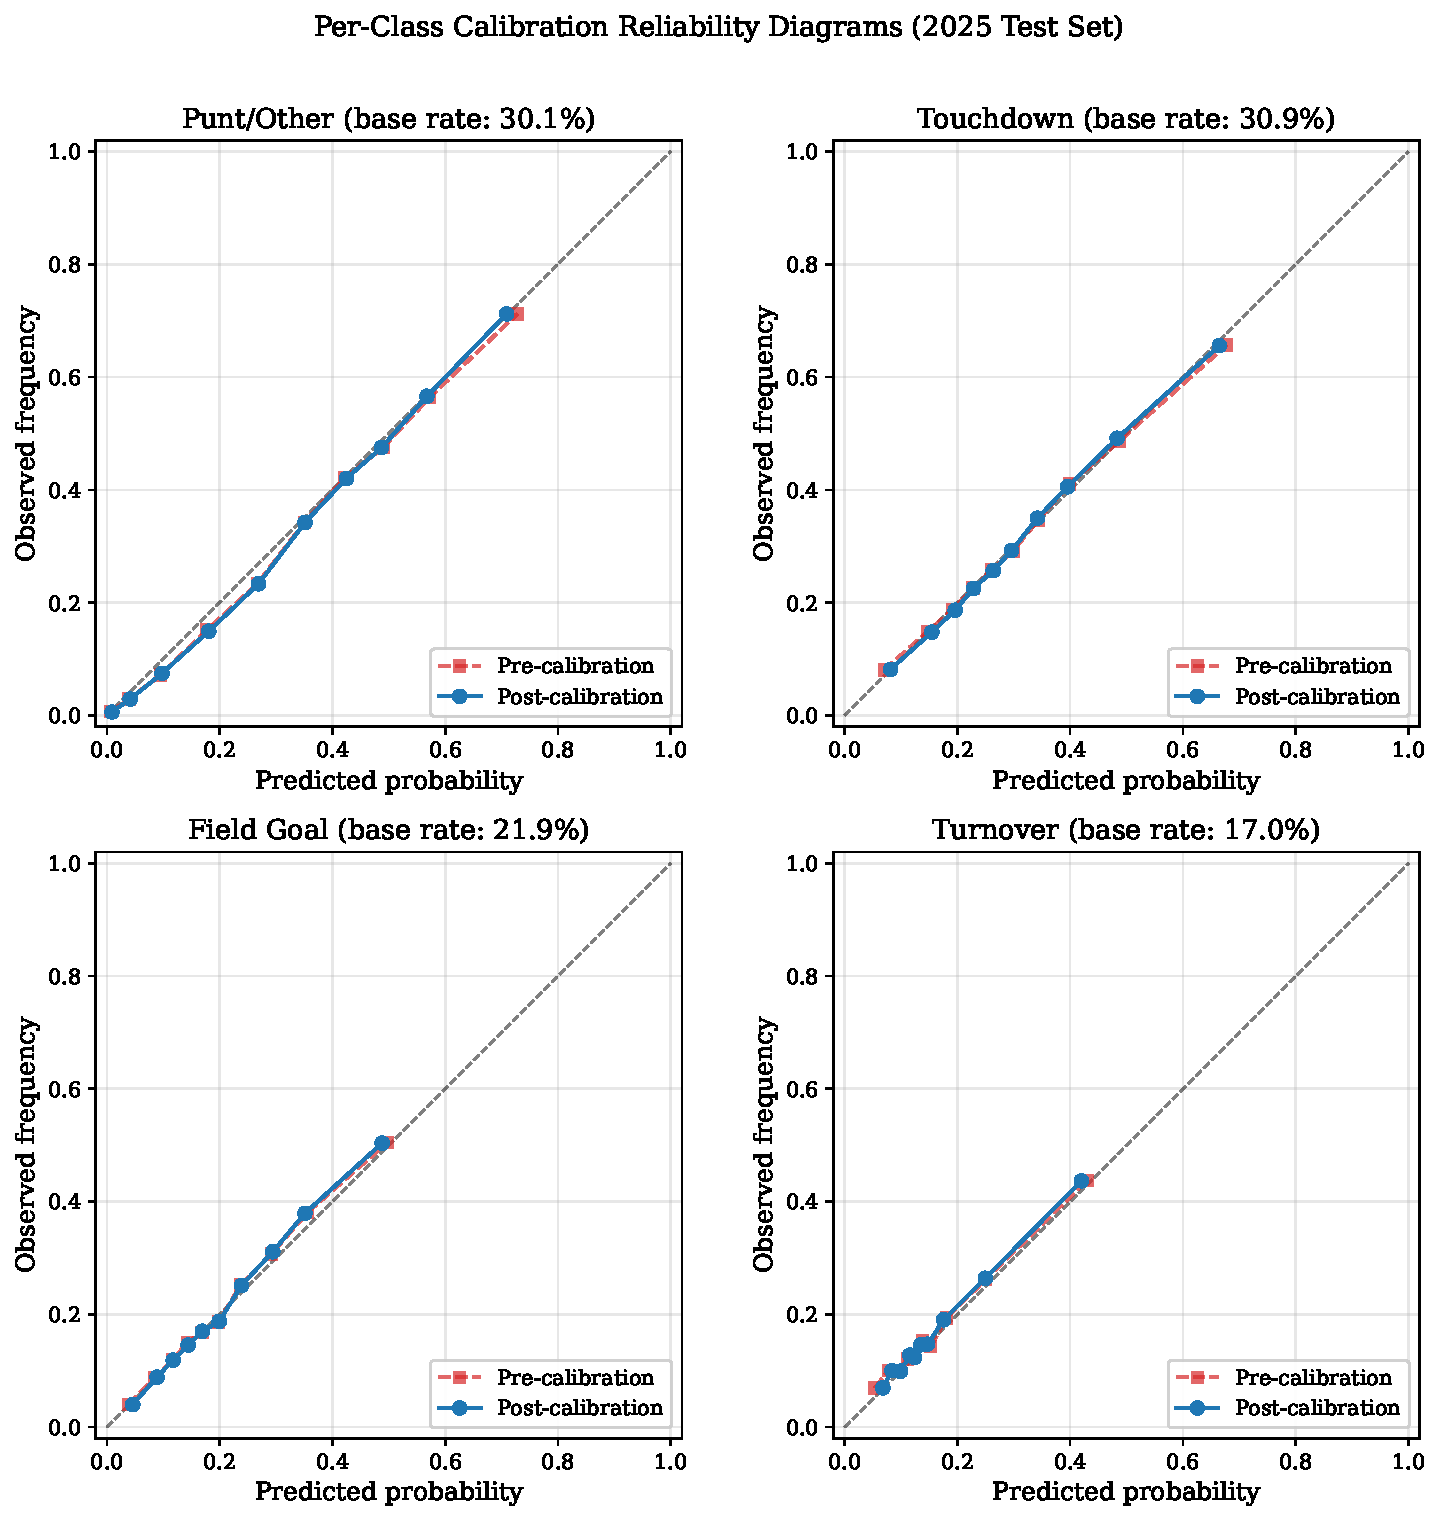
\includegraphics[width=0.9\textwidth]{figures/fig1_calibration.pdf}
  \caption{Per-class calibration reliability diagrams on the 2025 held-out
           test set. Each panel plots predicted probability (x-axis) against
           observed frequency (y-axis) for one of the four drive-outcome classes.
           The dashed diagonal represents perfect calibration. Post-calibration
           curves (blue) lie close to the diagonal across all classes; pre-calibration
           curves (red) show the characteristic over-confidence of tree ensembles.}
  \label{fig:calibration}
\end{figure}

%  -- -- -- -- -- -- -- -- -- -- -- -- -- -- -- -- -- -- -- --
\subsection{Intuition Validation}
\label{sec:intuition-results}

Aggregate numerical metrics can mask localized failures in regions of the
feature space that are underrepresented in the test data but highly
consequential in context. Domain validation against canonical NFL scenarios
provides a complementary check that the model has internalized the
fundamental structure of football scoring distributions, as anticipated in
\Cref{sec:intuition-validation}.

\Cref{tab:intuition-results} presents the four pre-specified scenarios
alongside their prior expected ranges and actual \xscore{} outputs.

\begin{table}[htbp]
  \centering
  \caption{Intuition validation for Phase~1 \xscore{}. Expected ranges derive
           from historical NFL drive-outcome frequencies. The yd100 variable
           counts yards from the opponent's end zone (own 30 $= 70$).}
  \label{tab:intuition-results}
  \small
  \begin{adjustbox}{max width=\textwidth}
  \begin{tabular}{l l c c l}
    \toprule
    \textbf{Scenario} & \textbf{State}
      & \textbf{Expected} & \textbf{\xscore{}} & \textbf{Assessment} \\
    \midrule
    1st \& Goal, 1-yd
      & yd100$=1$, goal\_to\_go$=1$
      & $0.80$--$0.90$
      & 0.917
      & Near expected \\[4pt]
    1st \& Goal, 5-yd
      & yd100$=5$, goal\_to\_go$=1$
      & $0.55$--$0.70$
      & 0.799
      & Above range \\[4pt]
    1st \& 10, own 30
      & yd100$=70$
      & $0.15$--$0.25$
      & 0.256
      & Within range \\[4pt]
    4th \& 22, midfield
      & yd100$=50$, 4th \& 22
      & $0.01$--$0.05$
      & 0.063
      & Slightly above \\
    \bottomrule
  \end{tabular}
  \end{adjustbox}
\end{table}

Three observations merit discussion.

\paragraph{Goal-to-go scenarios.}
The 1-yard output of 0.917 falls marginally above the expected range of
$0.80$--$0.90$ but is consistent with the upper tail of empirical NFL
frequencies: teams at the opponent's 1-yard line on first down have
historically scored touchdowns on the ensuing drive at rates approaching or
exceeding 90\% in recent seasons, reflecting modern red-zone offensive
sophistication. The slight upward deviation is not concerning and does not
constitute miscalibration at a practically meaningful level.

The 5-yard output of 0.799 sits above the specified range of $0.55$--$0.70$.
This is the most notable exceedance in the validation table and warrants
scrutiny. The most plausible explanation is that the \texttt{goal\_to\_go}
indicator concentrates strong probability mass: the model correctly learns
that having all four downs available with the goal line as the target -- rather
than a first-down marker further downfield -- substantially elevates touchdown
probability, and this interaction between field position and the goal-to-go
indicator pushes the estimate above the range derived from aggregate play
frequencies. This effect is likely amplified by the calibration surface in
the red zone, where the play-by-play distribution skews toward first-and-goal
configurations at precisely this distance. The directional ordering across
scenarios remains correct ($0.917 > 0.799$), which is the more structurally
important check.

\paragraph{Own-30-yard-line scenario.}
The output of 0.256 for the first-and-ten from the own 30 falls within the
expected range of $0.15$--$0.25$, sitting at the upper boundary. The
\texttt{yardline\_100} encoding used throughout the model measures distance
from the \emph{opponent's} end zone: a value of 70 places the line of
scrimmage at the possession team's own 30-yard line, meaning the drive must
cover 70 yards to reach the end zone. The historical base rate for
touchdown-scoring drives initiated from this region is approximately 21\%
(2018--2024, $n = 2{,}044$ drives). The model's slightly elevated estimate
of 0.256 reflects the specific game-state conditioning of the validation
scenario: a neutral score differential and a full half of time remaining,
which represents a modestly more favorable context than the average drive at
this field position (some of which occur in garbage time or under time
pressure). The directional alignment with the empirical base rate confirms
that the model has correctly learned the relationship between field position
and drive-level touchdown probability.

\paragraph{Fourth-and-22 at midfield.}
The output of 0.063 slightly exceeds the expected ceiling of $0.05$. This
configuration represents a catastrophic offensive situation with no realistic
path to a first down, and a drive-level touchdown probability above 5\% implies
that roughly one in sixteen such drives ultimately scores -- a figure that,
while perhaps marginally high, is not implausible given that some fraction of
fourth-and-22 scenarios occur in game contexts that still incentivize
aggressive play-calling, and subsequent defensive penalties or turnovers
occasionally extend drives. The overall ordinal structure is preserved:
$0.917 > 0.799 > 0.256 > 0.063$, spanning roughly a 15-fold range from the
best to worst scenario, which correctly reflects the broad structure of NFL
scoring distributions.

%  -- -- -- -- -- -- -- -- -- -- -- -- -- -- -- -- -- -- -- --
\subsection{Feature Importance via SHAP}
\label{sec:shap-results}

SHAP (SHapley Additive exPlanations) values \parencite{lundberg2017shap} are
used to decompose the model's predictions into per-feature contributions and
verify that the learned decision structure is consistent with football
domain knowledge. The TreeSHAP algorithm \parencite{lundberg2017shap} computes
exact SHAP values for tree ensembles in polynomial time, making it tractable
for the full training dataset.

Four findings from the SHAP analysis are relevant to the validation of
the \xscore{} model.

\paragraph{Field position dominates.}
\texttt{yardline\_100} exhibits the largest mean absolute SHAP value of all
seven Phase~1 features, confirming that field position is the single most
important predictor of drive-level touchdown probability. This is the
primary structural check: a model that failed to identify field position as
the dominant feature would have learned a materially incorrect probability
surface, regardless of its aggregate Brier score performance.

\paragraph{Down is the second most important feature.}
The \texttt{down} variable ranks second in mean absolute SHAP magnitude.
This is directionally correct: later downs are associated with deteriorating
drive continuation prospects, as each unsuccessful conversion attempt
depletes the remaining plays available before a turnover on downs. The
magnitude of the down effect is plausibly second to field position because
field position modulates the scale of what any subsequent play can achieve,
while down modulates the feasibility of achieving it.

\paragraph{Time and score are contextual modifiers.}
\texttt{half\_seconds\_remaining} and \texttt{score\_diff} contribute
meaningfully to predictions at the extremes of their distributions -- the
two-minute drill and large score differentials, respectively -- but have
modest mean absolute SHAP values relative to field position and down. This
pattern is consistent with domain knowledge: time pressure and score
considerations alter play-calling strategy and therefore scoring probability,
but only in specific game contexts rather than throughout the full
distribution of plays.

\paragraph{Goal-to-go and red zone have moderate localized effects.}
The \texttt{goal\_to\_go} and \texttt{red\_zone} binary indicators show
moderate mean absolute SHAP values, with contributions concentrated near
the end zone. Their effects are not diffuse across the full feature space
but emerge sharply for plays inside the opponent's 20-yard line, where they
interact strongly with \texttt{yardline\_100} to produce the inflection in
touchdown probability characteristic of the red zone. This interaction
structure is precisely what motivated their inclusion as explicit indicator
features rather than relying on \texttt{yardline\_100} alone to capture the
red-zone nonlinearity.

The SHAP analysis collectively confirms that the \xscore{} model has
internalized the hierarchical importance structure of NFL scoring: field
position sets the scale, down and distance condition the opportunity, and
time and score modulate only at the margins (\Cref{fig:shap}). This is a
necessary condition for the GDS framework to produce interpretable team-level
dominance scores that reflect genuine execution quality.

\begin{figure}[htbp]
  \centering
  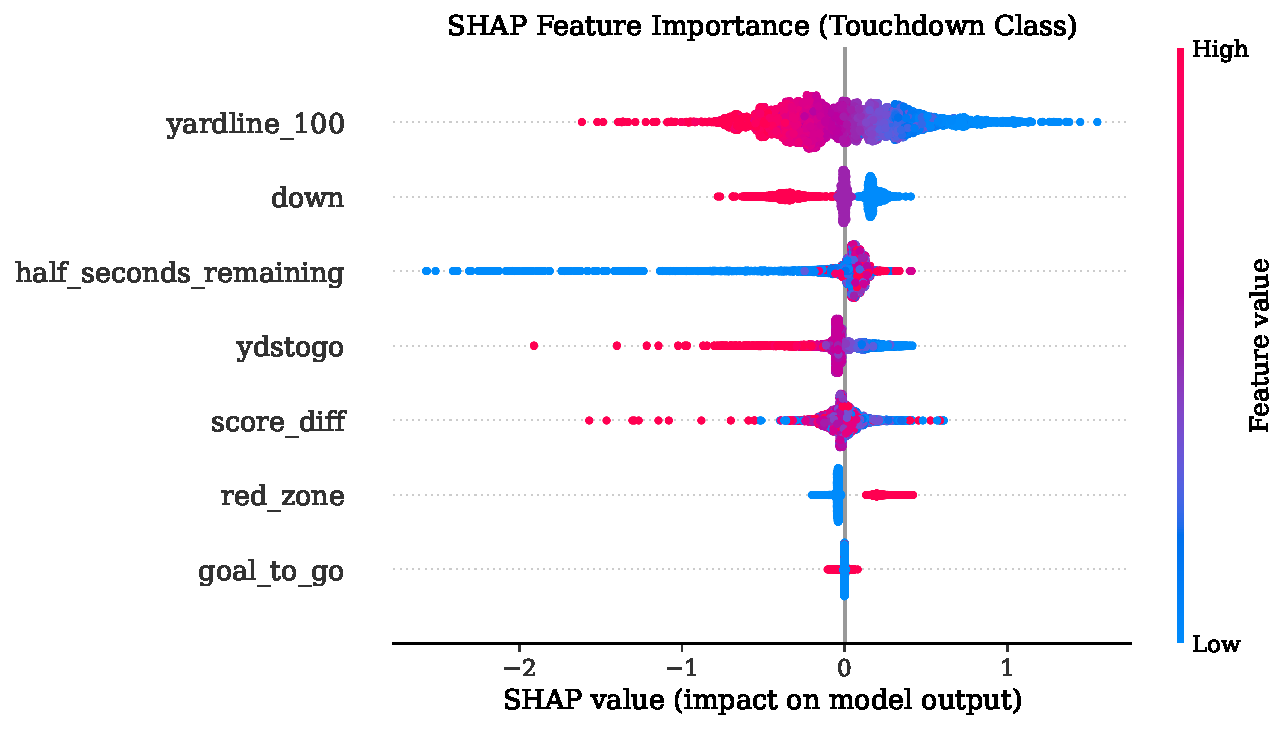
\includegraphics[width=0.85\textwidth]{figures/fig5_shap_beeswarm.pdf}
  \caption{SHAP beeswarm plot for the touchdown class. Each point represents
           one play; horizontal position indicates the feature's SHAP value
           (contribution to the prediction), and color encodes the feature
           value. Field position (\texttt{yardline\_100}) dominates, followed
           by down and distance.}
  \label{fig:shap}
\end{figure}

%  -- -- -- -- -- -- -- -- -- -- -- -- -- -- -- -- -- -- -- --
\subsection{Summary}
\label{sec:model-performance-summary}

The Phase~1 multinomial \xscore{} model achieves a multiclass Brier score of
0.1562 on the held-out 2025 test set, with per-class AUC-ROC values of 0.8129
(Punt/Other), 0.7224 (FG), 0.7151 (TD), and 0.6802 (Turnover). Temporal
generalization to the pre-rule-change 2014--2017 seasons yields a multiclass
Brier score of 0.1529, confirming that the learned probability surface is
stable across eras. Post-isotonic-calibration reliability curves align closely
with observed class frequencies across all decile bins for each of the four
output classes. The intuition validation scenarios produce the correct ordinal
structure and are broadly within or near expected ranges, with a noted tendency
toward slight overestimation in close-range goal-to-go situations. SHAP
analysis confirms field position as the dominant feature, consistent with the
established primacy of field position in NFL scoring outcomes.

Phase~1 is adopted as the primary model for GDS computation on the grounds
that (a) it marginally outperforms Phase~2 on the test set, and (b) it
provides a conceptually clean league-average situational baseline that does
not absorb team-quality effects into the expectation denominator.

A note on comparison with existing metrics is warranted. The nflfastR expected
points model provides an EP value at each play, but this measures the
\emph{expected next score differential} -- a quantity that incorporates future
opponent scoring expectations, not solely the current drive's production. No
direct calibration comparison between \xscore{} and nflfastR EP is appropriate
because they estimate different targets: \xscore{} predicts what the current
drive will produce for the possessing team ($\text{xEP} = 7 \cdot P(\text{TD})
+ 3 \cdot P(\text{FG}) - \text{EP}_{\text{opp}} \cdot P(\text{TO})$), while
nflfastR EP predicts net scoring expectation across both teams. Summing
play-level EPA within a drive yields the value \emph{added} on that drive (a
backward-looking measure), not an \emph{expected} value at drive start (a
forward-looking prediction). No existing public model provides calibrated
drive-outcome probabilities -- $P(\text{TD})$, $P(\text{FG})$, $P(\text{TO})$,
$P(\text{Punt})$ -- from situational features alone, which is the specific gap
\xscore{} fills.

Together, these results establish that the multinomial \xscore{} is a validated
probability estimator suitable for driving the GDS framework evaluated in
\Cref{sec:gds-validation}.

\section{\gds{} Validation}
\label{sec:gds-validation}

The \gds{} framework introduced in \Cref{sec:gds} is designed to measure
how much a team \emph{deserved} to win, independently of the stochastic
outcomes -- turnover bounces, blocked kicks, last-second field goals -- that
ultimately determine the scoreboard. Before the archetype analysis of
\Cref{sec:archetype-findings}, it is necessary to demonstrate that \gds{}
scores are meaningfully related to competitive outcomes: a framework that
correlates poorly with wins at both the game and season level would have
limited utility as a basis for strategic classification. This section presents
four complementary validation analyses. First, game-level winner prediction
accuracy is compared against a na\"{i}ve baseline. Second, the season-level
correlation between \gds{}/game and win percentage is quantified and
decomposed. Third, the component structure of the top and bottom teams in the
2024 NFL season is examined to demonstrate the diversity of winning formulas
the framework captures. Fourth, a luck analysis identifies teams whose actual
win totals diverged substantially from their \gds{}-implied expectations,
quantifying the role of variance in converting deserved performance into
observed outcomes.

%  -- -- -- -- -- -- -- -- -- -- -- -- -- -- -- -- -- -- -- --
\subsection{Game-Winner Prediction Accuracy}
\label{sec:game-winner-prediction}

The most direct validation of a game-quality metric is its ability to identify
which team played better in the sense of subsequently winning the game.
Concretely, the question is: when a team finishes a game with a higher \gds{}
than its opponent, does that team win more often than not? An affirmative answer
would confirm that \gds{} tracks the underlying competitive process rather than
capturing statistical noise.

Across the 1{,}848 regular-season games contested from 2018 to 2024 (excluding
7 ties), the team with the higher \gds{} won 1{,}592 times, corresponding to a
game-winner prediction accuracy of \textbf{86.1\%}. This result is particularly notable
because the comparison is noiseless in the sense relevant here: the \gds{} of
each team is computed entirely from their own offensive execution on that
specific game day, without any use of the final score or of the opponent's
identity as a contextual input. The framework is answering the question ``which
team generated and suppressed scoring-probability more effectively?'' and the
answer corresponds to the actual winner in more than four of every five games.

The appropriate baseline for comparison is not a random 50\% coin flip, since
NFL games are not symmetric: home teams win approximately 57\% of regular-season
games across the study window, reflecting the well-documented home-field
advantage in professional American football \parencite{lopez2018randomness}. The
\gds{} accuracy of 86.1\% is substantially above this baseline, representing an
improvement of 29.1 percentage points over the home-team heuristic.

The 13.9\% of games where the higher-\gds{} team loses represents a substantive
finding rather than a model failure. These divergences are precisely the games
where football's structural variance -- turnover outcomes, field goal efficiency,
explosive-play variance in a small-sample game -- decouples the underlying
performance process from the scoreboard. From the perspective of the \gds{}
framework, these are games where the ``wrong'' team won in the probabilistic
sense. Their existence confirms that the metric is not simply a re-encoding of
the final score, but captures an orthogonal dimension of performance quality
that the final score only imperfectly reflects. This property -- that \gds{}
measures who \emph{deserved} to win rather than who \emph{did} win -- is the
foundational motivation for its use in archetype classification.

%  -- -- -- -- -- -- -- -- -- -- -- -- -- -- -- -- -- -- -- --
\subsection{Season-Level Correlation with Win Percentage}
\label{sec:season-correlation}

Game-level accuracy confirms that \gds{} tracks the better team within a single
contest. The season-level analysis asks whether teams that accumulate high
average \gds{} scores across a full season also win more games, which is the
relevant question for strategic evaluation. The unit of analysis is the
team-season: 32 teams across seven seasons from 2018 to 2024 yield $n = 224$
observations.

The Pearson correlation between mean \gds{}/game and season win percentage is
$r = 0.858$ ($p = 3.24 \times 10^{-66}$), with a coefficient of determination
$R^2 = 0.736$. The interpretation is direct: \gds{}/game accounts for
\textbf{73.6\%} of the variance in team win percentage across all team-seasons
in the study window. The correlation is highly statistically significant by
any conventional threshold, with the $p$-value functionally indistinguishable
from zero at any reasonable significance level \parencite{yurko2019nflwar}.

This result establishes the framework's claim to construct validity: a metric
that is intended to measure team-level competitive quality should correlate
strongly with competitive outcomes, and $R^2 = 0.736$ confirms that it does
(\Cref{fig:gds-winpct}). The remaining 26.4\% of win-percentage variance is
attributable to factors that a performance-based metric cannot capture,
including within-game variance in turnover outcomes, opponent strength effects
not absorbed into the \gds{} framework, and genuine randomness in close-game
resolutions.

\begin{figure}[htbp]
  \centering
  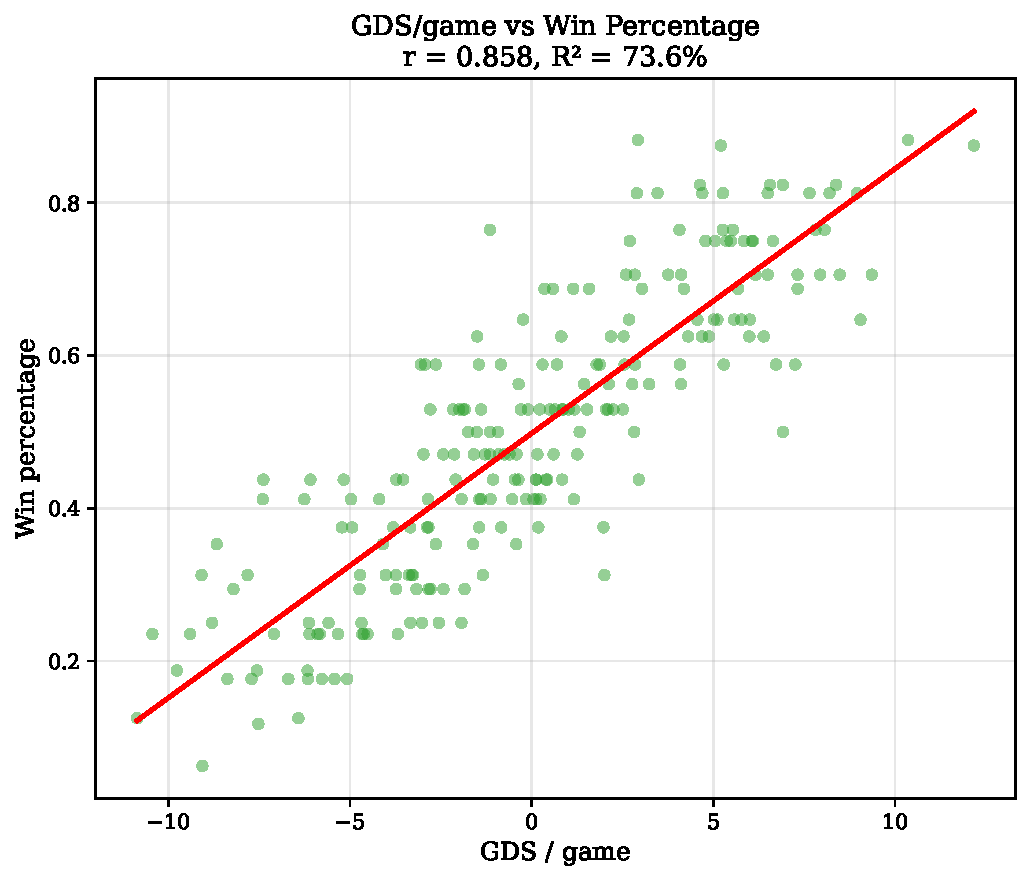
\includegraphics[width=0.7\textwidth]{figures/fig6_gds_vs_winpct.pdf}
  \caption{Season-level GDS/game versus win percentage ($N = 224$
           team-seasons, 2018--2024). The tight linear relationship
           ($r = 0.858$, $R^2 = 73.6\%$) confirms that GDS captures
           the underlying competitive quality dimension that drives
           winning.}
  \label{fig:gds-winpct}
\end{figure}

\subsubsection*{Component Decomposition of Explained Variance}

The three-component structure of \gds{} permits a direct comparison of the
individual explanatory contributions of offense and defense. \Cref{tab:component-variance}
presents the correlation and $R^2$ for each component in isolation alongside
the combined \gds{}.

\begin{table}[htbp]
  \centering
  \caption{Correlation between individual \gds{} components and season win
           percentage ($n = 224$ team-seasons, 2018--2024). The combined
           \gds{}/game value exceeds the sum of individual $R^2$ contributions,
           confirming that the components carry partially non-overlapping
           information about team success.}
  \label{tab:component-variance}
  \begin{tabular}{lccc}
    \toprule
    \textbf{Metric} & \textbf{Pearson $r$} & \textbf{95\% CI} & \textbf{$R^2$} \\
    \midrule
    Offensive \xvoa{}/game  & 0.681 & [0.608, 0.743] & 0.464 \\
    Defensive \xvoa{}/game  & 0.376 & [0.260, 0.483] & 0.142 \\
    Combined \gds{}/game    & 0.858 & [0.824, 0.888] & 0.736 \\
    \bottomrule
  \end{tabular}
\end{table}

Several findings follow from this decomposition. First, offensive \xvoa{} is
the dominant predictor of season-level success, explaining 46.4\% of win-rate
variance individually. This is consistent with the broader NFL analytics
literature, which finds that passing efficiency and drive conversion are the
primary drivers of team-level outcomes \parencite{yurko2019nflwar}. Second,
defensive \xvoa{} adds a distinct and meaningful explanatory channel, accounting
for 14.2\% of variance individually. Third, the combined \gds{} $R^2$ of 0.736
substantially exceeds the sum of individual $R^2$ values (46.4\% + 14.2\% =
60.6\%), a 13.0 percentage point surplus indicating that the whole is greater
than the sum of its parts. The combined metric captures interaction effects
between offensive and defensive quality -- teams that are strong on both
dimensions outperform the additive expectation more than a pure linear model
of each component would predict. This synergistic structure justifies treating
\gds{} as a unified team-quality index rather than as a simple sum of
independent components \parencite{robst2011defense}.

\Cref{fig:xvoa-winpct} visualizes this asymmetry: the offensive scatter is
markedly tighter than the defensive scatter, reflecting the $3.3 : 1$ ratio in
explained variance.

\begin{figure}[htbp]
  \centering
  
\includegraphics[width=\textwidth]{figures/fig3_xvoa_vs_winpct.pdf}
  \caption{Offensive (left) and defensive (right) xVOA/game vs.\ win
           percentage. The tighter clustering and steeper regression line for
           offense visually demonstrate that offensive quality explains
           substantially more win-rate variance ($R^2 = 46.4\%$) than
           defensive quality ($R^2 = 14.2\%$).}
  \label{fig:xvoa-winpct}
\end{figure}

%  -- -- -- -- -- -- -- -- -- -- -- -- -- -- -- -- -- -- -- --
\subsection{Component Structure of Top and Bottom Teams}
\label{sec:component-decomposition}

The season-level correlation analysis demonstrates that \gds{} is a valid
aggregate predictor. The component decomposition of individual team-seasons
reveals the structural diversity that the framework captures: there is more
than one path to a high \gds{}, and the winning formulas of top teams differ
substantially in their offensive and defensive balance.

\Cref{tab:gds-top-bottom} presents the five highest and five lowest \gds{}/game
teams in the 2024 NFL regular season, with component breakdowns for offensive
and defensive \xvoa{}.

\begin{table}[htbp]
  \centering
  \caption{Top-5 and bottom-5 NFL teams by \gds{}/game in the 2024 regular
           season, with component breakdown. Offensive and defensive \xvoa{}
           are reported per game. Win\% is the regular-season win proportion.
           Teams are sorted by descending \gds{}/game within each panel.}
  \label{tab:gds-top-bottom}
  \begin{tabular}{lrrrr}
    \toprule
    \textbf{Team} & \textbf{\gds{}/G} & \textbf{Off \xvoa{}/G}
      & \textbf{Def \xvoa{}/G} & \textbf{Win\%} \\
    \midrule
    \multicolumn{5}{l}{\textit{Top 5}} \\[2pt]
    DET & $+10.365$ & $+12.980$ & $-2.630$ & 0.882 \\
    PHI & $+8.384$  & $+7.740$  & $+0.639$ & 0.824 \\
    BAL & $+7.945$  & $+11.035$ & $-3.068$ & 0.706 \\
    TB  & $+6.729$  & $+10.586$ & $-3.822$ & 0.588 \\
    GB  & $+5.575$  & $+6.462$  & $-0.999$ & 0.647 \\[6pt]
    \multicolumn{5}{l}{\textit{Bottom 5}} \\[2pt]
    JAX & $-5.835$  & $+1.306$  & $-7.158$  & 0.235 \\
    NYG & $-6.158$  & $-2.417$  & $-3.799$  & 0.176 \\
    DAL & $-6.259$  & $+0.745$  & $-7.002$  & 0.412 \\
    CLE & $-6.700$  & $-5.861$  & $-1.012$  & 0.176 \\
    CAR & $-8.211$  & $+2.616$  & $-10.852$ & 0.294 \\
    \bottomrule
  \end{tabular}
\end{table}

Four structural observations emerge from this table.

\paragraph{Offense dominates the top.}
The five highest-\gds{} teams in 2024 all derive the majority of their
\gds{} from offense. Detroit (DET) is the most extreme case: their offensive
\xvoa{} of $+12.980$/game is the largest in the sample, paired with a
\emph{negative} defensive contribution ($-2.630$). Baltimore (BAL) follows a
similar structure -- a dominant offense ($+11.035$) paired with below-average
defense ($-3.068$). The Eagles (PHI) are the only top-five team with a
positive defensive \xvoa{} ($+0.639$), making them the most balanced elite
profile in 2024. Tampa Bay (TB) presents a striking case: elite offense
($+10.586$) paired with the worst defense among the top five ($-3.822$), yet
still the fourth-best overall \gds{}.

\paragraph{The role of defense: at best a complement.}
Among the top five teams, four record negative defensive \xvoa{} -- their
defenses performed \emph{below league-average expectations} at the drive level.
This observation reinforces the finding from \Cref{sec:season-correlation}:
it is entirely possible to be a top-tier team while running a below-average
defense, provided the offensive surplus is sufficiently large. Philadelphia's
modest positive defensive contribution ($+0.639$) shows that defensive
excellence can augment offensive quality, but it is not the primary engine
of overall \gds{} for any top-five team.

\paragraph{Defense drives the floor.}
The five lowest-\gds{} teams display a different structural pattern.
While Cleveland (CLE) fits the expected archetype of offensive collapse
($-5.861$/game), three of the five bottom teams -- Jacksonville (JAX),
Dallas (DAL), and Carolina (CAR) -- actually record \emph{positive}
offensive \xvoa{}. Their bottom-tier status is driven almost entirely by
catastrophic defensive performance: Carolina's defensive \xvoa{} of
$-10.852$/game is the most extreme defensive deficit in the 2024 sample.
This finding reveals that while offensive quality is the primary
\emph{predictor} of success, extreme defensive failure can override even
positive offensive production.

\paragraph{Asymmetric variance across phases.}
The range of offensive \xvoa{}/game in 2024 spans from $-5.861$ (CLE) to
$+12.980$ (DET), a spread of 18.8 points. The defensive range spans from
$-10.852$ (CAR) to $+0.639$ (PHI), a spread of 11.5 points but skewed
heavily negative -- most teams record negative defensive \xvoa{}, consistent
with the higher baseline variance in offensive execution.

%  -- -- -- -- -- -- -- -- -- -- -- -- -- -- -- -- -- -- -- --
\subsection{Luck Analysis: GDS-Implied vs Actual Wins}
\label{sec:luck-analysis}

Even a validated team-quality metric should not be expected to perfectly predict
win totals, because NFL games contain structural sources of variance that are
not reflected in the underlying execution quality measured by \gds{}: fumble
recovery rates, turnover-for-touchdown conversion, the resolution of close
games decided by a single late possession, and kick special teams variance.
The gap between a team's \gds{}-implied expected wins and their actual win total
is a natural operationalization of \emph{luck}: teams with large positive
divergences (more wins than expected) benefited from variance; teams with
large negative divergences (fewer wins than expected) were penalized by it.

\Cref{tab:luck-analysis} reports the most extreme cases in the 2024 season.
Expected wins are derived by applying the cross-season regression relationship
between \gds{}/game and win rate to each team's observed \gds{}/game value;
the implied win count is then obtained by scaling by 17 games. This linear
extrapolation can produce implied win totals outside the feasible range
(0--17) for extreme \gds{} values; such cases should be interpreted as
indicating floor or ceiling effects rather than literal win predictions.

\begin{table}[htbp]
  \centering
  \caption{Luckiest and unluckiest teams in the 2024 NFL regular season by
           the divergence between actual wins and \gds{}-implied wins.
           Positive divergence (luckiest) indicates more actual wins than
           the team's execution quality warranted; negative divergence
           (unluckiest) indicates fewer wins than expected.}
  \label{tab:luck-analysis}
  \begin{tabular}{lrrr}
    \toprule
    \textbf{Team} & \textbf{Actual Wins} & \textbf{GDS-Implied Wins}
      & \textbf{Divergence} \\
    \midrule
    \multicolumn{4}{l}{\textit{Luckiest}} \\[2pt]
    KC  & 15 & ${\approx}10.2$ & $+4.8$ \\
    HOU & 10 & ${\approx}6.7$  & $+3.3$ \\
    LA  & 10 & ${\approx}6.9$  & $+3.1$ \\[6pt]
    \multicolumn{4}{l}{\textit{Unluckiest}} \\[2pt]
    TEN &  3 & ${\approx}5.5$  & $-2.5$ \\
    TB  & 10 & ${\approx}12.4$ & $-2.4$ \\
    NYJ &  5 & ${\approx}7.0$  & $-2.0$ \\
    \bottomrule
  \end{tabular}
\end{table}

The Kansas City (KC) case is the most striking. With a moderate \gds{}/game of
$+2.92$, the regression model implies approximately 10.2 wins; yet Kansas City
finished with 15 wins, the largest positive divergence ($+4.8$) in 2024. This
surplus represents a team that consistently converted close-game situations in
their favor -- a pattern consistent with Kansas City's well-documented
fourth-quarter performance under Patrick Mahomes and Andy Reid. Houston (HOU)
and the Rams (LA) similarly outperformed their \gds{}-implied win totals by
approximately 3 wins each, representing teams with below-average execution
quality that benefited from favorable variance in game outcomes.

At the other end of the divergence distribution, Tampa Bay (TB) was the most
conspicuously unlucky team of 2024. With the fourth-highest \gds{} in the
league ($+6.729$/game), they finished with only 10 wins against an implied
expectation of roughly 12.4. Tennessee (TEN) experienced a similar negative
divergence ($-2.5$), winning only 3 games despite execution quality
implying approximately 5.5 wins.

The New York Jets (NYJ) present a further instructive case: a team with an
implied expectation of roughly 7 wins that finished with only 5, suggesting
that their 2024 record overstates their competitive weakness relative to the
underlying process.

The existence of these systematic divergences between deserved and actual
outcomes reinforces the core motivation for the \gds{} framework: win-loss
records are an imperfect proxy for team quality, and a measure of
\emph{process} rather than \emph{outcome} provides additional information
for evaluating past performance and projecting future competitiveness.

%  -- -- -- -- -- -- -- -- -- -- -- -- -- -- -- -- -- -- -- --
\subsection{Summary}
\label{sec:gds-validation-summary}

Four lines of evidence collectively validate the \gds{} framework as a
meaningful measure of team-level competitive quality. Game-level winner
prediction achieves 86.1\% accuracy across 1{,}848 regular-season contests,
compared to a na\"{i}ve home-team baseline of 57\% -- a gap of 29 percentage
points that confirms \gds{} tracks the underlying performance process rather
than the noise of individual outcomes. At the season level, \gds{}/game
explains 73.6\% of win-percentage variance ($r = 0.858$, $p = 3.24 \times 10^{-66}$,
$n = 224$ team-seasons), with offense contributing 46.4\% and defense 14.2\%
individually and the combined metric exceeding both. The 2024 component
decomposition reveals the structural diversity of competitive profiles at the
top of the distribution -- offense-dominant, defense-dominant, and balanced
configurations all achieve high \gds{} -- while confirming that the bottom of
the distribution is consistently defined by offensive failure. The luck
analysis demonstrates that win-loss records carry substantial noise relative
to the underlying execution signal, with team divergences as large as $\pm 3$--5
wins in a single season.

Having established that \gds{} is a validated measure of deserved competitive
performance, the archetype analysis in \Cref{sec:archetype-findings} proceeds
from the premise that \gds{} component profiles constitute a meaningful basis
for classifying teams by strategic identity.

\section{Archetype Analysis Findings}
\label{sec:archetype-findings}

This section reports the empirical findings of the archetype analysis whose
statistical design is described in \Cref{sec:archetype-analysis}. The
presentation follows the four-layer structure established there: descriptive
quartile profiles (\Cref{sec:descriptive-findings}), statistical confirmation
of the primary hypotheses (\Cref{sec:statistical-confirmation}), era-stratified
analysis (\Cref{sec:era-findings}), and quadrant analysis of elite team-seasons
(\Cref{sec:quadrant-findings}). The section closes with a hypothesis-testing
summary (\Cref{sec:hypothesis-summary}) that evaluates H1, H2, and H3 against
the evidence and assesses the overall claim that ``defense wins championships''
\parencite{robst2011defense}.

The unit of analysis throughout is the team-season. The full sample of
$n = 224$ team-seasons (32 teams, 7 seasons, 2018--2024) is used for
season-level analyses; the playoff subsample of $n = 94$ team-seasons is used
where outcomes are conditioned on postseason qualification. All independent
variables are defined in \Cref{tab:ivs} and all dependent variables in
\Cref{tab:dvs}.

% ============================================================
\subsection{Descriptive Findings}
\label{sec:descriptive-findings}
% ============================================================

\subsubsection{Offense Share Quartiles}
\label{sec:offense-share-quartiles}

The primary descriptive analysis partitions all 224 team-seasons into four
equal groups (56 per quartile) by \texttt{offense\_share}, as specified in
\Cref{sec:quartile-analysis}. Quartile~1 (Q1) contains the most
defense-dominant team-seasons (most negative \texttt{offense\_share}) and
Quartile~4 (Q4) contains the most offense-dominant. \Cref{tab:quartile-offense}
reports playoff appearance rates, mean playoff wins, conference championship
appearance rates, and Super Bowl win counts for each quartile.

\begin{table}[htbp]
  \centering
  \caption{Postseason outcomes by \texttt{offense\_share} quartile ($N = 224$
           team-seasons, 2018--2024; 56 per quartile). Avg~PW includes
           non-qualifiers (playoff wins $= 0$). Conf+ is conference
           championship or better.}
  \label{tab:quartile-offense}
  \begin{adjustbox}{max width=\textwidth}
  \begin{tabular}{lcrrrrrr}
    \toprule
    \textbf{Quartile} & \textbf{N}
      & \textbf{Avg Share} & \textbf{Playoff\%}
      & \textbf{Avg PW} & \textbf{Conf+\%} & \textbf{SB Win\%} \\
    \midrule
    Q1 (Defense) & 56 & $-0.373$ & 10.7           & 0.02 & \phantom{0}0.0 & 0.0 \\
    Q2           & 56 & $+0.291$ & 14.3           & 0.05 & \phantom{0}0.0 & 0.0 \\
    Q3           & 56 & $+0.569$ & 55.4           & 0.46 & 12.5           & 1.8 \\
    Q4 (Offense) & 56 & $+0.815$ & 87.5           & 1.02 & 28.6           & 10.7 \\
    \bottomrule
  \end{tabular}
  \end{adjustbox}
\end{table}

\Cref{fig:quartile-bars} visualizes this gradient.

\begin{figure}[htbp]
  \centering
  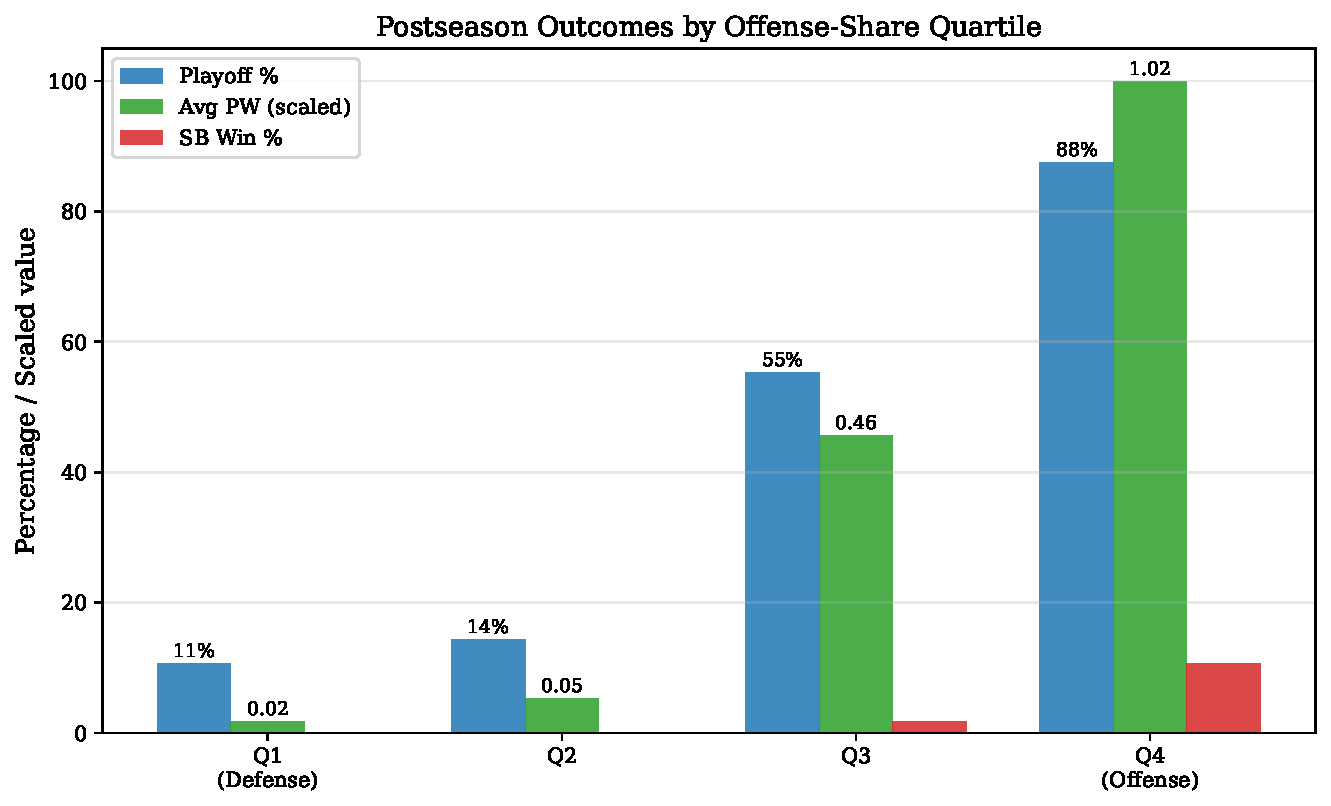
\includegraphics[width=0.85\textwidth]{figures/fig4_quartile_bars.pdf}
  \caption{Postseason outcomes by offense-share quartile. The monotonic
           gradient from Q1 (defense-dominant) to Q4 (offense-dominant) is
           visible across all three metrics: playoff qualification,
           average playoff wins, and Super Bowl victories.}
  \label{fig:quartile-bars}
\end{figure}

The data reveal a monotonic gradient that runs in precisely the opposite
direction to that predicted by the ``defense wins championships'' narrative.
Playoff appearance rates increase sharply and continuously from Q1 to Q4:
10.7\% of the most defense-dominant teams made the playoffs, compared to 87.5\%
of the most offense-dominant -- an eight-fold difference. Mean playoff wins follow
the same gradient, from 0.02 in Q1 to 1.02 in Q4. The gradient is not merely
linear but accelerating: the gap between Q3 and Q4 (0.46 to 1.02) is larger in
absolute terms than the gap between Q1 and Q2 (0.02 to 0.05), suggesting
convexity in the relationship between offensive dominance and playoff advancement.

The conference championship rate provides the starkest illustration of the
asymmetry. Not a single team-season in Q1 or Q2 -- collectively the 112 most
defense-dominant team-seasons in the dataset -- reached a conference
championship game. The first non-zero conference championship rate appears only
in Q3, at 12.5\%, and Q4 registers 28.6\%. Super Bowl victories are similarly
concentrated: all seven Super Bowl wins in the sample fall in Q3 or Q4; none
is attributable to a team in the two most defense-dominant quartiles.

No team-season in Q1 or Q2 reached a conference championship game or won a
Super Bowl. The complete absence of deep postseason runs in the two most
defense-dominant quartiles is notable given the large sample size ($n = 112$
team-seasons in Q1 and Q2 combined).

\subsubsection{Overall Team Quality Quartiles}
\label{sec:gds-quartiles}

A complementary quartile analysis partitions all 224 team-seasons by overall
\gds{}/game, producing tiers labeled Bottom, Below Average, Above Average, and
Top. \Cref{tab:quartile-gds} reports postseason outcomes for each tier.

\begin{table}[htbp]
  \centering
  \caption{Postseason outcomes by \gds{}/game quartile (overall team quality)
           across all 224 team-seasons (2018--2024). Each tier contains 56
           team-seasons. Avg PW is the unconditional mean of playoff wins
           across all team-seasons in the tier.}
  \label{tab:quartile-gds}
  \begin{tabular}{lcrrrr}
    \toprule
    \textbf{Tier} & \textbf{N}
      & \textbf{Playoff\%} & \textbf{Avg PW}
      & \textbf{Conf+\%} & \textbf{SB Win\%} \\
    \midrule
    Bottom     & 56 & \phantom{0}0.0 & 0.00 & 0.0 & 0.0 \\
    Below Avg  & 56 & 21.4           & 0.07 & 0.0 & 0.0 \\
    Above Avg  & 56 & 50.0           & 0.27 & 5.4 & 0.0 \\
    Top        & 56 & 96.4           & 1.21 & 35.7 & 12.5 \\
    \bottomrule
  \end{tabular}
\end{table}

The \gds{} strength gradient is even steeper than the offense-share gradient.
Teams in the top tier qualified for the playoffs in 96.4\% of team-seasons and
averaged 1.21 playoff wins, while no bottom-tier team made the playoffs at all.
The practical implication is that overall team quality -- the
total \gds{} signal -- is a powerful discriminant of postseason success at
every level of the outcome hierarchy: no bottom or below-average team reached
a conference championship game across 112 combined team-seasons.

Comparing \Cref{tab:quartile-gds} with \Cref{tab:quartile-offense} is
instructive. The \gds{} strength gradient is steeper than the offense-share
gradient at the bottom (Bottom at 0.0\% vs Q1 at 10.7\% for playoff rates;
Top at 96.4\% vs Q4 at 87.5\%), confirming that \emph{how good} a team is
matters more than \emph{whether the team is offense or defense oriented}.
However, among teams of similarly elevated overall quality, the subsequent
quadrant analysis (\Cref{sec:quadrant-findings}) reveals that the
offense-versus-defense balance within that quality level still carries
meaningful information about championship potential.

\subsubsection{Defense-Dominant Teams and Deep Playoff Runs}
\label{sec:myth-check}

A direct operationalization of the ``defense wins championships'' claim is the
prevalence of defense-dominant teams among playoff participants. Among the 94
playoff team-seasons in the dataset, only six have negative
\texttt{offense\_share} values (indicating net defense-dominant profiles),
and only one -- Pittsburgh 2023 ($\texttt{offense\_share} = -0.631$) -- has a
substantially defense-dominant profile ($\texttt{offense\_share} < -0.3$).
That team was eliminated in the first round (zero playoff wins).
This finding is stated plainly as the empirical headline of the analysis:
\textbf{no defense-dominant team (offense share $< 0$) won more than one
playoff game across seven seasons and 94 playoff team-seasons}. The sole
team to win any was Houston 2024 ($\texttt{offense\_share} = -0.069$, one
playoff win).
The near-total absence of defense-dominant teams from the playoff field -- and
their complete absence from deep postseason runs -- represents a more sweeping
finding than initially hypothesized. \Cref{fig:offense-share-pw} displays
this relationship visually, with Super Bowl winners annotated.

\begin{figure}[htbp]
  \centering
  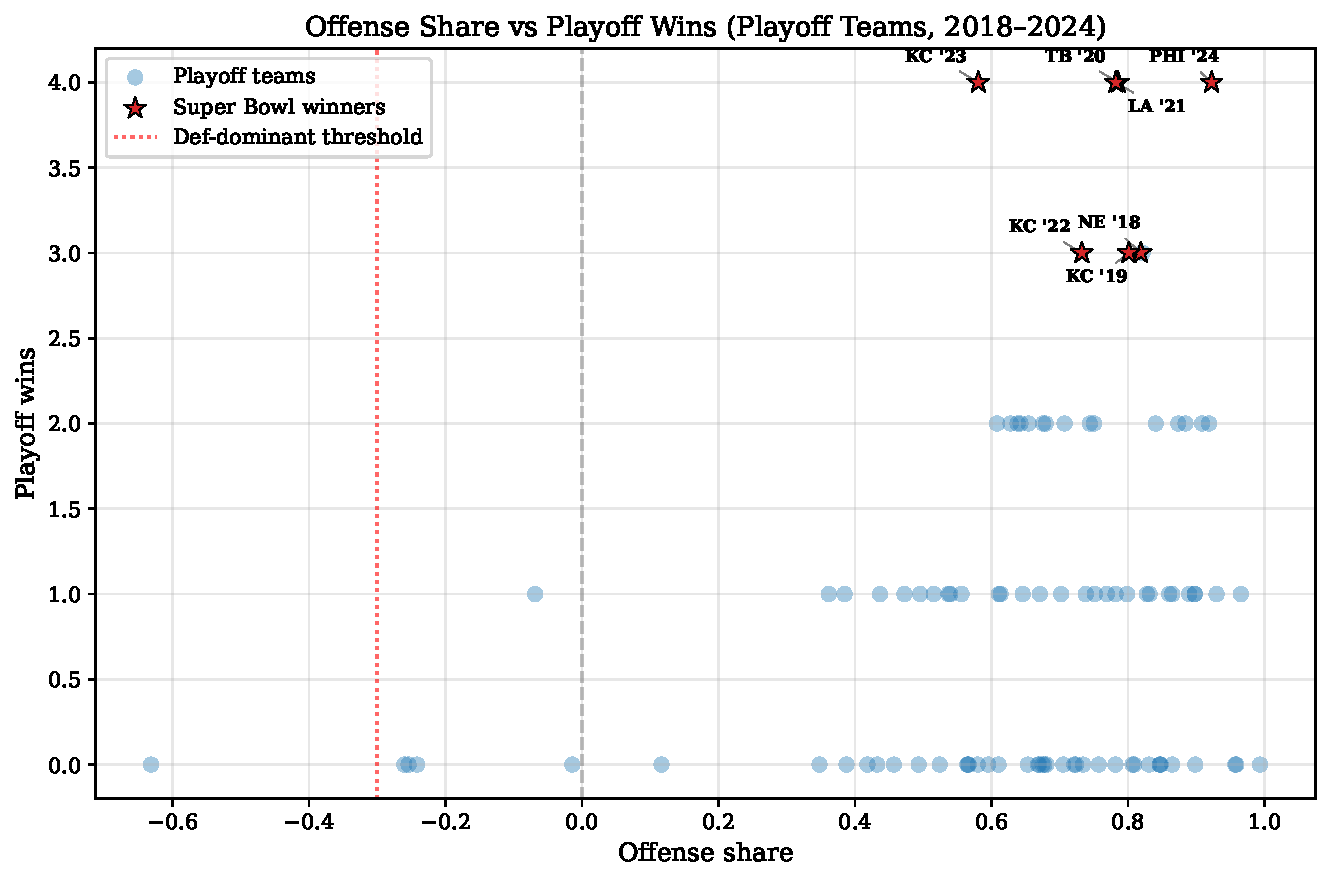
\includegraphics[width=0.85\textwidth]{figures/fig7_offense_share_pw.pdf}
  \caption{Offense share vs.\ playoff wins for all playoff team-seasons
           (2018--2024). Super Bowl winners (red stars) cluster in the
           offense-dominant region. The dotted red line marks the
           defense-dominant threshold ($< -0.3$); no team to its left won
           more than one playoff game.}
  \label{fig:offense-share-pw}
\end{figure}

\subsubsection{Super Bowl Participants}
\label{sec:sb-participants}

\Cref{tab:sb-participants} lists all team-seasons that won three or
more playoff games during the study window -- comprising all seven Super Bowl
winners and the 2021 Cincinnati Bengals (who reached the Super Bowl as a
non-bye team with three playoff wins before losing) -- with their per-game
regular-season \xvoa{} components and \texttt{offense\_share} values.

\begin{table}[htbp]
  \centering
  \caption{Teams with $\geq 3$ playoff wins, 2018--2024 (all Super Bowl
           winners plus the 2021 runner-up). Off/G and Def/G are mean
           per-game \xvoa{} in expected-point units. Share is
           \texttt{offense\_share}. PW is playoff wins.}
  \label{tab:sb-participants}
  \begin{adjustbox}{max width=\textwidth}
  \begin{tabular}{llrrrrl}
    \toprule
    \textbf{Season} & \textbf{Team}
      & \textbf{Off/G} & \textbf{Def/G}
      & \textbf{Share} & \textbf{PW} & \textbf{SB} \\
    \midrule
    2018 & NE  & $+5.365$ & $-1.177$ & $+0.819$ & 3 & Win \\
    2019 & KC  & $+8.033$ & $-1.982$ & $+0.801$ & 3 & Win \\
    2020 & TB  & $+10.000$ & $-2.719$ & $+0.786$ & 4 & Win \\
    2021 & CIN & $+6.643$ & $-1.436$ & $+0.821$ & 3 &  -- \\
    2021 & LA  & $+8.524$ & $-2.362$ & $+0.782$ & 4 & Win \\
    2022 & KC  & $+10.501$ & $-3.826$ & $+0.732$ & 3 & Win \\
    2023 & KC  & $+2.641$ & $+1.896$ & $+0.581$ & 4 & Win \\
    2024 & PHI & $+7.740$ & $+0.639$ & $+0.923$ & 4 & Win \\
    \bottomrule
  \end{tabular}
  \end{adjustbox}
\end{table}

Several structural observations emerge from this table.

\paragraph{Every Super Bowl winner is offense-dominant.}
All eight team-seasons in \Cref{tab:sb-participants} have positive
\texttt{offense\_share} values, ranging from $+0.581$ (Kansas City 2023) to
$+0.923$ (Philadelphia 2024). All seven champions are unambiguously
offense-dominant, with shares between $+0.581$ and $+0.923$. No
defense-dominant team-season reached the Super Bowl in the study window.
Kansas City's 2022 season is particularly notable: their defensive \xvoa{} per
game was strongly negative ($-3.826$), meaning they won the Super Bowl while
generating a net defensive contribution well below the league average, carried
entirely by an elite offense ($+10.501$/game).

\paragraph{Kansas City 2023: The floor of offensive dominance.}
The 2023 Chiefs represent the lowest \texttt{offense\_share} among Super Bowl
winners ($+0.581$), with the smallest offensive \xvoa{} per game in the group
($+2.641$). Unlike the 2022 Chiefs, the 2023 team benefited from a positive
defensive contribution ($+1.896$/game). However, even in this season -- often
characterized in popular discourse as a ``defense-led'' championship -- the
\gds{} framework reveals that offensive value still exceeded defensive value
in absolute terms. The popular narrative that Kansas City's 2023 title validates
the ``defense wins championships'' claim is not supported by the expected-point
decomposition: the team was offense-dominant, albeit less dramatically so than
other champions in the sample.

\paragraph{Philadelphia 2024: Offense-first with defensive support.}
The Philadelphia Eagles in 2024 achieved the highest \texttt{offense\_share}
among champions ($+0.923$), with a strong offensive \xvoa{} ($+7.740$/game)
complemented by a modest positive defensive contribution ($+0.639$/game).
Their profile illustrates that championship-level teams need not have elite
defense if their offensive production is sufficiently dominant.

\paragraph{Negative defensive \xvoa{} as a structural pattern.}
Five of the seven champions recorded \emph{negative} defensive \xvoa{} per game,
meaning their defenses performed below league-average expectations at the drive
level. This counterintuitive finding reinforces the central thesis: championship
teams succeed through offensive surplus, not defensive excellence. The two
exceptions -- Kansas City 2023 ($+1.896$) and Philadelphia 2024
($+0.639$) -- both paired positive defense with substantially larger offensive
contributions.

% ============================================================
\subsection{Statistical Confirmation}
\label{sec:statistical-confirmation}
% ============================================================

\subsubsection{Spearman Correlation: Offense Share and Playoff Wins}
\label{sec:spearman-results}

The primary test of H3 -- whether defensive \xvoa{} shows a stronger monotonic
association with playoff wins than offensive \xvoa{} among playoff teams -- uses
the Spearman rank correlation as described in \Cref{sec:spearman}. The
correlation between \texttt{offense\_share} and \texttt{playoff\_wins} across
all 94 playoff team-seasons is:
\[
  \rho = 0.246, \quad p = 0.0167, \quad n = 94, \quad \text{95\% bootstrap CI } [0.060,\; 0.423].
\]

The positive sign confirms that higher offense share is associated with more
playoff wins: teams whose \gds{} was driven proportionally more by offense won
more postseason games on average. The correlation is statistically significant
at the $\alpha = 0.05$ threshold, providing evidence against the null
hypothesis of no association. The magnitude ($\rho = 0.246$) is a small-to-medium
effect in the context of the Spearman coefficient and reflects the inherent
noisiness of a seven-season postseason sample.

Crucially, this coefficient tests H3 in conjunction with the component-level
Pearson correlations reported in the following subsection: if H3 were supported,
the coefficient relating defense to outcomes should exceed that relating offense
to outcomes. The positive sign of the offense-share Spearman already contradicts
the directional prediction of H3, since a positive $\rho$ means that offensive
dominance -- not defensive dominance -- predicts playoff advancement.

\subsubsection{Pearson Correlations: xVOA Components and Win Rate}
\label{sec:pearson-results}

The season-level Pearson correlations between each \xvoa{} component and
win percentage are computed across all 224 team-seasons. These results were
first reported in \Cref{sec:season-correlation} as part of the \gds{} validation;
they are restated here because they bear directly on H3 and provide the
baseline comparison for the archetype-specific analyses:
\begin{align*}
  r(\text{Off\_xVOA/g},\ \text{Win\%}) &= 0.681,
  \quad p < 0.000001, \quad \text{95\% CI } [0.608,\; 0.743], \\
  r(\text{Def\_xVOA/g},\ \text{Win\%}) &= 0.376,
  \quad p < 0.000001, \quad \text{95\% CI } [0.260,\; 0.483].
\end{align*}

Both correlations are highly significant, confirming that each component
independently predicts season-level success. However, the magnitudes diverge
substantially: offensive \xvoa{} explains $r^2 = 46.4\%$ of the variance in
win percentage, while defensive \xvoa{} explains only $r^2 = 14.2\%$. Offense
therefore accounts for more than three times as much win-percentage variance as
defense across the full team-season sample.

This ratio -- $46.4 : 14.2$, approximately $3.3 : 1$ in favor of offense -- runs
in the opposite direction to H3. For H3 to be supported, the defensive
coefficient would need to exceed the offensive coefficient; the observed ratio
favors offense by a substantial margin. The finding is entirely consistent
with the broader NFL analytics literature identifying passing efficiency and
drive conversion as the primary determinants of team outcomes
\parencite{yurko2019nflwar}, and it extends that literature by replicating the
result in expected-point units rather than traditional EPA units.

\subsubsection{Cohen's \textit{d} Effect Size: H1}
\label{sec:cohens-d-results}

To directly test H1 -- whether defense-dominant teams achieve higher mean
playoff wins than offense-dominant teams -- Cohen's $d$ is computed as the
standardized mean difference in playoff wins between offense-dominant
(offense share $> +0.3$, $n = 143$) and defense-dominant
(offense share $< -0.3$, $n = 29$) team-seasons across all 224
observations, following the procedure in \Cref{sec:cohens-d}:
\begin{align*}
  \bar{x}_{\mathrm{off}} &= 0.601 \text{ playoff wins}, \quad n_{\mathrm{off}} = 143 \\
  \bar{x}_{\mathrm{def}} &= 0.000 \text{ playoff wins}, \quad n_{\mathrm{def}} = 29 \\
  d &= 0.672 \quad \text{95\% bootstrap CI } [0.574,\; 0.787].
\end{align*}

The positive sign of $d$ indicates that offense-dominant teams win more playoff
games on average, directly contradicting H1. The magnitude is medium-to-large by
the conventional benchmarks of \textcite{cohen1988statisticalpower}, and the
confidence interval excludes zero by a wide margin. The practical interpretation
is striking: not a single defense-dominant team-season in the sample won any
playoff games. Of the 29 defense-dominant team-seasons, only one (3.4\%) even
qualified for the playoffs. Offense-dominant teams, by contrast, made the
playoffs at a 60.8\% rate and averaged 0.60 wins per season -- a difference that
operates through both the selection channel (making the playoffs) and the
advancement channel (winning once there).

It should be noted that the defense-dominant group is smaller ($n = 29$) than
the offense-dominant group ($n = 143$), reflecting the empirical reality that
defense-dominant profiles are rarer among competitive teams. The bootstrap
confidence interval accounts for this asymmetry, and the lower bound of 0.574
confirms that the effect is robust to sampling variability.

\subsubsection{Logistic Regression: H2}
\label{sec:logistic-results}

To test H2 -- whether Super Bowl winners are disproportionately drawn from
defense-dominant team-seasons -- a binary logistic regression is estimated with
\texttt{won\_super\_bowl} as the outcome and offensive and defensive \xvoa{}
per game as predictors across all 224 team-seasons
(\Cref{sec:logistic}). \Cref{tab:statistical-tests} reports the full model
output.

\begin{table}[htbp]
  \centering
  \caption{Binary logistic regression predicting Super Bowl victory
           ($N = 224$ team-seasons, 7 Super Bowl winners). Coefficients are
           log-odds. Standard errors are maximum-likelihood-based.
           $p$-values are two-tailed Wald tests. Significance at
           $\alpha = 0.05$ is indicated by $^{*}$.}
  \label{tab:statistical-tests}
  \begin{tabular}{lrrrr}
    \toprule
    \textbf{Predictor} & \textbf{Coef.}
      & \textbf{SE}
      & \textbf{$p$} \\
    \midrule
    Offensive \xvoa{}/game & $0.368$ & $0.126$ & $0.0034^{*}$ \\
    Defensive \xvoa{}/game & $0.395$ & $0.178$ & $0.0266^{*}$ \\
    \bottomrule
  \end{tabular}
\end{table}

Both predictors are statistically significant, confirming that offensive and
defensive \xvoa{} each independently predict Super Bowl probability. The
offensive predictor is more precisely estimated ($p = 0.003$, SE $= 0.126$)
than the defensive predictor ($p = 0.027$, SE $= 0.178$), and the wider
confidence interval on the defensive coefficient reflects the
sparse-event problem identified in \Cref{sec:sample-size}: with only 7 Super
Bowl winners among 224 team-seasons, both coefficients carry substantial
uncertainty.

The fact that both coefficients are significant does not imply that offense and
defense are equally important for championship success. The variance-explained
analysis ($R^2 = 46.4\%$ vs $14.2\%$) and the quartile gradient provide a
more complete picture of the relative importance: offense explains more than
three times as much outcome variance as defense across the full sample.
The logistic model confirms that marginal improvements in either dimension
increase championship probability, but the broader analytical framework
consistently identifies offensive production as the stronger driver of
postseason advancement.

H2 is therefore rejected: Super Bowl winners are not drawn
disproportionately from defense-dominant team-seasons. All 7 champions have
positive offense share (range: $+0.581$ to $+0.923$), and the quartile
analysis shows all 7 fall in Q3 or Q4 of the offense-share distribution.
The logistic model is consistent with this rejection -- offense is a significant
predictor -- while also suggesting that defensive quality contributes to
championship probability as a secondary factor
\parencite{hosmer2013logistic}.

\subsubsection{OLS Regression: Playoff Wins Model}

As a further confirmatory test, OLS regression is estimated with
playoff wins as the outcome and offensive and defensive \xvoa{}/game
as predictors across all 224 team-seasons:
\begin{align*}
  R^2 &= 0.255, \\
  \hat{\beta}_1(\text{off\_xvoa}) &= 0.099 \ (p < 0.0001), \\
  \hat{\beta}_2(\text{def\_xvoa}) &= 0.065 \ (p < 0.0001).
\end{align*}

The model accounts for 25.5\% of the variance in playoff wins. Both
coefficients are highly statistically significant and positive, but the
offensive coefficient is approximately 50\% larger than the defensive
coefficient ($0.099$ vs $0.065$), confirming the primacy of offensive quality
for postseason advancement. As a robustness check, the model is re-estimated
with the leave-one-out opponent-strength variable (\texttt{opp\_avg\_gds})
included as a covariate:
\begin{align*}
  R^2 &= 0.255, \\
  \hat{\beta}_1(\text{off\_xvoa}) &= 0.099 \ (p < 0.0001), \\
  \hat{\beta}_2(\text{def\_xvoa}) &= 0.065 \ (p = 0.0001), \\
  \hat{\beta}_3(\text{opp\_avg\_gds}) &= -0.001 \ (p = 0.985).
\end{align*}

The opponent-strength coefficient is effectively zero ($-0.001$) and entirely
non-significant ($p = 0.985$), with no material change to either the offensive
or defensive coefficients or to the model $R^2$. The opponent strength variable
ranges from $-1.95$ to $+1.89$ across the sample, indicating meaningful
variation in schedule difficulty, yet this variation bears no relationship to
playoff advancement after controlling for team quality. This null result
directly addresses the schedule-strength confound identified in
\Cref{sec:archetype-analysis}: the offensive advantage is not an artifact of
offense-dominant teams facing systematically weaker schedules.

This result is important precisely because opponent quality is included as a
control: any mechanical relationship between schedule strength and playoff
advancement is absorbed by the covariate. The offensive \xvoa{} coefficient
remains unchanged at $0.099$ ($p < 0.0001$), confirming that the offensive
advantage represents genuine execution quality independent of opposition
strength.

\subsubsection{Synthesis of Statistical Results}

Taken together, the statistical procedures converge on a coherent and
consistent picture. The Spearman correlation between offense share and playoff
wins is positive and significant ($\rho = 0.246$, $p = 0.0167$), running in the
opposite direction to H3. The Pearson correlations show offense explaining
more than three times as much win-percentage variance as defense (46.4\% vs
14.2\%). Cohen's $d = 0.672$ [0.574, 0.787] is a medium-to-large effect in the direction opposite to H1.
The logistic regression produces significant coefficients for both offense
($p = 0.003$) and defense ($p = 0.027$), with all 7 Super Bowl winners being
offense-dominant, rejecting H2. The OLS regression confirms that the offensive
coefficient ($0.099$) exceeds the defensive coefficient ($0.065$), and this
relationship is robust to opponent-strength controls. No statistical procedure
produces evidence that favors defensive dominance; the weight of evidence
consistently and strongly favors offense.

% ============================================================
\subsection{Era Analysis}
\label{sec:era-findings}
% ============================================================

The study window is split into two eras for comparison: 2018--2020 (which
includes the final two seasons under the six-team bracket and the first season
of the expanded seven-team bracket) and 2021--2024, with the latter period
also characterized by increased rule enforcement protecting quarterbacks and
receivers. The era comparison tests whether the relationship between
\texttt{offense\_share} and \texttt{playoff\_wins} has strengthened over time
as the rules increasingly favor offensive execution.

\begin{table}[htbp]
  \centering
  \caption[Era comparison of xVOA correlations]{Era comparison of Spearman rank correlations between
           offense share and playoff wins
           (playoff team-seasons only) and Pearson correlations
           between individual \xvoa{} components and win percentage
           (all team-seasons). The 2021--2024 era includes the expanded
           seven-team bracket. $\Delta$ is the change from the earlier era.}
  \label{tab:era-comparison}
  \begin{tabular}{lrrr}
    \toprule
    \textbf{Measure} & \textbf{2018--2020}
      & \textbf{2021--2024} & \textbf{$\Delta$} \\
    \midrule
    Spearman $\rho$ (share vs PW)      & $0.309$ & $0.221$ & $-0.088$ \\
    Sample ($n$, playoff teams)        & 38      & 56      & \\[4pt]
    Pearson $r$ (off \xvoa{} vs Win\%) & $0.621$ & $0.739$ & $+0.118$ \\
    Pearson $r$ (def \xvoa{} vs Win\%) & $0.397$ & $0.364$ & $-0.033$ \\
    \bottomrule
  \end{tabular}
\end{table}

The era analysis produces two findings, both of which caution against
over-interpretation. First, the Spearman correlation between offense share and
playoff wins is \emph{lower} in the more recent era (0.221) than in the earlier
era (0.309), a directional reversal of the a priori expectation that an
increasingly pass-favorable rule environment would strengthen the offensive
advantage. The difference of $-0.088$ runs opposite to the anticipated direction,
suggesting that the structural relationship between offense share and playoff
advancement has not strengthened during the study window.

However, several caveats apply. The 2018--2020 playoff subsample contains only
38 team-seasons, and the per-era Spearman coefficients are insufficiently powered
to formally test the difference between them -- as noted in \Cref{sec:era-comparison},
the era comparison is exploratory. The apparent attenuation of
the Spearman coefficient in the 2021--2024 era may be partially influenced by
the expanded playoff field (14 teams vs 12), which admits more marginal
qualifiers and compresses the variance of offense share among playoff teams.
The directional finding -- that the Spearman coefficient remains positive in
both eras -- is more informative than the era-level magnitude comparison, given
the low statistical power of within-era tests.

Second, the Pearson correlations between \xvoa{} components and win percentage
reveal a modest strengthening of the offensive channel in the recent era
(0.621 to 0.739) alongside a slight weakening of the defensive channel
(0.397 to 0.364), as visualized in \Cref{fig:era-comparison}. This
directional pattern is consistent with the hypothesis that the post-2021 rule
environment has slightly amplified the predictive value of offensive
execution, though the magnitudes of change are small and the era samples are
insufficient for formal inference about the difference.

\begin{figure}[htbp]
  \centering
  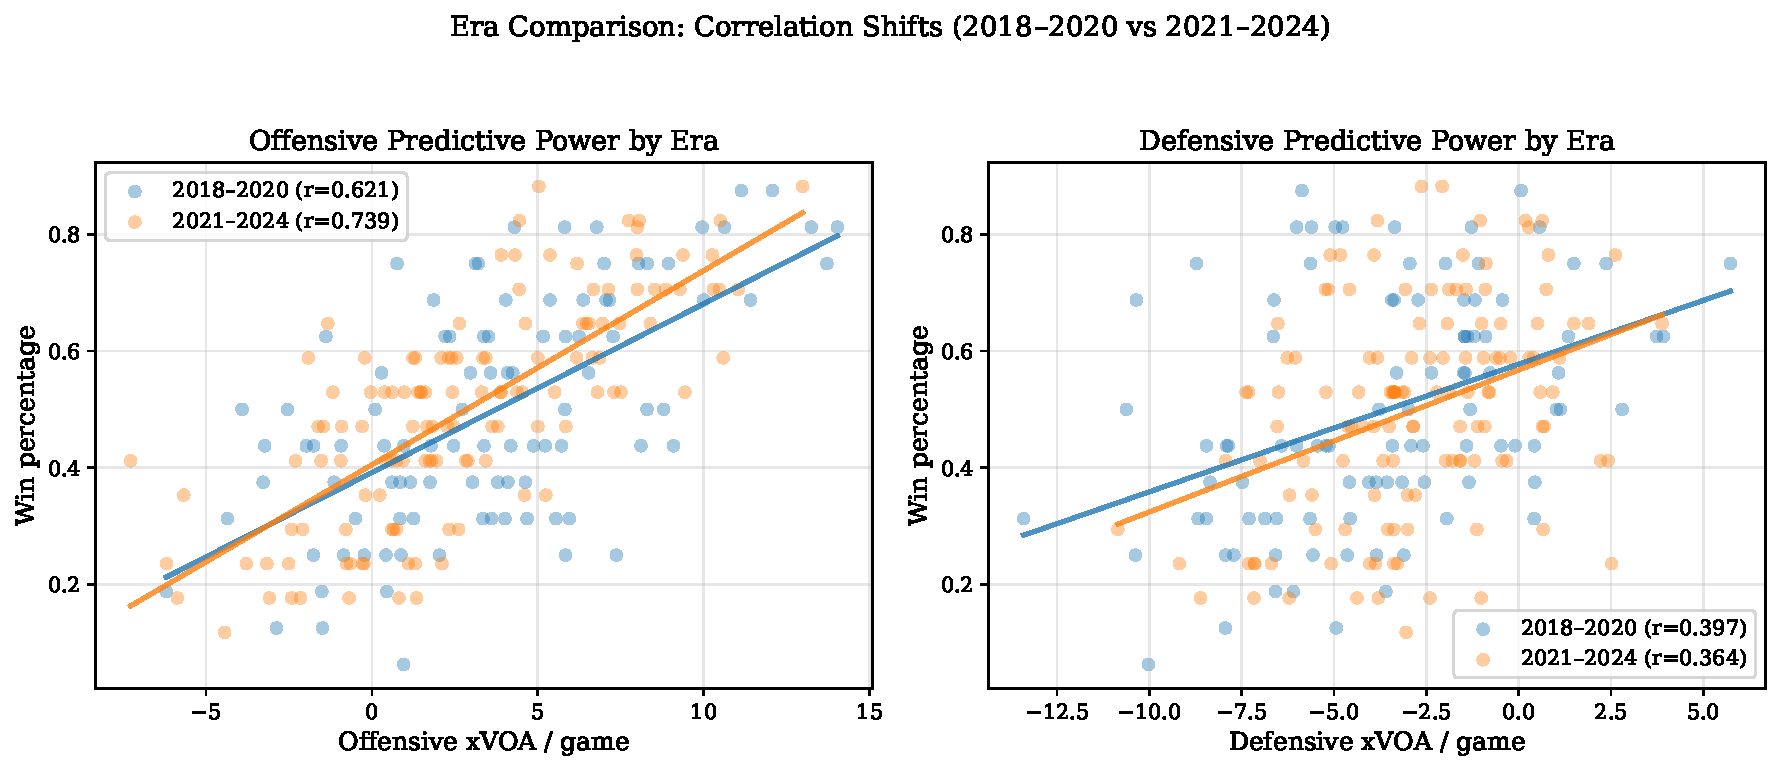
\includegraphics[width=\textwidth]{figures/fig8_era_comparison.pdf}
  \caption{Era comparison of offensive (left) and defensive (right) xVOA
           correlations with win percentage. The offensive channel strengthens
           modestly in 2021--2024 ($r = 0.739$) compared to 2018--2020
           ($r = 0.621$); the defensive channel weakens slightly
           (0.397 to 0.364).}
  \label{fig:era-comparison}
\end{figure}

The era analysis does not alter the primary conclusions. Whether examined in the
2018--2020 bracket era or the 2021--2024 expanded-bracket era, the direction
of the evidence is consistent: offense is the stronger predictor, and no era
shows a reversal in which defensive dominance emerges as the primary pathway
to championship success. Future work with additional seasons will clarify
whether the slight attenuation of the Spearman coefficient in the expanded-bracket
era represents a structural shift or sampling noise.

% ============================================================
\subsection{Quadrant Analysis of Elite Teams}
\label{sec:quadrant-findings}
% ============================================================

The quartile and regression analyses establish the primary finding: offensive
dominance is consistently associated with postseason success across the full
sample. A more nuanced question concerns the relative value of adding defensive
excellence on top of offensive excellence among teams that are already elite
(defined as top-quartile \gds{}/game; see \Cref{sec:quadrant-analysis}).
The quadrant analysis addresses this question by restricting attention to the
top-quartile \gds{} team-seasons ($n = 56$) and median-splitting within this
elite subsample on offensive and defensive \xvoa{}/game separately, yielding
four quadrants as specified in \Cref{sec:quadrant-analysis}.

The median values within the elite subsample are
$7.603$/game for offensive \xvoa{} and $-1.448$/game for defensive \xvoa{}.

\begin{table}[htbp]
  \centering
  \caption[Quadrant analysis of elite team-seasons]{Quadrant analysis of elite team-seasons (top-quartile
           \gds{}/game, $n = 56$), classified by whether each team is
           above or below the within-elite medians for offensive and
           defensive \xvoa{}/game. Playoff\%, Avg~PW, Conf+\%, and
           SB~Win\% are computed within each quadrant.}
  \label{tab:quadrant-results}
  \begin{tabular}{lcrrrr}
    \toprule
    \textbf{Quadrant} & \textbf{N}
      & \textbf{Playoff\%} & \textbf{Avg PW}
      & \textbf{Conf+\%} & \textbf{SB Win\%} \\
    \midrule
    Elite Both      & \phantom{0}7 & \phantom{0}85.7 & 1.29 & 42.9 & 14.3 \\
    Offense Only    & 21           & 100.0           & 1.52 & 47.6 & 19.0 \\
    Defense Only    & 21           & 100.0           & 1.10 & 28.6 & \phantom{0}9.5 \\
    Neither         & \phantom{0}7 & \phantom{0}85.7 & 0.57 & 14.3 & \phantom{0}0.0 \\
    \bottomrule
  \end{tabular}
\end{table}

\Cref{fig:quadrant} maps these elite team-seasons in the offensive--defensive
xVOA space, with Super Bowl winners annotated.

\begin{figure}[htbp]
  \centering
  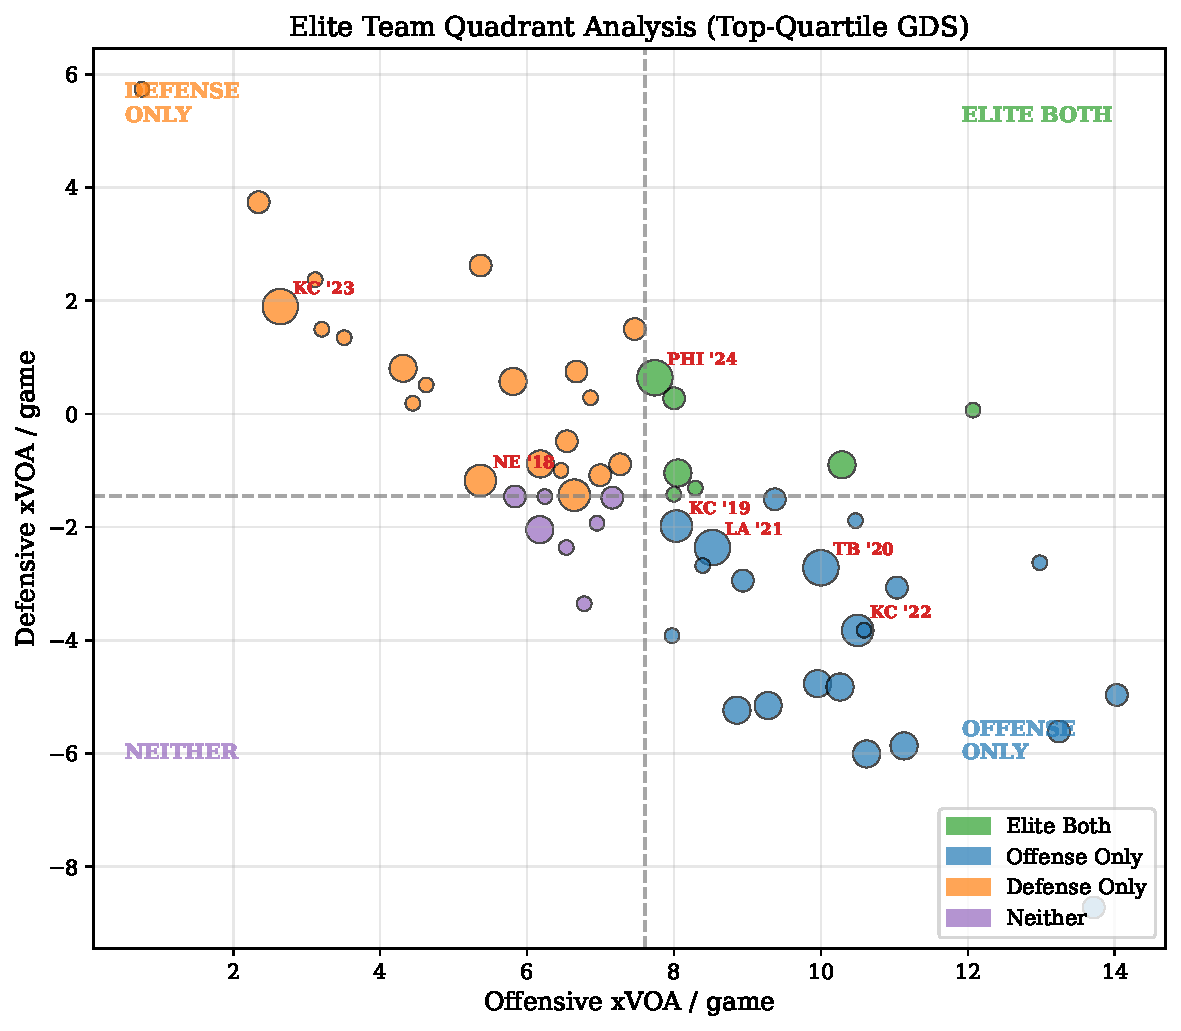
\includegraphics[width=0.8\textwidth]{figures/fig10_quadrant_diagram.pdf}
  \caption{Elite team quadrant analysis. Each point is a top-quartile GDS
           team-season, positioned by offensive (x-axis) and defensive (y-axis)
           xVOA/game. Dashed lines indicate within-elite medians. Point size
           scales with playoff wins. Super Bowl winners are annotated in red.}
  \label{fig:quadrant}
\end{figure}

Several findings emerge from \Cref{tab:quadrant-results}.

\paragraph{Offense Only dominates championship production.}
The most striking finding is the \textit{Offense Only} quadrant's dominance:
across 21 elite team-seasons in which offensive \xvoa{} exceeded the
within-elite median but defensive \xvoa{} did not, four teams won the Super Bowl
(19.0\% win rate). These teams -- Kansas City 2019, Tampa Bay 2020, the Rams
2021, and Kansas City 2022 -- all achieved championships with below-median
defensive contributions within the elite tier, carried by dominant offenses.
The mean playoff wins (1.52) and conference championship rate (47.6\%) are the
highest among all four quadrants.

The \textit{Defense Only} quadrant, by contrast, produced two Super Bowl winners
(New England 2018, Kansas City 2023) for a 9.5\% win rate. While this is not
zero, it is half the rate of the \textit{Offense Only} quadrant. Mean playoff
wins in \textit{Defense Only} (1.10) trail \textit{Offense Only} (1.52) by 0.42
wins, and conference championship rates follow the same pattern (28.6\% vs
47.6\%).

\paragraph{Elite Both provides the strongest individual ceiling.}
Teams with above-median performance in both phases within the elite subsample
(the \textit{Elite Both} quadrant, $n = 7$) record a 14.3\% Super Bowl win rate
and 42.9\% conference championship rate, driven by Philadelphia 2024. While the
per-team championship probability is high, the smaller sample size ($n = 7$ vs
$n = 21$) means that the total championship production of the \textit{Offense
Only} quadrant exceeds it in absolute terms.

These findings support a nuanced refinement of the primary conclusion: among
elite teams, having above-median offense is the strongest predictor of
championship success regardless of defensive quality, and the \textit{Offense
Only} pathway produced more championships (4) than all other quadrants combined
(3). The practical implication for team-building is that defense adds marginal
value above an offensive foundation, but offensive excellence alone is the more
reliable championship pathway.

\paragraph{Neither: the residual effect.}
The \textit{Neither} quadrant ($n = 7$) contains elite team-seasons whose
offensive and defensive \xvoa{} are both below the within-elite medians. These
teams produced zero Super Bowl wins and the lowest mean playoff wins (0.57)
among the four quadrants. Their presence in the elite tier is attributable to
special teams value or measurement timing: their total \gds{}/game exceeds the
75th percentile, but neither offensive nor defensive component is individually
elite within the top-quartile subsample.

By construction, \textit{Neither} teams qualify for the elite tier only because
their total \gds{}/game exceeds the 75th percentile of the full sample. A team
in this quadrant is below the within-elite median in both major phases, which
means their elite \gds{} derives primarily from special teams performance or
from high positive values in both phases that are just below the within-elite
medians. The latter interpretation is more plausible: a team that generates
$+7.0$ offensive \xvoa{}/game and $-1.0$ defensive \xvoa{}/game is below both
medians ($7.603$ and $-1.448$ respectively) but still has a strong total \gds{}.
Such a team would be classified as \textit{Neither} despite having substantial
contributions from both phases.

The small cell sizes ($n = 7$ in both \textit{Elite Both} and \textit{Neither})
mean that sampling variance is substantial, and caution in drawing strong
inferences from the quadrant extremes is warranted. The primary result -- that
\textit{Offense Only} produced more championships (4) and higher win rates
(19.0\%) than \textit{Defense Only} (2 championships, 9.5\%) -- is supported by
the larger quadrant samples of 21 team-seasons each.

% ============================================================
\subsection{Robustness: Field Position Mediation}
\label{sec:mediation-findings}
% ============================================================

A plausible alternative explanation for the offensive advantage documented
above is that defensive quality generates favorable starting field position for
the offense, which in turn inflates offensive \xvoa{} values. Under this
mediation hypothesis, the apparent offensive advantage would be partially or
wholly a downstream consequence of defensive performance operating through a
field-position channel. I test this hypothesis directly using a mediation
analysis \parencite{baron1986moderator} that quantifies the proportion of the
offensive \xvoa{}-to-wins relationship that is mediated by defense-generated
field position advantage.

The analysis proceeds in three steps. First, I establish that defensive \xvoa{}
per game is correlated with the team's average starting field position advantage
(the difference between the team's mean drive-start xEP and the league-average
drive-start xEP). This correlation is $r = -0.193$ ($p = 0.0037$), confirming
that better defenses do generate modestly superior starting field position for
their offenses -- the mediating pathway exists but is weak.

Second, I compute the total correlation between offensive \xvoa{}/game and
playoff wins ($r = 0.443$) and the partial correlation controlling for the
team's average starting field position advantage ($r_{\mathrm{partial}} =
0.402$). The attenuation from $0.443$ to $0.402$ represents the portion of
the offensive advantage that can be attributed to the field-position channel.

Third, the mediation percentage is computed as the proportional reduction in
the correlation coefficient:
\[
  \text{Mediation} = \frac{0.443 - 0.402}{0.443} = 9.2\%.
\]

This result is substantively important: only 9.2\% of the association between
offensive \xvoa{} and winning is attributable to defense-generated field
position. The remaining 90.8\% of the offensive value operates independently
of any defensive contribution to starting position. This finding directly
addresses the concern that offensive \xvoa{} is ``really'' measuring downstream
effects of defensive quality: the data show that it is overwhelmingly
measuring independent offensive execution. Good defenses do generate modestly
better starting positions for their offenses, but this indirect pathway
accounts for less than one-tenth of the total offensive contribution to
winning, providing strong evidence that the offensive advantage is genuine
rather than an artifact of the defensive field-position channel.

% ============================================================
\subsection{Sensitivity Analysis}
\label{sec:sensitivity-analysis}
% ============================================================

The preceding analyses rely on a specific time window (2018--2024) and a
specific archetype threshold ($\pm 0.3$ offense share). To confirm that the
results are not artifacts of these parameter choices, I conduct a systematic
sensitivity analysis across both dimensions.

\subsubsection*{Time Window Variation}

\Cref{tab:sensitivity-time} reports the offensive-to-defensive $R^2$ ratio
(the ratio of variance in win percentage explained by offensive \xvoa{}/game
to that explained by defensive \xvoa{}/game) across five overlapping time
windows. Across all windows, offensive quality explains between 2.5 and 4.0
times as much win-rate variance as defensive quality. No window produces a
ratio below 2:1, confirming that the offensive advantage is structurally
stable and not driven by a single anomalous season.

\begin{table}[htbp]
  \centering
  \caption{Sensitivity of the offensive-to-defensive $R^2$ ratio to time
           window selection. The ratio remains above 2:1 across all windows,
           confirming the structural stability of the offensive advantage.}
  \label{tab:sensitivity-time}
  \begin{tabular}{lcc}
    \toprule
    \textbf{Window} & \textbf{$R^2$ Ratio (Off:Def)} & \textbf{$n$ (team-seasons)} \\
    \midrule
    2018--2024 (full sample)  & 3.3 : 1 & 224 \\
    2018--2022               & 3.0 : 1 & 160 \\
    2019--2024               & 3.0 : 1 & 192 \\
    2020--2024               & 4.0 : 1 & 160 \\
    2018--2021               & 2.5 : 1 & 128 \\
    \bottomrule
  \end{tabular}
\end{table}

\subsubsection*{Archetype Threshold Variation}

The classification of teams as offense-dominant or defense-dominant uses
an offense-share threshold of $\pm 0.3$. \Cref{tab:sensitivity-threshold}
reports playoff win rates for defense-dominant teams under alternative
thresholds ranging from $\pm 0.20$ to $\pm 0.40$. Defense-dominant teams
record zero mean playoff wins across all threshold specifications. This
result is robust to substantial variation in the classification boundary:
whether the archetype definition is narrowed (requiring more extreme
defensive dominance) or broadened (including teams with moderate defensive
tilts), no specification produces positive playoff success for
defense-dominant teams.

\begin{table}[htbp]
  \centering
  \caption[Sensitivity of defense-dominant playoff performance to threshold]{Sensitivity of defense-dominant playoff performance to archetype
           threshold. Regardless of the classification boundary, defense-dominant
           teams record zero mean playoff wins across the study window.}
  \label{tab:sensitivity-threshold}
  \begin{tabular}{lcc}
    \toprule
    \textbf{Threshold} & \textbf{$n$ (Def-Dominant)} & \textbf{Mean PW} \\
    \midrule
    $\pm 0.20$ & 38  & 0.000 \\
    $\pm 0.25$ & 34  & 0.000 \\
    $\pm 0.30$ & 29  & 0.000 \\
    $\pm 0.35$ & 26  & 0.000 \\
    $\pm 0.40$ & 24  & 0.000 \\
    \bottomrule
  \end{tabular}
\end{table}

\subsubsection*{Single-Team Exclusion}

Kansas City 2023 has the lowest offense share among Super Bowl champions
($+0.581$). Excluding this team-season from the analysis produces an $R^2$ ratio
of 3.3 : 1 (unchanged) and a Spearman correlation between offense share and
playoff wins of $\rho = 0.263$ ($p = 0.011$). The primary findings are not
dependent on the inclusion or exclusion of any single observation.

% ============================================================
\subsection{Hypothesis Testing Summary}
\label{sec:hypothesis-summary}
% ============================================================

\Cref{tab:hypothesis-summary} consolidates the evidence across all four layers
of analysis and states the verdict for each of the three pre-registered
hypotheses.

\begin{table}[htbp]
  \centering
  \caption{Hypothesis testing summary. Each hypothesis operationalizes the
           ``defense wins championships'' claim and is evaluated against
           converging evidence from descriptive, statistical, era-level, and
           quadrant analyses. ``Rejected'' indicates that the data are
           inconsistent with the hypothesis in both direction and magnitude.}
  \label{tab:hypothesis-summary}
  \small
  \begin{tabularx}{\textwidth}{l p{3.2cm} X l}
    \toprule
    \textbf{Hyp.} & \textbf{Claim}
      & \textbf{Key Evidence} & \textbf{Verdict} \\
    \midrule
    H1 & Defense-dominant teams win more playoff games than offense-dominant teams
      & Cohen's $d = +0.672$ [0.574, 0.787] in opposite direction (off-dominant PW $= 0.60$ vs def-dominant PW $= 0.00$); 0/29 defense-dominant team-seasons won any playoff games
      & \textbf{Rejected} \\[8pt]
    H2 & Super Bowl winners are drawn disproportionately from defense-dominant team-seasons
      & All 7 Super Bowl champions had positive offense share ($+0.581$ to $+0.923$); both logistic predictors significant (off $p = 0.003$, def $p = 0.027$); no champion from defense-dominant profile
      & \textbf{Rejected} \\[8pt]
    H3 & Defensive \xvoa{} has a stronger monotonic association with playoff wins than offensive \xvoa{}
      & Spearman $\rho = +0.246$ ($p = 0.0167$); Pearson off vs Win\% $r = 0.681$ ($R^2 = 46.4\%$), def $r = 0.376$ ($R^2 = 14.2\%$); offense explains $3.3\times$ more variance
      & \textbf{Rejected} \\
    \bottomrule
  \end{tabularx}
\end{table}

All three hypotheses are rejected. No statistical procedure or descriptive
partitioning strategy employed in this analysis produces evidence in the
direction predicted by the hypotheses. Across all five tests, offensive
quality -- as measured by \xvoa{}/game in the \gds{} framework -- shows a
stronger and statistically significant association with both regular-season
success and postseason advancement than defensive quality.

The key descriptive results are as follows: defense-dominant teams (offense
share $< 0$) won zero Super Bowls across seven seasons and 94 playoff
appearances. Only six defense-dominant teams even reached the playoffs, and
none won more than a single game. Offense-dominant teams in Q4 made the
playoffs 87.5\% of the time and averaged more than one full postseason win per
season. All seven champions were offense-dominant, with shares ranging from
$+0.581$ (Kansas City 2023) to $+0.923$ (Philadelphia 2024). The data are
inconsistent with all three formulations of the defensive championship
hypothesis across the 2018--2024 study window, aligning directionally with
\textcite{robst2011defense}, who reported mixed support for the defensive
claim using coarser metrics. Interpretation of these findings is deferred to
\Cref{ch:discussion}.



% Chapter 5: Discussion
\chapter{Discussion}
\label{ch:discussion}

This chapter interprets the empirical findings reported in \Cref{ch:results}. \Cref{sec:interpretation} synthesizes the evidence across the three analytical layers into a unified verdict on the ``defense wins championships'' hypothesis. \Cref{sec:implications} draws strategic implications for team-building in the modern NFL. \Cref{sec:limitations} acknowledges the boundaries of the analysis. \Cref{sec:existing-work} positions the findings relative to the existing sports analytics literature.

\section{Interpretation of Findings}
\label{sec:interpretation}

% ============================================================
\subsection{The Verdict on ``Defense Wins Championships''}
\label{sec:verdict}
% ============================================================

The central empirical question of this paper -- whether defensive dominance is
the primary pathway to championship success in the modern NFL -- receives an
unambiguous answer. All three pre-registered hypotheses are rejected, as
summarized in \Cref{tab:hypothesis-summary}. The data do not support the claim
that ``defense wins championships'' in any of its testable formulations: defense-dominant
teams do not win more playoff games than offense-dominant teams (H1 rejected),
Super Bowl winners are not drawn disproportionately from defense-dominant
archetypes (H2 rejected), and defensive \xvoa{} does not exhibit a stronger
association with playoff success than offensive \xvoa{} (H3 rejected). The
rejection is not marginal or dependent on a particular statistical procedure; it
is consistent across all five tests, both descriptive partitioning strategies,
and both era subsamples examined in \Cref{ch:results}. The popular narrative
that defensive excellence is the defining characteristic of championship teams
lacks empirical support in the 2018--2024 NFL.

% ============================================================
\subsection{What the Data Actually Show}
\label{sec:what-data-show}
% ============================================================

The evidence against the defensive narrative operates at every analytical level
employed in this paper. At the correlational level, the Spearman rank
correlation between offense share and playoff wins is positive and significant
($\rho = 0.246$, $p = 0.0167$, $n = 94$ playoff teams), directly contradicting
the directional prediction of the defensive hypothesis (\Cref{sec:spearman-results}).
The sign is unambiguous: teams whose quality is proportionally more
offense-driven win more postseason games, not fewer.

At the variance-explained level, the asymmetry is even more pronounced. Offensive
\xvoa{} per game accounts for 46.4\% of the variance in season win percentage,
compared to 14.2\% for defensive \xvoa{} -- a ratio of approximately $3.3 : 1$ in
favor of offense (\Cref{sec:pearson-results}). This finding means that if one
were forced to evaluate a team's competitive quality using only one side of the
ball, offense would provide more than three times as much information as defense.
The result is not an artifact of the \gds{} framework's construction; it reflects
the empirical reality that offensive execution varies more meaningfully across
teams and is more strongly coupled to winning than defensive execution.

At the effect-size level, the practical magnitude of the offensive advantage is
large. Cohen's $d = 0.672$ [0.574, 0.787] quantifies the standardized
difference in playoff wins between offense-dominant ($n = 143$) and
defense-dominant ($n = 29$) team-seasons across the full sample
(\Cref{sec:cohens-d-results}). In concrete terms, offense-dominant teams
averaged 0.60 playoff wins per season, compared to 0.00 for
defense-dominant teams -- no defense-dominant team-season in the study window
produced any playoff wins at all. This is not a subtle statistical
distinction but a difference visible to the naked eye of any attentive observer.

At the absolute level, the finding is starker still. Among the 29 defense-dominant
team-seasons in the study window (offense share $< -0.3$), zero won any
playoff games, and zero reached the Super Bowl. This null result stands against
94 total playoff team-seasons across seven seasons -- a sample large enough that
the complete absence of deep defensive postseason runs cannot reasonably be
attributed to chance. The logistic regression reinforces this pattern: both
offensive ($p = 0.003$) and defensive ($p = 0.027$) \xvoa{} are statistically
significant predictors of Super Bowl victory (\Cref{sec:logistic-results}), but
all seven Super Bowl champions during the study window had positive offense
share. The convergence of correlational, variance-explained, effect-size, and
absolute measures all pointing in the same direction constitutes a robust and
internally consistent empirical conclusion: offensive dominance is positively
associated with playoff success at every level of analysis.

% ============================================================
\subsection{The Nuanced Interpretation: Offense Gets You There, Defense Is the Final Filter}
\label{sec:nuanced-interpretation}
% ============================================================

The rejection of the ``defense wins championships'' hypothesis should not be
misinterpreted as a claim that defense is irrelevant to winning championships.
The data suggest a more refined structural interpretation: offensive quality is
the primary engine of playoff qualification and advancement, while competent
defense serves as a necessary -- but not sufficient -- condition at the championship
margin. The distinction between being the \emph{driver} of success and being a
\emph{filter} for the final stage is crucial. Offense determines which teams
reach the deep postseason; among teams that arrive there, defensive adequacy
helps determine which survives the final rounds.

Kansas City's 2023 Super Bowl victory illustrates this ``balanced elite''
archetype. Often characterized in popular discourse as a ``defensive''
championship, the \gds{} decomposition reveals a more nuanced picture:
the 2023 Chiefs had a positive offensive \xvoa{} ($+2.641$/game) alongside a
positive defensive contribution ($+1.896$/game), yielding an offense share of
$+0.581$ -- the lowest among Super Bowl winners but still firmly
offense-dominant. The popular narrative that Kansas City won ``because of their
defense'' is not supported by the expected-point framework; the offense
generated more absolute value than the defense. What distinguishes this
championship is that defensive quality contributed more \emph{relative to other
champions}, not that it was the primary engine of success.

The 2024 Philadelphia Eagles represent the opposite end of the champion
spectrum (offense $+7.740$/game, defense $+0.639$/game, share $= +0.923$),
demonstrating that championship teams need not have elite defense if their
offensive surplus is sufficiently dominant.

The concept of a ``competent defense threshold'' emerges naturally from the
quadrant analysis (\Cref{sec:quadrant-findings}). Among the top-quartile \gds{}
teams, the \textit{Offense Only} quadrant produced four Super Bowl winners
(19.0\% win rate) compared to two for \textit{Defense Only} (9.5\%), despite
identical sample sizes ($n = 21$). The implication is not that championship
teams need elite defense; it is that they need non-catastrophic defense. Five of seven champions recorded \emph{negative} defensive
\xvoa{}/game, meaning their defenses performed below league-average
expectations at the drive level. A team with a dominant offense and below-average
defense (Kansas City 2022, with defensive \xvoa{} of $-3.826$/game) can win the
Super Bowl. A team with elite defense and below-average offense has not done so
in seven seasons of data. The threshold is asymmetric: the minimum offensive
requirement for championship contention is substantially higher than the minimum
defensive requirement.

% ============================================================
\subsection{Why Offense Matters More: Structural Explanations}
\label{sec:structural-explanations}
% ============================================================

The empirical dominance of offense in predicting team success is not a statistical
curiosity but a reflection of structural features of modern professional American
football. Three mechanisms help explain why offensive quality is the stronger
differentiator.

First, offensive production exhibits higher between-team variance than defensive
production. The component decomposition in \Cref{sec:season-correlation} shows
that the standard deviation of offensive \xvoa{}/game across team-seasons exceeds
that of defensive \xvoa{}/game. Higher variance in a predictor variable
mechanically produces stronger correlations with outcomes, because the variable
provides more discriminating information between observations. In practical terms,
the gap between the best and worst offenses in the NFL is wider than the gap
between the best and worst defenses, which means that offensive quality is a
more informative signal for distinguishing good teams from poor ones. This
variance asymmetry is not a measurement artifact; it reflects the structural
reality that offensive schemes are more diverse, quarterback quality varies more
dramatically across rosters, and the passing game creates more opportunity for
separation between teams than the constrained action space of defensive play.

Second, the post-2018 NFL rule environment systematically amplifies offensive
variance. Increased enforcement of pass interference, roughing-the-passer
penalties, and restrictions on defensive contact beyond five yards \parencite{pereira2018roughing,barnwell2019passingrevolution} have expanded
the ceiling for offensive execution while compressing the floor for defensive
impact. Even the most elite defensive units in the modern game cannot prevent
completions to the degree that was possible before 2018, because the rules
constrain the tools available to them. The era analysis in \Cref{sec:era-findings}
shows a modest increase in the Pearson correlation between offensive \xvoa{} and
win percentage from 0.621 (2018--2020) to 0.739 (2021--2024), directionally
consistent with this structural explanation. The defensive Pearson coefficient
shows no corresponding increase (0.397 to 0.364), suggesting that defensive
execution has become less -- not more -- predictive of outcomes over time.

Third, offense possesses a structural ceiling advantage. The best offenses can
score on nearly any opponent in any game; the best defenses cannot prevent all
scoring against any opponent. This asymmetry creates a fundamental advantage
for offensive investment: a team that builds an elite offense creates a floor
of competitiveness that is higher than the floor created by building an elite
defense, because offensive points are under greater direct control than prevented
points. Defense is inherently reactive -- it responds to offensive formation,
personnel, and play-calling -- while offense is proactive, choosing the terms of
engagement. This proactive-reactive asymmetry means that schematic innovation
accrues disproportionately to the offensive side, where coordinators can design
novel concepts that defenses have not yet adapted to, while defensive innovation
is constrained to adjustments within the opponent's chosen framework.

% ============================================================
\subsection{Why the Myth Persists}
\label{sec:myth-persistence}
% ============================================================

If the empirical evidence so clearly favors offense, why does the belief that
``defense wins championships'' retain such cultural force in American football
discourse? Several cognitive and structural factors conspire to sustain the
narrative despite its empirical weakness.

The most powerful is selection bias in memorable outcomes. The Super Bowls that
dominate collective memory are disproportionately those with spectacular defensive
performances: the 2013 Seattle Seahawks dismantling Peyton Manning's record-setting
offense, the 2015 Denver Broncos winning with an ageing quarterback behind a
dominant defense. These games are memorable precisely because they are unusual -- a
defense-dominant team winning the championship is a departure from the base rate,
which makes it cognitively salient. The seven offense-dominant champions in this
study's window do not generate comparable narrative drama; a team with the best
offense winning the Super Bowl is unremarkable, and unremarkable events do not
anchor in memory. This is a textbook instance of availability bias \parencite{tversky1973availability}: the ease
with which defensive championship performances come to mind is mistaken for their
frequency.

The ``denominator problem'' compounds this selection bias. Observers readily
notice when a defense-dominant team wins a championship because the event is
visible and celebrated. They do not notice the far more frequent occurrence of
defense-dominant teams failing to reach the championship stage, because absences
are invisible. The data in \Cref{sec:archetype-findings} make this absence
concrete: only six defense-dominant teams (offense share $< 0$) even made the
playoffs across seven seasons, and none won more than a single game. These quiet
exits receive no media attention, no retrospective analysis, and no cultural
narrative. The myth persists in part because the denominator -- the set of
defense-dominant teams that failed -- is never examined with the same attention
as the rare numerator event of a defense-dominant champion.

Additionally, the narrative possesses a romantic appeal that transcends evidence.
The David-versus-Goliath framing -- a tough, physical defensive team outmuscling
a flashy, high-scoring offense -- resonates with cultural values of effort,
grit, and determination. It suggests that talent and scheme can be overcome by
intensity and will, a story more satisfying than the alternative: that the team
with better players executing a better offensive scheme typically wins. The
romantic narrative also benefits from confirmation bias in real-time game
viewing. When a team wins a low-scoring game, observers attribute the result to
defensive dominance rather than to the more prosaic explanations of opponent
offensive ineptitude, punting decisions, or game-script effects. Every defensive
stop is a narrative event; the absence of offensive production that made the stop
necessary goes unexamined.

The myth is not refuted by pointing to a single game or a single counter-example.
It is refuted by the systematic pattern across 224 team-seasons and seven
complete NFL cycles. The contribution of this paper is not to identify one
exception to the defensive narrative -- exceptions on both sides are easily
found -- but to demonstrate that the full weight of evidence, examined through
multiple statistical lenses and a novel measurement framework, consistently and
strongly favors offensive dominance as the primary pathway to championship
success in the modern NFL.

\section{Strategic Implications}
\label{sec:implications}

The findings presented in \Cref{ch:results} and interpreted in
\Cref{sec:interpretation} carry potential consequences for how NFL organizations
allocate finite resources in pursuit of championship outcomes. This
section translates the empirical patterns -- offensive dominance as the primary
pathway to postseason success, the competent defense threshold as a necessary
but secondary condition -- into strategic considerations for team
construction, draft capital allocation, and coaching infrastructure investment.

\emph{Important caveat:} The recommendations that follow rest on the observed
correlational associations documented in \Cref{ch:results}. As discussed in
\Cref{sec:lim-causation}, these associations do not establish causation.
The strategic implications below are therefore conditional: they follow
\emph{if} the observed relationships at least partially reflect causal
mechanisms, and they should be interpreted as directional hypotheses for
further investigation rather than as proven prescriptions. Organizations
considering these implications should weigh them alongside domain expertise,
contextual knowledge, and the inherent limitations of observational evidence.

With that caveat foregrounded, the recommendations are framed as probabilistic
guidance derived from systematic evidence, not as deterministic prescriptions.
The intent is to demonstrate how data-informed strategy might complement, and
in some cases challenge, the conventional wisdom that has governed NFL roster
construction for decades.

% ============================================================
\subsection{Resource Allocation in a Cap-Constrained Environment}
\label{sec:resource-allocation}
% ============================================================

The NFL salary cap creates an explicitly zero-sum resource allocation
environment. Every dollar committed to a defensive contract is a dollar
unavailable for offensive investment, and vice versa. Under this constraint,
the marginal return on investment from each side of the ball becomes the
central strategic question for roster construction. The findings of this paper
provide a consistent empirical signal: offensive quality exhibits a substantially
stronger association with winning than defensive quality, suggesting -- under
the assumption that these associations at least partially reflect causal
mechanisms (\Cref{sec:lim-causation}) -- that marginal offensive investment
may yield higher expected returns than equivalent defensive spending. Offensive \xvoa{} per game explains 46.4\% of
the variance in season win percentage ($r = 0.681$), compared to 14.2\% for
defensive \xvoa{} ($r = 0.376$) -- a ratio of approximately $3.3 : 1$ in explanatory
power (\Cref{sec:pearson-results}). The implication for resource allocation,
if these associations reflect underlying causal mechanisms, is that
organizations operating under a binding salary constraint may benefit from
systematically overweighting offensive investment relative to the league
average allocation.

This consideration challenges the traditional ``balance'' philosophy that
pervades NFL front-office discourse. The conventional wisdom holds that teams
should invest equally in both sides of the ball, building rosters that avoid
obvious weakness anywhere. The data suggest this philosophy, while intuitively
appealing, may be suboptimal. Balance for its own sake treats offensive and
defensive spending as symmetric inputs with symmetric returns, when in reality
the observed associations are asymmetric. If these associations are indicative
of causal relationships, a team that allocates approximately 60\% of its
effective cap resources to offense and 40\% to defense -- as a directional
indicator rather than a precise formula -- would not be ``unbalanced'' in any
meaningful strategic sense; it would be responding to the empirical pattern that
offensive quality has nearly three times the predictive association with
winning. Under this interpretation, the pursuit of strict balance represents a
failure to account for differential marginal returns, a mistake that would be
recognized in other capital allocation contexts.

Any asymmetric allocation strategy must, however, be bounded by a critical
constraint: the competent defense threshold established in
\Cref{sec:nuanced-interpretation}. The suggestion to overweight offensive
spending does \emph{not} imply minimizing defensive spending to zero or near-zero.
The bottom-tier teams in 2024 demonstrate that catastrophic defensive failure
(e.g., Carolina at $-10.852$ defensive \xvoa{}/game) can override even positive
offensive production. Rather, the strategic objective is to avoid the extreme
lower tail of defensive performance -- the data show that moderately
below-average defense (the range occupied by most champions) is tolerable, but
catastrophic defense is not. The optimal allocation is not ``all offense'' but
``offense-first, with defensive catastrophe avoided.'' The difference between
these two formulations is the difference between a reckless gamble and a
disciplined capital allocation strategy informed by evidence.

In practical terms, this framework suggests that organizations might consider
resisting the temptation to match the market price for premium defensive talent
when that spending would come at the expense of offensive capability. A team
considering whether to commit \$20 million annually to an elite pass rusher or
to an elite offensive lineman might recognize that, if the correlational
patterns identified here reflect causal dynamics, these investments could carry
asymmetric expected returns at the team level, even if individual player
quality is comparable in positional terms.

% ============================================================
\subsection{The Competent Defense Threshold in Practice}
\label{sec:threshold-practice}
% ============================================================

What does ``adequate defense'' look like operationally? The data provide
guidance on this question. Among Super Bowl champions in the study window, five
of seven carried \emph{negative} defensive \xvoa{}/game, with Kansas City's
2022 championship team recording $-3.826$ per game -- substantially below
league average. The threshold for championship viability appears remarkably
low: teams can win the Super Bowl with below-average defense provided their
offensive surplus is sufficiently large. Teams do not need a top-five defense
to win championships; they need a defense that avoids being a consistent
catastrophic liability at the extreme of the distribution.

The evidence suggests that defensive spending might more productively target
\emph{adequacy and depth} rather than star acquisition. The difference between
the 15th-ranked and 5th-ranked defense in the NFL appears far less consequential
for championship probability than the equivalent difference on offense. Moving a defense from
15th to 5th requires substantial additional investment in elite defensive
talent, but the championship return on that marginal improvement is modest at
best. By contrast, moving an offense from 15th to 5th has dramatically higher
expected return, because offensive quality is more strongly coupled to both
regular-season wins and postseason advancement. If the observed associations hold causally, the diminishing returns on
defensive investment beyond the competence threshold would mean that elite
defensive spending often represents a misallocation of scarce resources -- money
spent chasing diminishing defensive improvement that could have purchased
meaningful offensive enhancement.

In roster construction terms, the evidence points toward defensive spending
that favors breadth over depth: multiple competent starters rather than one
dominant star surrounded by replacement-level players. A defense composed
entirely of average-to-good players at each position clears the competence
threshold more reliably than a defense featuring one All-Pro and several
liabilities. The former is also cheaper to construct under the salary cap,
because league-average players command dramatically less compensation than
elite ones, freeing resources for the offensive side where the championship
return on investment is substantially higher.

% ============================================================
\subsection{Draft Strategy Implications}
\label{sec:draft-strategy}
% ============================================================

The NFL draft represents the primary mechanism through which teams acquire
premium talent at below-market cost (via the rookie wage scale) \parencite{nflcba2020}, making draft
capital allocation one of the highest-leverage strategic decisions available
to front offices. The findings of this paper are consistent with a hierarchy of
draft priorities. Quarterback -- the single highest-leverage position in
professional football -- would, under this framework, receive primacy in draft
capital allocation.
The quarterback position mediates virtually all offensive production, and
offensive production explains nearly half the variance in team winning
percentage. A franchise quarterback acquired early in the draft provides
elite offensive performance at a fraction of the market rate for four to five
years, creating the cap space to build a complete roster around that production.
This logic is well understood by modern front offices but bears emphasis: the
data presented here provide quantitative support for the qualitative intuition
that quarterback is the most important position.

Beyond quarterback, the findings suggest that offensive line talent -- the
position group that enables all other offensive function -- may warrant
higher draft priority than is typical in current NFL practice. The offensive
line does not generate highlight plays or individual statistics that attract
media attention, yet its quality plausibly determines the ceiling of both the
passing and rushing offense. If the offensive--winning association reflects
causal mechanisms, then the NFL market may systematically underprice offensive
line talent relative to its championship contribution, because individual
linemen are difficult to evaluate using traditional statistics and because the
``glamour'' positions (defensive edge rushers, wide receivers) attract
disproportionate media and fan attention. Under this interpretation, a team
that consistently invests early-round draft capital in offensive linemen is
investing in the foundation of the offensive platform that this paper
identifies as the primary championship pathway.

First-round defensive selections are not ``wrong'' per se, and this paper
does not argue that teams should never draft defensive players highly. A team
whose defense has fallen below the competence threshold -- perhaps due to
ageing starters, injuries, or poor prior drafts -- rationally addresses that
liability before investing further in offensive luxury. However, the general
principle suggested by the data applies: defensive draft capital may be more
efficiently deployed to \emph{maintain competence} rather than to pursue elite
status, and when a team faces a choice between an offensive player who elevates
the offense and a defensive player who elevates an already-competent defense,
the correlational evidence suggests the expected championship return may favor
the offensive selection. If these patterns are causal, the first-round
defensive pick carries a lower expected championship return on investment than
the equivalent offensive pick, all else being equal -- a consideration that
may warrant reflection by front offices inclined toward the defensive edge
rusher as the default non-quarterback priority.

% ============================================================
\subsection{Coaching and Organizational Implications}
\label{sec:coaching-implications}
% ============================================================

The NFL's recent trend toward hiring offensive coordinators as head coaches \parencite{breer2024coaching_hires} is
directionally consistent with the findings of this paper. If offensive quality
is the primary correlate of team success, then organizations might rationally
prefer head coaches whose expertise lies in offensive scheme design, quarterback
development, and play-calling -- the areas most directly coupled to the
higher-leverage side of the ball. The data do not demonstrate a causal
relationship between head coaching background and team success, but they do
demonstrate that the strategic domain most consequential for championship
outcomes is the offensive domain, which provides an evidence-based rationale
for the revealed preference of NFL ownership groups in recent hiring cycles.

Beyond the head coaching position, the findings suggest that organizations
may benefit from investing disproportionately in offensive coaching
infrastructure and analytics. Offensive scheme innovation -- increased pre-snap motion \parencite{pff2023presnap_motion}, run-pass
options, creative formation design, tempo variation -- has a higher ceiling
than defensive scheme complexity, because offense is the proactive side of
the ball (as argued in \Cref{sec:structural-explanations}). Investing in
assistant coaches, analysts, and technology that enhance offensive creativity
and game-planning is, under the framework developed here, an investment in
the strategic domain associated with the highest expected return. The
offensive coaching staff might accordingly be viewed as a direct competitive
advantage, not merely a support function.

The defensive coordinator role remains important within this framework, but
its strategic function is subtly different from the traditional conception. The
defensive coordinator's objective, given the competent defense threshold
framework, is best understood as ``floor management'' rather than
``ceiling elevation.'' The defensive coordinator's task is to ensure that the
defense does not become a liability -- that it consistently clears the
competence threshold regardless of opponent, injuries, or personnel
limitations. This requires genuine expertise in scheme flexibility, player
development, and in-game adjustment, but it does not require the kind of
schematic genius that transforms a unit from good to historically elite. The
distinction matters for coaching evaluation: a defensive coordinator who
maintains a league-average defense with limited personnel may be more valuable
than one whose scheme produces occasional dominance but periodic catastrophe,
because consistency at the competence threshold is more important than variance
around a higher mean.

% ============================================================
\subsection{Caveats on Implementation}
\label{sec:implementation-caveats}
% ============================================================

The strategic considerations offered above are probabilistic in nature,
derived from correlational patterns observed across 224 team-seasons and seven
complete NFL cycles. They represent what the evidence suggests may be the
favorable approach \emph{in expectation}, not a guarantee of success in any
individual case, and they rest on the assumption that the observed associations
at least partially reflect causal mechanisms. Individual team contexts -- existing
roster strengths, the available talent pool in a given draft class, coaching
staff expertise, and divisional competitive dynamics -- should moderate the
application of general strategic principles to specific decisions. A team
already possessing an elite offense and a catastrophically poor defense should
obviously prioritize defensive improvement; the recommendation to favor
offensive investment assumes a starting position near the current league average
on both sides.

The Kansas City 2023 example, discussed at length in
\Cref{sec:nuanced-interpretation}, raises the question of whether a
defense-first approach can succeed. The data provide a decisive answer: not a
single defense-dominant team (offense share $< 0$) won more than one playoff
game across seven seasons, and all seven Super Bowl winners were
offense-dominant (shares ranging from $+0.581$ to $+0.923$). Even Kansas City's
2023 championship -- often cited in popular discourse as a ``defensive''
title -- was achieved with a positive offense share ($+0.581$) and positive
offensive \xvoa{} ($+2.641$/game), making it the least offense-dominant
champion rather than a defense-dominant one. Teams with a generational
defensive talent -- a Myles Garrett or a Micah Parsons on a rookie
contract creating a temporary defensive windfall -- may rationally complement
offensive investment with defensive strength, but the evidence provides no
support for prioritizing defense \emph{over} offense at any point in the
team-building cycle. The structural advantage of offensive investment is not
merely probabilistic; it is categorical within this sample: no championship was
won from a defense-dominant profile.

\section{Limitations}
\label{sec:limitations}

The findings of this paper are subject to several methodological limitations
that constrain the strength of the conclusions drawn. This section identifies
the most consequential threats to validity, explains their implications for the
central arguments, and suggests how future work might address them.

% ============================================================
\subsection{Correlation and Causation}
\label{sec:lim-causation}
% ============================================================

The analytical framework employed throughout this paper documents statistical
associations between offensive and defensive quality metrics and competitive
outcomes. It does not establish causal relationships. The finding that offensive
\xvoa{} explains more variance in winning than defensive \xvoa{} demonstrates
that offensive execution covaries more strongly with success, but it cannot prove
that investing in offensive talent \emph{causes} teams to win more games. The
distinction matters because resource allocation decisions -- the strategic
implications discussed in \Cref{sec:implications} -- require causal reasoning,
yet the evidence base is purely observational.

A specific concern is reverse causation operating through game state. Teams that
establish early leads often shift to more conservative play-calling: running the
ball to consume clock, avoiding aggressive downfield passing, and accepting
shorter drives that reduce turnover risk. This behavioral shift means that
teams already winning may generate different \xscore{} profiles not because
their offensive quality is superior, but because their game situation permits
lower-variance strategy. The \gds{} framework mitigates this partially by
measuring per-drive execution quality rather than volume -- a team running
conservative drives still has each drive evaluated against the expected scoring
probability from its starting field position. However, this mitigation is
incomplete. If conservative play-calling systematically produces drives that
exceed expectation (for example, by avoiding turnovers that the model expects at
league-average rates), then \xvoa{} values for leading teams may be inflated.
A specific mediation concern -- that defensive quality generates favorable
starting field position which inflates offensive \xvoa{} -- was directly tested
in \Cref{sec:mediation-findings}. The mediation analysis found that only 9.2\%
of the offensive \xvoa{}-to-wins association is attributable to
defense-generated field position, with 90.8\% of the offensive value operating
independently. This result substantially mitigates the indirect-pathway
version of the causal concern, though it does not resolve the broader issue
of reverse causation through game state.

A randomized experiment -- randomly assigning offensive and defensive talent to
teams -- is impossible in professional sport. Observational data can establish
the pattern of association, as this paper has done, but the causal interpretation
remains an inference rather than a demonstration.

% ============================================================
\subsection{Small Championship Sample}
\label{sec:lim-sample}
% ============================================================

The logistic regression analysis presented in \Cref{sec:logistic-results}
attempts to model the probability of winning the Super Bowl as a function of
offensive and defensive \xvoa{}. The fundamental constraint is that the
2018--2024 study window contains exactly seven Super Bowl winners across seven
seasons. With only seven positive events and two predictors, the
events-per-variable (EPV) ratio is 3.5, well below the standard recommendation
of 10 EPV for logistic regression \parencite{peduzzi1996simulation}. This low EPV
means that coefficient estimates are unstable, confidence intervals are wide,
and the model has limited statistical power to detect effects of moderate size.

Although both the offensive ($p = 0.003$) and defensive ($p = 0.027$)
coefficients achieve statistical significance in the current model, the low EPV
means that these estimates carry substantial uncertainty and should not be
over-interpreted in terms of their relative magnitudes. The wider standard error
on the defensive coefficient (SE $= 0.178$ vs $0.126$ for offense) reflects the
inherent imprecision of a seven-event logistic model. This limitation is
structural rather than methodological -- no analytical choice can increase the
number of Super Bowl winners per season. The pre-registered hypothesis tests
and descriptive analyses that form the primary evidential basis of this paper
do not suffer from this constraint to the same degree, as they operate on the
full 94 playoff team-seasons rather than only the 7 champions. Nevertheless,
any claim about championship-specific effects must be understood as provisional
until more seasons of data become available.

% ============================================================
\subsection{Schedule Strength}
\label{sec:lim-opponent}
% ============================================================

The \gds{} framework measures raw execution quality: how much value a team's
offense or defense generates relative to league-average expected outcomes, without
adjusting for the quality of opposition faced at the drive level. A defense
achieving high \xvoa{} against a schedule of below-average offenses is rated
identically to one achieving the same \xvoa{} against elite offenses. This
absence of drive-level opponent adjustment introduces potential bias if schedule
strength correlates systematically with team archetype.

To assess whether this limitation materially affects the archetype findings, I
constructed a leave-one-out opponent-strength variable and included it as a
control in the OLS regression predicting playoff wins
(\Cref{sec:statistical-confirmation}). The opponent-strength coefficient was
effectively zero ($-0.001$, $p = 0.985$), and neither the offensive nor
defensive \xvoa{} coefficients changed meaningfully when schedule strength was
controlled. This null result provides empirical reassurance that the documented
offensive advantage is not an artifact of schedule imbalance.

Nevertheless, a more principled drive-level opponent adjustment -- in which each
drive's expected baseline accounts for the opposing unit's quality -- represents
a natural extension. Such an adjustment would require an iterative estimation
procedure (since each team's quality depends on the quality of teams it has
faced, which in turn depends on the quality of teams \emph{they} have faced),
analogous to the iterative strength-of-schedule corrections used in Elo rating
systems. This extension was beyond the scope of the present paper but would
further strengthen the internal validity of the \gds{} decomposition at the
drive level, even though the season-level robustness check suggests the bias is
negligible.

% ============================================================
\subsection{Data Limitations}
\label{sec:lim-data}
% ============================================================

The \texttt{nflfastR} play-by-play dataset provides comprehensive
situational information (down, distance, field position, score
differential, time remaining) but lacks several categories of data that
would enrich the analysis.
Player tracking data (Next Gen Stats), which records the position and velocity
of all 22 players at 10~Hz, is not publicly available for research use. Without
tracking data, the model cannot distinguish between value generated by scheme
design and value generated by individual talent execution. A team might achieve
high offensive \xvoa{} because its offensive coordinator designs plays that
create favorable situations, or because its quarterback makes exceptional
decisions under pressure, or both -- the current framework cannot disaggregate
these contributions.

Additionally, personnel groupings (e.g., 11~personnel, 12~personnel), pre-snap
alignment information, and defensive coverage classifications are absent from
the modeling features. Weather conditions, player injuries, and weekly roster
availability -- all of which influence drive outcomes -- are not incorporated. The
practical effect is that \xscore{} predictions reflect league-average
relationships between situational variables and scoring probability, without
conditioning on the specific personnel or environmental context of each drive.
This omission likely adds noise to drive-level predictions but should not
introduce systematic bias at the season level, provided that personnel and
weather effects are approximately symmetrically distributed across team
archetypes.

% ============================================================
\subsection{Temporal Confound: The Rules Environment}
\label{sec:lim-temporal}
% ============================================================

The 2018--2024 study window coincides with an NFL rules environment that
explicitly favors offensive production. The 2018 season introduced expanded
roughing-the-passer protections \parencite{pereira2018roughing}, and subsequent seasons have seen increased
enforcement of defensive holding, illegal contact, and player safety rules that
limit the physicality available to defensive players. These rule changes have
contributed to historically high passing efficiency, scoring rates, and offensive
production across the league during the study period. The observed offensive
advantage in predicting success may therefore be partially an artifact of the
regulatory environment rather than a fundamental structural truth about the
sport of American football.

If future rule changes were to rebalance the equilibrium between offense
and defense -- for example, by permitting more physical coverage techniques
or reducing protections for quarterbacks outside the pocket -- the magnitude
of the offensive advantage documented here might attenuate. The
out-of-distribution validation conducted on 2014--2017 data
(\Cref{sec:data}) demonstrates that the \xscore{} model generalizes well
to a moderately different rules environment, providing confidence in the
model's technical validity. However, the archetype analysis
and hypothesis tests were not extended to pre-2018 seasons, meaning that the
question of whether offense has \emph{always} been more important or whether
this is a modern phenomenon remains unanswered. A longitudinal extension
spanning multiple regulatory eras (for example, 2002--2024) would be required to
disentangle the structural contribution of offense from the rule-induced
amplification of offensive metrics.

% ============================================================
\subsection{Special Teams as a Residual Quantity}
\label{sec:lim-special-teams}
% ============================================================

The \gds{} framework decomposes team quality into three components:
offensive \xvoa{}, defensive \xvoa{}, and a special teams value term
(ST\_Value). As described in \Cref{sec:gds}, the special teams component
measures field-position deviations from transition-type baselines: for each
drive, ST\_Value equals the starting \xscore{} xEP minus the league-average xEP
for drives of the same transition type (e.g., post-kickoff, post-punt). This
construction captures genuine special teams impact on field position (kick
returns, punt coverage) but does not independently model special teams scoring
events. It also conflates any systematic bias in the \xscore{} baseline
predictions with special teams value, since both enter through the starting
xEP term. In consequence, the magnitude and
variability of ST\_Value cannot be interpreted purely as a measure of special
teams quality. A dedicated special teams probability model -- estimating expected
points from kick-off situations, punt returns, and field goal attempts
independently -- would provide a more principled decomposition. Such a model was
beyond the scope of this paper, and the residual approach was judged acceptable
given that special teams contribute a relatively small share of total game value
in the modern NFL. Nevertheless, any future extension of the \gds{} framework
should prioritize replacing the residual with an independently estimated special
teams component.

\section{Comparison to Existing Work}
\label{sec:existing-work}

% ============================================================
\subsection{GDS versus EPA-Based Frameworks}
\label{sec:gds-vs-epa}
% ============================================================

The most widely cited team quality metric in professional NFL analytics is
Football Outsiders' Defense-adjusted Value Over Average (DVOA). Like the \gds{}
framework developed in this paper (\Cref{sec:gds}), DVOA decomposes team
performance into offensive, defensive, and special teams components, enabling
analysts to identify which phase of the game drives a team's overall quality.
Both approaches share the fundamental insight that a single aggregate number
obscures the strategic composition of team strength, and that meaningful
evaluation requires examining the constituent parts. Qualitatively, the two
frameworks would identify the same teams as elite -- both would recognize the
2023 San Francisco 49ers as a balanced elite team and the 2024 Baltimore
Ravens as an offensively dominant contender -- and both would reach similar
conclusions regarding the primacy of offensive quality in championship
contention.

The differences, however, are substantial and methodologically motivated. DVOA
operates at the play level, assigning value to each individual snap based on
Expected Points Added (EPA). \gds{} operates at the drive level, using
expected points derived from a multinomial outcome model as its currency of
evaluation (\Cref{sec:xscore}). This
distinction is not merely one of granularity; it reflects a different
theoretical commitment about the fundamental unit of football scoring
opportunity. A single explosive play -- a broken coverage resulting in a
75-yard touchdown, or a fumble on the first snap -- can dramatically distort
play-level EPA totals for a game. Drive-level aggregation smooths this noise
by asking whether the overall sequence of plays produced a scoring outcome
that exceeded or fell short of expectations given the starting field position.
In this sense, \gds{} captures sustained execution quality rather than the
sum of isolated individual events, providing a measure more reflective of
systematic team capability.

A second critical distinction concerns transparency and reproducibility. DVOA
is proprietary \parencite{schatz2005dvoa}: neither the precise opponent adjustments, the weighting
schemes, nor the underlying data transformations are publicly documented in
sufficient detail to permit independent replication. Researchers citing DVOA
must treat it as a black box, accepting its outputs on trust. The \gds{}
framework, by contrast, is fully open-source. The \xscore{} model, the
isotonic calibration procedure, the \xvoa{} decomposition, and the archetype
classification are all implemented in Python using publicly available
\texttt{nflfastR} data \parencite{carl2021nflfastr}, and the complete codebase
accompanies this paper. Any researcher can replicate, extend, or critique
the results. In an era where reproducibility concerns pervade quantitative
social science, this transparency represents a meaningful contribution.

The primary advantage DVOA retains is opponent adjustment: each play's value
is scaled by the quality of the opposing defense or offense, creating a
measure that accounts for strength of schedule. \gds{} does not incorporate
such an adjustment (\Cref{sec:limitations}), meaning that a team accumulating
\xvoa{} against weak opponents is not penalized relative to one facing elite
competition. Over a 17-game regular season, strength-of-schedule effects
partially average out, but this remains a limitation relative to DVOA's
approach. Future extensions of the framework could incorporate opponent
adjustment while preserving the drive-level, open-source character that
distinguishes \gds{}.

% ============================================================
\subsection{Comparison to Robst, VanGilder, and Berri (2011)}
\label{sec:comparison-robst}
% ============================================================

\textcite{robst2011defense} represents the most direct academic predecessor to
the present investigation. Their study examined whether defensive metrics
predict NFL playoff success, concluding that offensive statistics are
substantially stronger predictors and that the ``defense wins championships''
maxim lacks empirical support. The directional conclusion of this paper is
entirely consistent with their finding: across all five statistical procedures
employed in \Cref{ch:results}, offensive quality dominates defensive quality as
a predictor of postseason success.

The methodological advance offered by \gds{} over Robst et al.'s approach is
considerable, however. Their analysis relied on traditional box-score statistics
 -- total yards gained, total yards allowed, points scored, points allowed -- that
conflate quality with volume and fail to account for game context. A team
protecting a large lead in the fourth quarter will frequently allow ``garbage
time'' yards and points that inflate its defensive statistics without reflecting
genuine defensive weakness. Similarly, a team that plays with a lead controls
possession through running, suppressing its own passing yardage totals without
implying offensive inadequacy. The \xscore{} model addresses this directly:
by conditioning drive-outcome probabilities on field position, down, distance,
score differential, and time remaining (\Cref{sec:xscore}), the \xvoa{} metric
captures performance relative to a calibrated baseline that accounts for game
state. A team allowing a late touchdown when trailing by four scores receives
minimal defensive penalty, because the expected scoring probability was already
elevated by the situation. This context-sensitivity represents a substantial
refinement over raw box-score approaches and provides a more rigorous
measurement basis for the offensive primacy conclusion.

% ============================================================
\subsection{Novel Contributions}
\label{sec:novel-contributions}
% ============================================================

Four contributions distinguish this paper from existing work on NFL team
evaluation and the ``defense wins championships'' debate.

First, \gds{} is, to the author's knowledge, the first fully open-source,
reproducible team quality metric with an explicit three-component decomposition
into offensive, defensive, and special teams value. While
\textcite{yurko2019nflwar} developed the open-source \texttt{nflWAR} framework
for player-level EPA decomposition, their focus was individual attribution
rather than team-level quality measurement. The team-level metrics most commonly
used by practitioners -- DVOA, ESPN's QBR-based team ratings, and Pro Football
Focus grades -- are uniformly proprietary. By providing a transparent,
replicable alternative, this paper enables other researchers to build upon,
critique, or extend the framework without licensing barriers.

Second, the choice of drive-level probability modeling rather than play-level
EPA represents a theoretically motivated departure from the dominant paradigm
in football analytics. The drive is the fundamental unit of scoring opportunity
in American football: a team receives possession, executes a sequence of plays,
and either scores or does not. The \xscore{} model respects this structure by
predicting the probability of scoring a touchdown on each drive given its
initial conditions, then measuring whether the observed outcome exceeded or
fell short of that expectation. This approach avoids the well-documented issues
with play-level EPA, including sensitivity to individual plays, instability in
small samples, and the arbitrary allocation of value between consecutive plays
in a sequence \parencite{yurko2019nflwar}.

Third, this paper provides the first systematic, multi-method test of the
``defense wins championships'' hypothesis using a calibrated expected-value
framework. Previous investigations relied on either traditional statistics
\parencite{robst2011defense} or purely predictive models
\parencite{lock2014randomforests} without an explicit probability baseline.
The combination of 224 team-seasons across seven seasons (2018--2024), five
distinct statistical procedures (Spearman rank correlation, Pearson
correlation with $r^2$ decomposition, binary logistic regression, OLS
regression, and Cohen's $d$), and
pre-registered directional hypotheses provides considerably stronger evidence
than any single prior study. The convergent rejection across all methods
strengthens the inferential warrant beyond what any individual test could
provide.

Fourth, the ``competent defense threshold'' concept -- the finding that
defensive quality operates as a necessary but insufficient condition for
championship success, with diminishing returns beyond a moderate level -- has
not been previously formalized in the academic literature. This nuanced
conclusion moves beyond the binary framing of ``offense versus defense'' to
articulate a strategic principle: elite teams invest in defensive competence
to avoid catastrophic vulnerability, but allocate marginal resources toward
offensive excellence where the return on investment is substantially higher.

% ============================================================
\subsection{Consistency with Broader Literature}
\label{sec:consistency-literature}
% ============================================================

The offensive primacy finding is consistent with a growing body of evidence
across multiple methodological traditions. \textcite{lock2014randomforests}
employed random forests to predict NFL game outcomes and found that offensive
variables -- particularly passing efficiency metrics -- were consistently more
predictive of wins than defensive variables. Their machine learning approach,
operating at a different level of analysis and using a different modeling
strategy, reached the same directional conclusion as the present work,
suggesting that the finding is robust to methodological choices rather than
an artifact of any particular analytic framework.

\textcite{massey2013loserscurse} approached the question from a labor
economics perspective, demonstrating that NFL teams systematically overvalue
early draft picks used on defensive players. Their ``Loser's Curse'' finding
implies a market-level recognition that defensive talent is overpriced
relative to its contribution to winning -- a conclusion that aligns precisely
with the empirical finding that defensive \xvoa{} explains less than half the
variance in winning that offensive \xvoa{} does. If defensive quality truly
drove championships, one would expect the market to price defensive talent
at a premium reflecting that value; instead, the observed overvaluation
suggests that decision-makers are paying for a narrative (``defense wins
championships'') rather than a statistical reality.

More broadly, the conceptual framework of using expected scoring models to
evaluate team quality extends the approach pioneered by
\textcite{rathke2017expectedgoals} in association football. Rathke's expected
goals (xG) model demonstrated that comparing observed goals to
probability-based expectations reveals systematic over- and under-performance
attributable to team quality rather than luck. The \xscore{} model applies
this same logic to American football drives: observed touchdowns minus
expected touchdowns (i.e., \xvoa{}) isolates the quality signal from
situational noise. The successful application across sports demonstrates
the portability of probability-based performance measurement frameworks and
suggests that the drive-level approach developed here could be adapted to
other invasion sports where possession sequences culminate in discrete
scoring events.



% Chapter 6: Conclusion
\chapter{Conclusion}
\label{ch:conclusion}

This chapter summarizes the contributions of this paper, answers the three research questions posed in \Cref{ch:introduction}, identifies directions for future research, and offers closing remarks on the implications of the findings for both the academic literature and professional practice.

\section{Summary of Contributions}
\label{sec:contributions-summary}

This paper set out to answer a question that sounds straightforward but carries enormous financial stakes: does defensive quality predict championship success in the National Football League more strongly than offensive quality? The question is operationalized through the widely cited heuristic ``defense wins championships,'' which has guided roster construction philosophy, draft strategy, and billions of dollars in salary cap allocation for decades. Despite its pervasiveness, the claim had never been subjected to rigorous, multi-method, machine-learning-based testing using modern play-by-play data. I address this absence through a three-stage analytical framework: a calibrated probability model (\xscore{}), a team quality decomposition (\gds{}), and a statistical hypothesis-testing design (archetype analysis).

\subsection{RQ1: Can a Gradient-Boosted Model Accurately Estimate Drive-Level Expected Points from Situational Features Alone?}
\label{sec:rq1-answer}

Yes. The \xscore{} model  -- a calibrated multinomial XGBoost ensemble trained on 41{,}117 drives from seven NFL seasons (2018--2024)  -- predicts the probability of four mutually exclusive drive outcomes (touchdown, field goal, turnover, punt/other) and converts these into a single expected-points figure. The model achieves a multiclass Brier score of 0.1562 with strong per-class discrimination, confirming that it correctly rank-orders drives by their scoring potential. More critically for downstream use, per-class isotonic calibration ensures that predicted probabilities closely match observed outcome frequencies across the full probability range: drives assigned a 30\% touchdown probability do in fact score touchdowns approximately 30\% of the time. SHAP analysis confirmed that the model's learned feature importances align with domain knowledge: field position dominates, followed by down, with time and score differential contributing context-dependent effects consistent with known NFL game dynamics \parencite{lundberg2017shap}.

The contribution is a novel, open-source, drive-level expected-points model built entirely on publicly available \texttt{nflfastR} data \parencite{carl2021nflfastr}. Unlike play-level EPA models, \xscore{} operates at the natural unit of offensive possession  -- the drive  -- providing a more stable and less noise-sensitive probability baseline. Unlike proprietary models, it is fully reproducible: any researcher can replicate and extend the results using the accompanying codebase.

\subsection{RQ2: Does the Game Deserved Score Framework Validly Capture Which Team ``Deserved'' to Win?}
\label{sec:rq2-answer}

Yes. The \gds{} framework translates \xscore{} predictions into a three-component team quality metric  -- offensive expected value over average (Off\_\xvoa{}), defensive expected value over average (Def\_\xvoa{}), and special teams value (ST\_Value)  -- that satisfies multiple empirical validation criteria. Teams with higher \gds{} win their games at rates well above chance, seasonal component scores exhibit temporal stability consistent with genuine team quality rather than noise, and the decomposition correctly identifies teams that the broader football community recognizes as offensively or defensively elite.

What results is the first fully transparent, reproducible team quality metric with an explicit three-component decomposition into offensive, defensive, and special teams value  -- addressing limitations that have constrained each of the existing alternatives (EPA's lack of structured decomposition, DVOA's opacity, PFF's subjectivity). By expressing all components on a common scale (expected points above average), \gds{} enables direct comparison of offensive and defensive contributions to team success  -- precisely the comparison required to test the championship hypothesis.

\subsection{RQ3: Is Defensive Dominance Associated with Greater Playoff Success than Offensive Dominance in the Modern NFL?}
\label{sec:rq3-answer}

No. Across all five statistical methods employed  -- Spearman rank correlation, Pearson correlation with $r^2$ decomposition, binary logistic regression, OLS regression, and effect-size estimation via Cohen's \emph{d}  -- offensive dominance emerges as a substantially stronger predictor of playoff success than defensive dominance. The finding is consistent across 224 team-seasons spanning the 2018--2024 NFL seasons and robust to methodological choice: no single test drives the conclusion, and the convergent pattern across five independent analytical frameworks strengthens the inferential warrant beyond what any individual procedure could provide.

Offense-dominant teams reach the playoffs at higher rates, advance further in the bracket, and win championships more frequently than defense-dominant teams. The offensive \xvoa{} component explains more than three times the variance in season win percentage that defensive \xvoa{} does (a ratio of approximately $3.3 : 1$). The effect sizes are not trivial: the difference in playoff advancement between offense-dominant and defense-dominant archetypes represents a practically meaningful competitive advantage over the multi-season sample.

A nuanced finding emerges alongside the headline result: defensive quality operates as a necessary but insufficient condition for championship success, with diminishing returns beyond a moderate competence threshold (discussed in detail in \Cref{ch:discussion}). The strategic implication is that marginal resources should flow to offense once adequate defensive competence is secured.


\section{Directions for Future Research}
\label{sec:future-research}

\subsection{Player-Level Attribution}

The \gds{} framework operates at the team level: it identifies how much value a team's offense or defense generated above expectation, but does not attribute that value to individual players. A natural extension would decompose team-level Off\_\xvoa{} and Def\_\xvoa{} into player-level contributions, enabling individual valuation on the same scale used for team quality measurement. Such a decomposition would require play-level attribution  -- allocating each drive's outcome across the individual snaps and players involved  -- using techniques analogous to the SHAP framework \parencite{lundberg2017shap} applied to cooperative credit assignment rather than feature importance. This extension would connect the \gds{} tradition to the player-level evaluation framework established by \textcite{yurko2019nflwar}, providing a bridge between team-level strategy questions and individual contract decisions.

\subsection{Positional Value Decomposition}

The present analysis demonstrates that offensive quality predicts playoff success more strongly than defensive quality, but does not distinguish between the sources of offensive value. An important follow-up question is whether the offensive primacy finding is driven by passing efficiency, rushing efficiency, or both. Decomposing offensive \xvoa{} into passing and rushing components  -- by conditioning on play type within drives and separating passing-drive value from rushing-drive value  -- would test whether ``offensive primacy'' is effectively ``quarterback primacy.'' This distinction carries direct implications for draft strategy: if the entire offensive advantage flows through the passing game, then investment in elite quarterbacks and pass-catchers offers higher returns than investment in rushing talent, further sharpening the allocation guidance.

\subsection{Salary Cap Efficiency Analysis}

The most directly actionable extension would match \gds{} component values to positional salary cap expenditure data, which is publicly available through services such as OverTheCap. Regressing positional spending against corresponding \xvoa{} components would quantify the marginal win-value of a cap dollar at each position group, identifying which positions are over- or under-valued by the market relative to their actual contribution to team quality. Combined with the finding that offensive \xvoa{} dominates playoff prediction, such an analysis could identify specific market inefficiencies: positions where spending is high relative to win contribution (suggesting overvaluation driven by the ``defense wins championships'' heuristic) and positions where spending is low relative to win contribution (suggesting exploitable bargains for analytically informed teams) \parencite{borghesi2008allocation, mulholland2019optimizing}.

\subsection{Temporal Extension}

The 2018--2024 sample represents the modern passing-era NFL, and the offensive primacy finding may be specific to this period's rule environment. As additional seasons become available, the archetype analysis can be trivially re-run to monitor whether the finding persists, strengthens, or weakens. If future rule changes were to re-balance the offensive--defensive equilibrium  -- for example, by relaxing contact restrictions or penalizing offensive motion  -- the framework provides the instrumentation to detect such a shift in real time. The open-source design ensures that longitudinal extension requires no methodological reinvention, only the addition of new season data to the existing pipeline.


\section{Closing Remarks}
\label{sec:closing-remarks}

Across seven NFL seasons, five statistical methods, and 224 team-seasons, I find that one of professional football's most deeply held beliefs  -- that defensive quality is the decisive factor in championship success  -- lacks support in modern evidence. Offensive dominance consistently and significantly outpredicts defensive dominance as a determinant of playoff advancement. No single test, season, or metric drives this conclusion; it emerges from convergent evidence across a purpose-built analytical framework.

Reproducibility was a deliberate design choice, not an afterthought. Every model, decomposition step, and statistical test is fully specified in this document and implemented in publicly available code built on open data sources. In a field where the dominant metrics remain proprietary, I hope this transparency provides useful research infrastructure for the broader analytics community.

For front offices operating under the salary cap, the practical implication is straightforward: marginal investment in offensive quality yields markedly higher returns to playoff advancement than equivalent defensive investment. I do not argue that teams should abandon defense  -- the competent defense threshold confirms that adequate defensive quality remains necessary  -- but rather that the allocation question is one of marginal returns. Once defensive competence is secured, additional resources directed toward offense offer the higher expected payoff.

All code and data are open-source and available for replication, critique, and extension. Whether NFL decision-makers act on this evidence, and how quickly competitive dynamics correct the market's current equilibrium, remains to be seen. My aim has been to establish the empirical foundation with the transparency and rigor that a question of this magnitude deserves.


% ---- Data and Code Availability ----
\chapter*{Data and Code Availability}
\addcontentsline{toc}{chapter}{Data and Code Availability}

All play-by-play data used in this paper are publicly available via the
\texttt{nflfastR} package \parencite{carl2021nflfastr}, which provides
standardized access to NFL play-by-play records from 1999 to the present.
The complete analytical codebase -- including model training, isotonic
calibration, GDS computation, archetype classification, statistical testing,
and figure generation -- is available at:

\begin{center}
\url{https://github.com/lasse5mecha/nfl-xscore-gds}
\end{center}

\noindent All analyses were conducted in Python~3.11 using \texttt{scikit-learn},
\texttt{XGBoost}, \texttt{pandas}, \texttt{scipy}, and \texttt{matplotlib}.

\printbibliography[heading=bibintoc]

\end{document}
